\newpage
\section{Работа стационара}

\subsection{Регистрация случая обращения в стационар}
При работе с госпитализациями пациентов в \tmis используется понятие обращения в стационар. Обращениe в стационар содержит медицинскую информацию обо всех осмотрах, назначениях, исследованиях и лечении пациента в стационаре в рамках одной госпитализации, начиная с его поступления в ЛПУ и заканчивая выпиской. Таким образом, обращения в стационар представляет собой электронную версию истории болезни пациента.

Работа дневного и круглосуточного стационара в \tmis полностью совпадает, поэтому в данном руководстве пользователя не делается разделения между ними.

Регистрация случаев обращения в стационар во многом аналогична регистрации поликлинических обращений (см. раздел \ref{pol_obr}) Регстрация обращений производится из пункта меню \mm{Работа \str Обслуживание пациентов}. Для регистрации случая обслуживания в стационаре необходимо выполнить следующие шаги:
\begin{enumerate}
 \item На вкладке \dm{Пациенты} (Рисунок \ref{img_cl_find}) найти нужного пациента, используя фильтр или любым другим способом и установить на него курсор, щелкнув по его фамилии левой кнопкой мыши. Если пациент отсутствует в базе данных, требуется предварительно зарегистрировать его (см. п. \ref{cl_new})
 \item Перейти на вкладку \dm{Обращение} (Рисунок \ref{img_pol_obrvkl}) и нажать кнопку \btn{Новый (F9)}  в нижней части окна или клавишу \keys{F9} на клавиатуре. Если кнопки не видны, можно перейти в нижнюю часть окна, используя полосу прокрутки справа.
 \item В открывшемся окне \dm{Новое обращение} (Рисунок \ref{img_st_obr_new}) требуется заполнить все поля, кроме поля \dm{Дата выполнения} и нажать кнопку \btn{Создать}.
\end{enumerate}
 
Если была предпринята ошибочная попытка создания обращения, следует нажать кнопку \btn{Отмена}.
 
В окне \dm{Новое обращение} при выполнении п. 3 в зависимости от настроек системы ряд полей может быть заполнен значениями по умолчанию. При создании обращения нужно проверить правильность заполнения этих полей и изменить их при необходимости, а так же заполнить пустые поля.

\begin{figure}[ht]\centering
   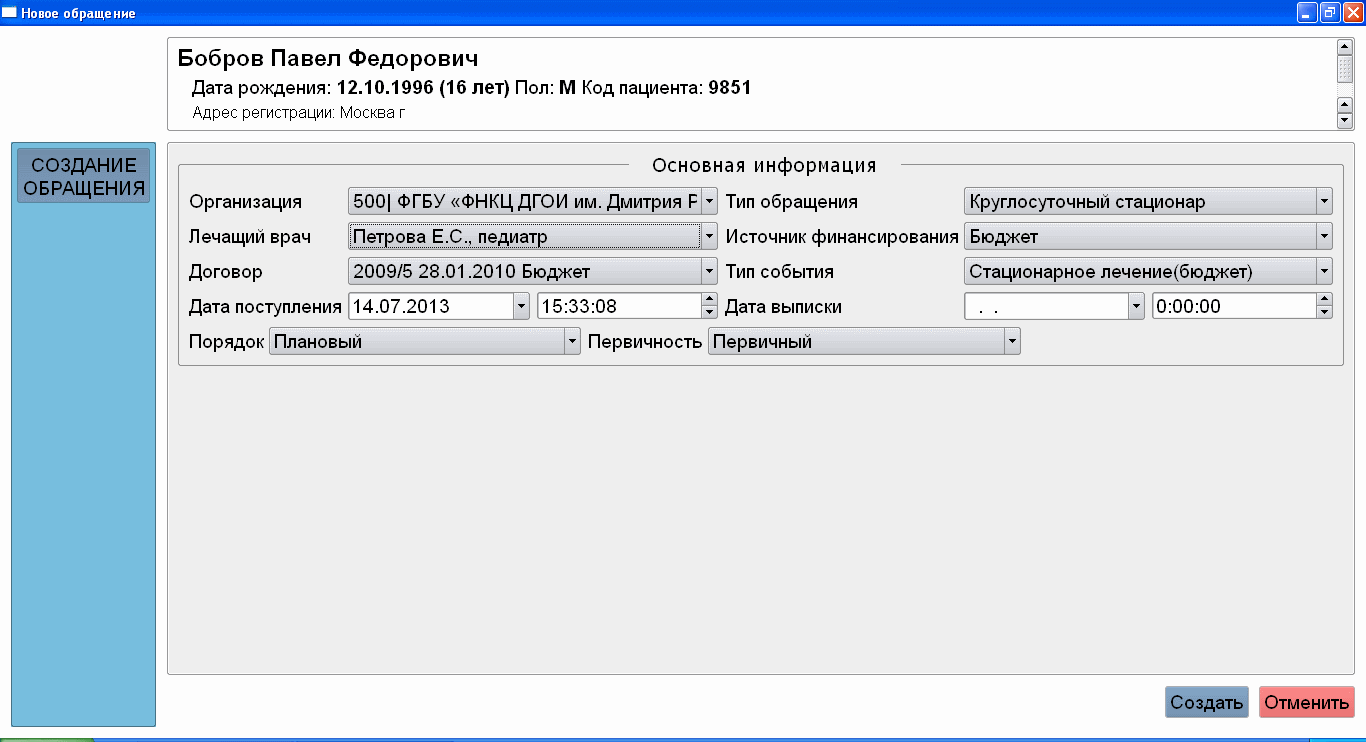
\includegraphics[width = 1\textwidth ,keepaspectratio]{st_obr_new}
   \caption{Окно регистрации нового обращения в стационар}
   \label{img_st_obr_new}
 \end{figure}

\begin{vnim}
 Поле \dm{Дата выписки} на данном этапе заполнять не нужно!
\end{vnim}
 
Окно \dm{Новое обращение} содержит следующие поля:
\begin{itemize}
 \item \dm{Организация} – наименование ЛПУ, в котором регистрируется случай обращения. По умолчанию указывается текущее ЛПУ.
 \item \dm{Тип обращения} выбирается из списка значение <<Стационар>> или <<Дневной стационар>>.
 \item \dm{Лечащий врач} – врач, который будет производить осмотр пациента в приемном отделении.
 \item \dm{Источник финансирования} – канал оплаты обращения, выбирается из списка.
 \item \dm{Договор} – номер договора об оплате выбирается из списка. Состав списка зависит от выбранного источника финансирования.
 \item \dm{Тип события} – выбирается из списка. Состав списка изменяется в зависимости от выбранного типа обращения и источника финансирования.
 \item \dm{Дата поступления} – дата начала госпитализации;  по умолчанию устанавливается текущая дата и время. При необходимости дату и время можно изменить.
 \item \dm{Дата выписки} – дата и время завершения обслуживания по данному обращению. Должна заполняться врачом при закрытии случая обращения.
 \item \dm{Порядок} – выбирается из списка <<Плановый>> или <<Экстренный>>.
 \item \dm{Первичность} – выбирается из списка.
\end{itemize}

В результате описанных действий будет зарегистрирована новая карточка обращения (Рисунок \ref{img_st_obr_oi}).

\begin{figure}[!t]\centering
   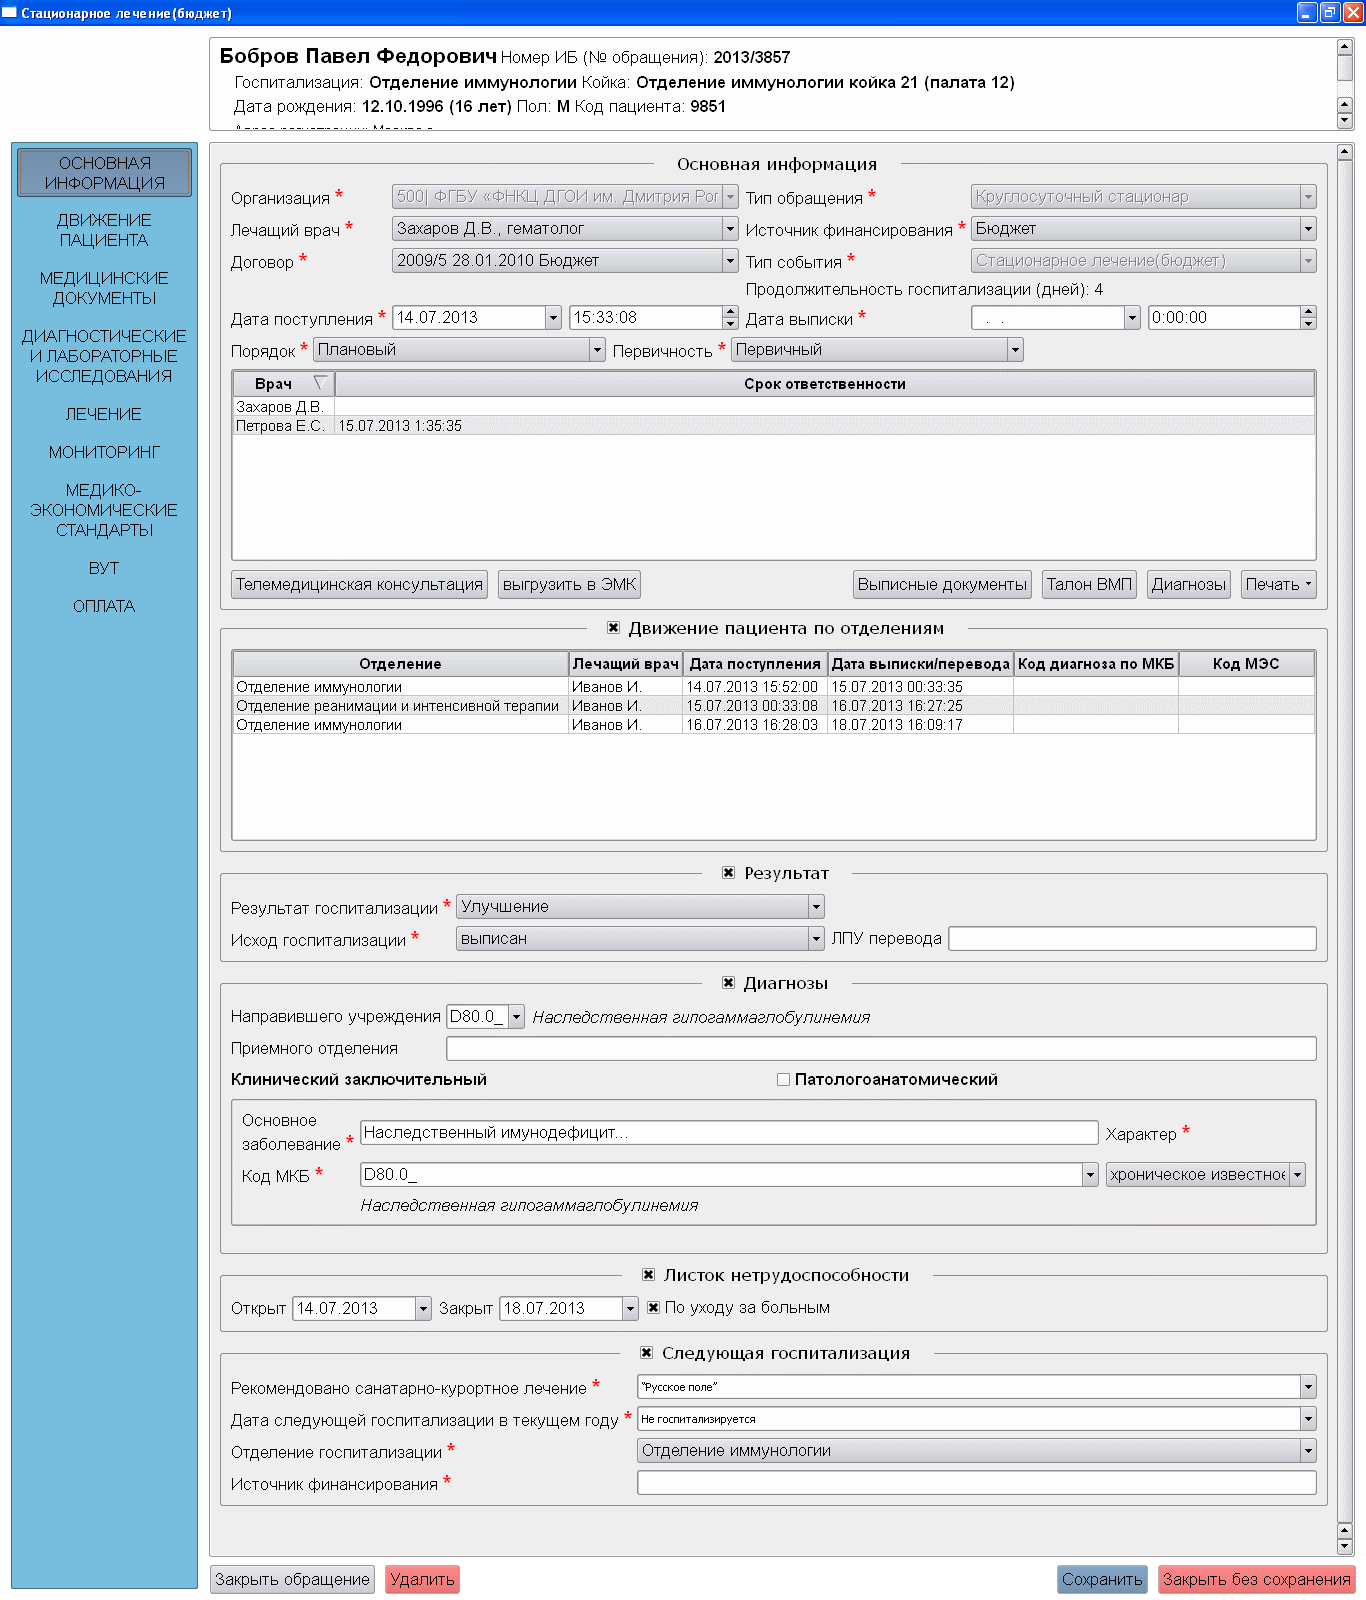
\includegraphics[width = 1\textwidth ,keepaspectratio]{st_obr_oi}
   \caption{Карточка обращения в стационар}
   \label{img_st_obr_oi}
 \end{figure}

\subsection{Карточка обращения в стационар} 

Карточка обращения в стационар (Рисунок \ref{img_st_obr_oi}) во многом совпадает с карточкой поликлинического обращения. На панели слева отображается список разделов карточки. Для перехода в соответствующий раздел, нужно щелкнуть левой кнопкой мыши по его названию на панели слева:
\begin{itemize}
 \item Раздел \dm{Основная информация} содержит общие сведения о случае обращения в стационар, которые учитываются в стат.талоне и других документах;
 \item Раздел \dm{Движение пациента} содержит информацию о поступлении пациента, его размещении на койке, переводах в другие отделения  и выписке;
 \item Раздел \dm{Медицинские документы} содержит результаты осмотров и консультаций врачей;
 \item Раздел \dm{Диагностические и лабораторные исследования} содержит направления на исследования и их результаты;
 \item Раздел \dm{Лечение} содержит лист медикаментозных назначений, направления на физиотерапевтическое и другие виды лечения и данные об их выполнении;
 \item Раздел \dm{Мониторинг} содержит информацию о группе крови и резус-факторе пациента. Информация представлена в виде таблицы, в которой ведется история внесения информации о группе крови и резус-факторе. Для каждой записи указывается фамилия врача, внесшего информацию, и дата установления;
 \item Раздел \dm{Медико-экономические стандарты} дает возможность проверки соответствия назначений врача медико-экономическим стандартам по данному заболеванию.
 \item Раздел \dm{Оплата} содержит данные об оплате (для платных услуг).
\end{itemize}
 
В зависимости от роли пользователя в системе, некоторые разделы могут быть недоступны ему.

\subsubsection{Раздел <<Основная информация>>}

Данный раздел разбит на несколько секций, каждая из которых содержит определенную группу данных. Отображением всех секций, кроме секции \dm{Основная информация}, можно управлять. Для отображения секции нужно установить флажок \putx~слева от названия секции, для ее скрытия -- снять этот флажок. Большая часть информации переносится в текущий раздел автоматически по результатам заполнения документов в других разделах.

Секция \dm{Основная информация} содержит данные, указанные при регистрации обращения. Некоторые из этих данных являются недоступными для редактирования, так как их изменение потребует изменения типа обращения, что невозможно. При изменении полей \dm{Источник финансирования} и \dm{Договор} появляется диалоговое окно (Рисунок \ref{img_st_obr_dlg}). Изменения вносятся в поле только после нажатия кнопки \btn{Да}.

\begin{figure}[ht]\centering
   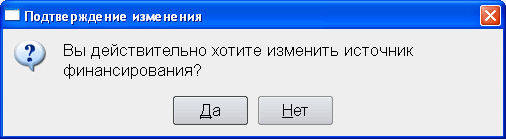
\includegraphics[width = 0.6\textwidth ,keepaspectratio]{st_obr_dlg}
   \caption{Запрос подтверждения изменения источника финансирования}
   \label{img_st_obr_dlg}
\end{figure}

\begin{prim}
 Если было создано обращение неверного типа или неверно выбрано название организации, следует удалить данное обращение, воспользовавшись кнопкой \btn{Удалить} в левом нижнем углу карточки обращения и создать новое обращение с правильными параметрами.
\end{prim} 

Значение поля \dm{Лечащий врач} необходимо изменять каждый раз при передаче пациента другому лечащему врачу. Как правило, лечащий врач изменяется при регистрации каждого нового действия в разделе \dm{Движения пациента}. Все изменения лечащего врача фиксируются в таблице ниже. Таблица доступна только для просмотра, т.е. редактирование ее невозможно.

Поле \dm{Дата поступления} так же не доступно для изменения. Поле \dm{Дата выписки} заполняется врачом в момент выписки пациента. Если поле \dm{Дата выписки} не заполнено, считается, что пациент находится на госпитализации, исходя из этого, вычисляется \dm{Продолжительность госпитализации}.

В таблице секции \dm{Движение пациента по отделениям} отображаются все перемещения пациента по отделениям, указанные в разделе \dm{Движение пациента} карточки обращения. Данные доступны только для просмотра. Для редактирования данных следует перейти в раздел \dm{Движение пациентов} карточки обращения.

В секции \dm{Результат} указывается результат госпитализации пациента. Поле \dm{Результат госпитализации} необходимо заполнить в данном разделе, выбрав соответствующее значение из списка, перед закрытием обращения. Значение поля \dm{Исход госпитализации} автоматически берется из действия <<Выписка>> раздела \dm{Движение пациента}. Изменения поля \dm{Исход госпитализации} в текущем разделе невозможно. Для внесения изменений, необходимо отредактировать выписку пациента.

Данные секции \dm{Диагнозы} заполняются автоматически на основании медицинских документов пациента. В частности, диагнозы поступления и приемного отделения отображаются из соответствующих полей действия <<Поступление>> раздела \dm{Движение пациента} карточки обращения; клинический диагноз берется из медицинского документа <<Обоснование клинического диагноза>>, а при его отсутствии – из последнего <<Первичного осмотра…>>; патологоанатомический – из патологоанатомического заключения (Протокола патологоанатомического исследования). В разделе \dm{Основная информация} диагнозы представлены только для просмотра, редактирование их в данном разделе невозможно. Для изменения диагноза следует отредактировать соответствующий медицинский документ.

В секции \dm{Листок нетрудоспособности} можно указать информацию о выданном пациенту или сопровождающему его лицу листе нетрудоспособности. Ввод информации осуществляется непосредственно в данной секции. Для сохранения информации следует нажать кнопку \btn{Сохранить} в низу окна.

Данные секции \dm{Следующая госпитализация} берутся из действия <<Выписка>> раздела \dm{Движение пациента} карточки обращения. В данном разделе они представлены для просмотра. Для изменения информации в данной секции следует отредактировать <<Выписку>> пациента.

В нижней части раздела \dm{Основная информация} расположен ряд кнопок. Нажатие кнопки \btn{выгрузить в ЭМК}  позволяет сохранить все медицинские документы пациента, зарегистрированные в рамках текущего обращения, в файл. При нажатии кнопки \btn{Выписные документы} открывается окно, содержащее список выписных документов пациента (Рисунок \ref{img_st_obr_docs}). Документы можно открыть для просмотра и редактирования. Способы работы с документами в данном окне аналогичен работе с документами в разделе \dm{Медицинские документы} карточки обращения (см. раздел \ref{st_obr_md})

\begin{figure}[ht]\centering
   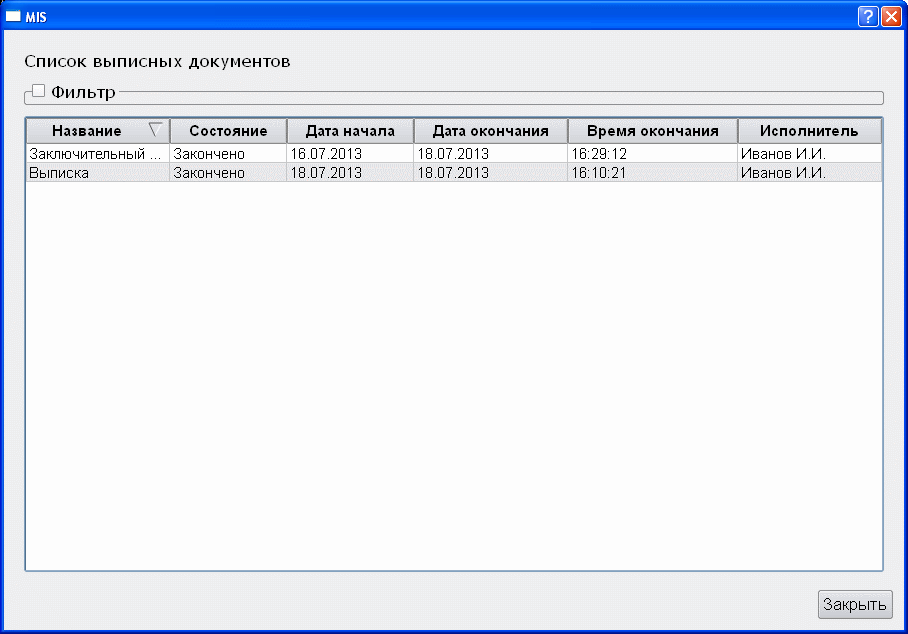
\includegraphics[width = 0.7\textwidth ,keepaspectratio]{st_obr_docs}
   \caption{Выписные документы пациента}
   \label{img_st_obr_docs}
\end{figure}
 
Кнопка \btn{Талон ВМП}  позволяет зарегистрировать талон ВМП для пациента. При нажатии на кнопку \btn{Диагнозы} открывается окно (Рисунок \ref{img_st_obr_dz}), содержащее список всех диагнозов, зарегистрированных в составе медицинских документов пациента.

\begin{figure}[ht!]\centering
   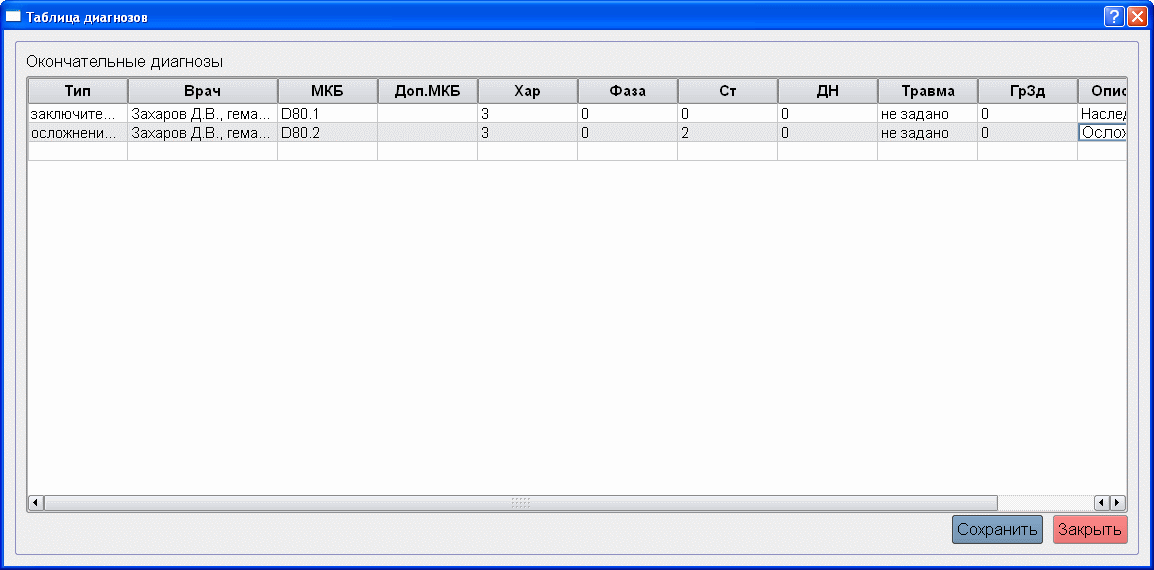
\includegraphics[width = 0.8\textwidth ,keepaspectratio]{st_obr_dz}
   \caption{Таблица диагнозов обращения}
   \label{img_st_obr_dz}
\end{figure}

Кнопка \btn{Печать} позволяет выполнить предварительный просмотр и вывести на печать различные медицинские документы пациента, относящиеся  к текущему случаю обращения в стационар. По этой кнопке возможен вывод на печать сразу нескольких медицинских документов пациента (например, всех направлений, всех результатов исследований или всех осмотров врача, назначенных или выполненных в рамках текущего обращения). Для печати документа следует нажать кнопку \btn{Печать} в центральной части окна, в появившемся меню выбрать нужную печатную форма и щелкнуть по ее названию левой кнопкой мыши. Откроется окно предварительного просмотра печатной формы (Рисунок \ref{img_st_obr_prn1}). Для отправки документа на принтер, необходимо нажать кнопку \btn{Печатать}, для сохранения документа в файл – кнопку \btn{Сохранить}, затем в открывшемся окне выбрать папку для сохранения файла, ввести название и нажать кнопку \btn{Сохранить}.

\begin{figure}[ht]\centering
   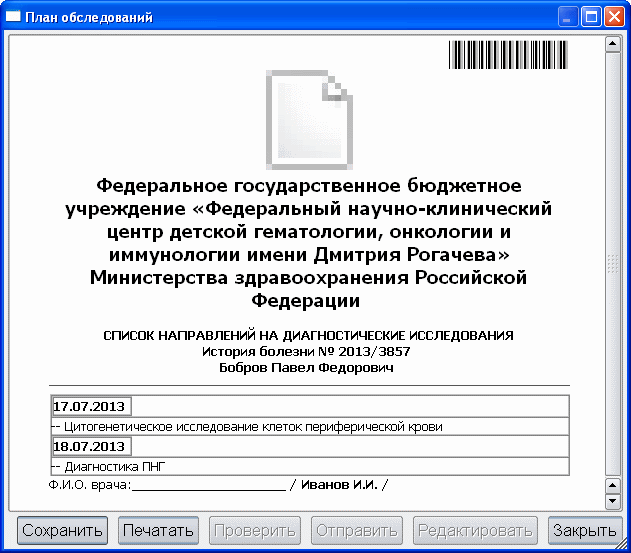
\includegraphics[width = 0.7\textwidth ,keepaspectratio]{st_obr_prn1}
   \caption{Предварительный просмотр печати}
   \label{img_st_obr_prn1}
\end{figure}
 
\subsubsection{Работа с карточкой обращения}

В нижней части окна карточки обращения имеются следующие кнопки:
\begin{itemize}
 \item При нажатии на кнопку \btn{Закрыть обращение} выполняется закрытие обращения (см. раздел \ref{st_obr_close})
 \item \btn{Удалить} Нажатие на данную кнопку приводит к появлению диалогового окна, содержащего запрос: <<Вы уверены, что хотите удалить это обращение?>>. \textbf{Будьте внимательны! При выборе варианта <<Да, удалить>> происходит удаление всего обращения.}
 \item \btn{Сохранить} При нажатии на кнопку происходит сохранение данных обращения. Если операция сохранения прошла успешно, появляется сообщение <<Данные успешно сохранены>>.
 \item \btn{Закрыть без сохранения} Данная кнопка аналогична кнопке \btn{Отмена} в некоторых других карточках. При нажатии на нее карточка обращения закрывается, а все несохраненные ранее изменения теряются.
\end{itemize}

\subsubsection{Редактирование карточки обращения}

Для редактирования обращения необходимо найти пациента (используя фильтры), к которому относится обращение в картотеке пациентов на вкладке \dm{Пациенты} и щелкнть по нему левой кнопкой мыши. После чего нужно перейти на вкладку \dm{Обращение} картотеки пациентов, найти там требуемое обращение и дважды щелкнуть по нему левой кнопкой мыши либо выделить найденное обращение и нажать кнопку \keys{F4} на клавиатуре или кнопку \btn{Редактировать(F4)} в нижней части окна. В результате любого из описанных действий карточка обращения откроется для просмотра и редактирования данных.

Можно выполнить поиск обращения пациента непосредственно на вкладке \dm{Обращение} (в обход вкладки \dm{Пациенты}), используя поиск для всех пациентов картотеки, и открыть его на редактирование клавишей \keys{F4} на клавиатуре либо кнопкой \btn{Редактировать(F4)}. 

Открытие обращения на редактирование возможно так же через стационарный монитор (см. раздел \ref{st_mon})

\subsection{Регистрация движения пациента}

Регистрация мест размещения пациента производится в карточке стационарного обращения в разделе \dm{Движение пациента}.

В центральной части окна раздела расположены кнопки для добавления действий и флажок \dm{Фильтр}. При установке флажка открывается дополнительная область, где можно задать критерии фильтрации действий указанного раздела. Работа с фильтром аналогична описанной в разделе \ref{pol_obr_mdfiltr}

Для редактирования какого-либо из ранее созданных действий можно дважды щелкнуть по нужному действию левой кнопкой мыши или щелкнуть по нему правой кнопкой мыши и в появившемся контекстном меню выбрать пункт \dm{Открыть действие}.

\begin{prim}
Если нужно открыть карточку действия для просмотра, то можно щелкнуть по нему правой кнопкой мыши и в появившемся контекстном меню выбрать пункт \dm{Открыть действие только для чтения}. Редактирование открытого таким образом действия будет невозможно, что позволит избежать случайных изменений. Открытие действий только на чтение позволяет просматривать его сразу нескольким пользователям и не препятствует редактированию другими пользователями.
\end{prim}

Для удаления ошибочно созданного действия нужно щелкнуть по нему правой кнопкой мыши и в открывшемся меню выбрать пункт \dm{Удалить действие}. На экране появится диалоговое окно, запрашивающее подтверждение удаления. При подтверждении операции выбранное действие будет удалено.

В верхней части окна редактирования (создания) любого из действий раздела \dm{Движение пациента} присутствуют следующие поля:
\begin{itemize}
 \item \dm{Назначено} – дата и время назначения действия. Для действия <<Поступление>> по умолчанию устанавливается дата и время регистрации обращения. Для остальных действий движения – по умолчанию устанавливается текущая дата и время.
 \item Флажок \dm{Срочно} нужно установить для экстренных действий.
 \item \dm{План} – плановая дата завершения действия.
 \item \dm{Назначил} – фамилия назначившего сотрудника. Для действий движения по умолчанию указывается фамилия сотрудника, создавшего данное действие.
 \item \dm{Состояние} – для действий движения используется 2 состояния: <<Начато>> и <<Закончено>>. Краткосрочные действия, такие как <<Поступление>> или <<Выписка>> по умолчанию создаются в статусе <<Закончено>>. Действия, имеющие продолжительный характер, такие как пребывание в отделении (действий <<Движение>>) создаются в состоянии <<Начато>> и должны оставаться в этом статусе до выписки или перевода пациента из отделения.
 \item \dm{Начато} – дата и время начала выполнения действия. По умолчанию ставится текущие дата и время.
 \item \dm{Выполнено} – время завершения действия. Заполняется автоматически при изменении значения в поле \dm{Состояние} на <<Закончено>>. 
 \item \dm{Исполнитель} – фамилия сотрудника, зарегистрировавшего действие. Как правило, для действий движения значение данного поля совпадает с полем \dm{Назначил}.
 \item \dm{Кабинет} – не заполняется для действий движения.
 \item \dm{Количество} – всегда должно быть равно 1.
 \item \dm{УЕТ} – не заполняется для действий движения.
 \item \dm{Примечания} – в поле можно ввести с клавиатуры дополнительные сведения, если они есть. Поле не является обязательным для заполнения.
\end{itemize}
 
Все перечисленные поля доступны для редактирования.

Состав полей определяется настройками системы и может незначительно отличаться в различных ЛПУ.

Для некоторых действий движения предусмотрена возможность печати соответствующих документов. Для направления документа на печать следует выполнить одно из описанных ниже действий:
\begin{itemize}
 \item Щелкнуть правой кнопкой мыши по названию действия и в появившемся контекстном меню выбрать пункт \dm{Печать}.
 \item Открыть карточку действия для редактирования или только для чтения и нажать кнопку \btn{Печать} в правом нижнем углу открывшегося окна.
\end{itemize}

\begin{figure}[ht!]\centering
   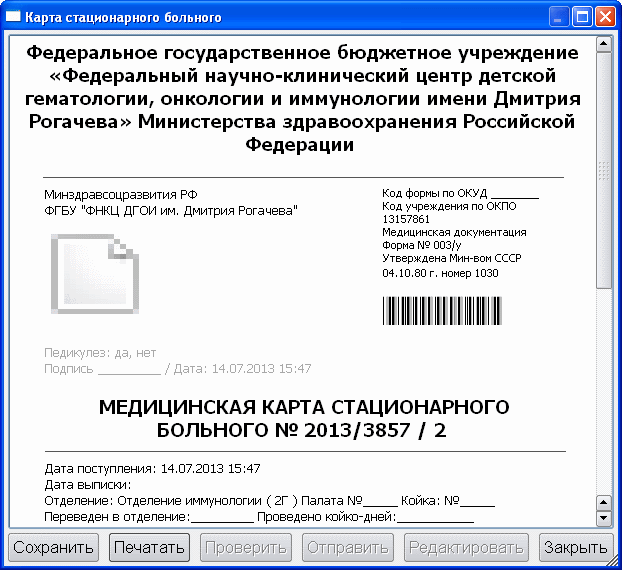
\includegraphics[width = 0.6\textwidth ,keepaspectratio]{st_obr_prn2}
   \caption{Окно предварительного просмотра печатной формы}
   \label{img_st_obr_prn2}
\end{figure}
 
Если для выбранного действия предусмотрено несколько печатных форм, то после выполнения одной из описанных операций появится дополнительное меню, где необходимо выбрать название нужной печатной формы, щелкнув по нему левой кнопкой мыши, после чего откроется окно предварительного просмотра печатной формы (Рисунок \ref{img_st_obr_prn2}). Если для выбранного действия предусмотрена единственная печатная форма, то окно предварительного просмотра откроется сразу же после выполнения одной из описанных операций. Если для действия не предусмотрено печатных форм, то пункт меню \dm{Печать} и кнопка \btn{Печать} будут недоступны.

Для направления документа на принтер, следует нажать кнопку \btn{Печатать} в окне предварительного просмотра печатной формы.

\subsubsection{Регистрация поступления пациента}

При поступлении пациента в приемное отделение стационара, до направления его в клиническое отделение, необходимо в разделе \dm{Движение пациента} зарегистрировать действие <<Поступление>>. Как правило, регистрацию данного действия выполняет медсестра – регистратор приемного отделения.

\begin{figure}[ht]\centering
   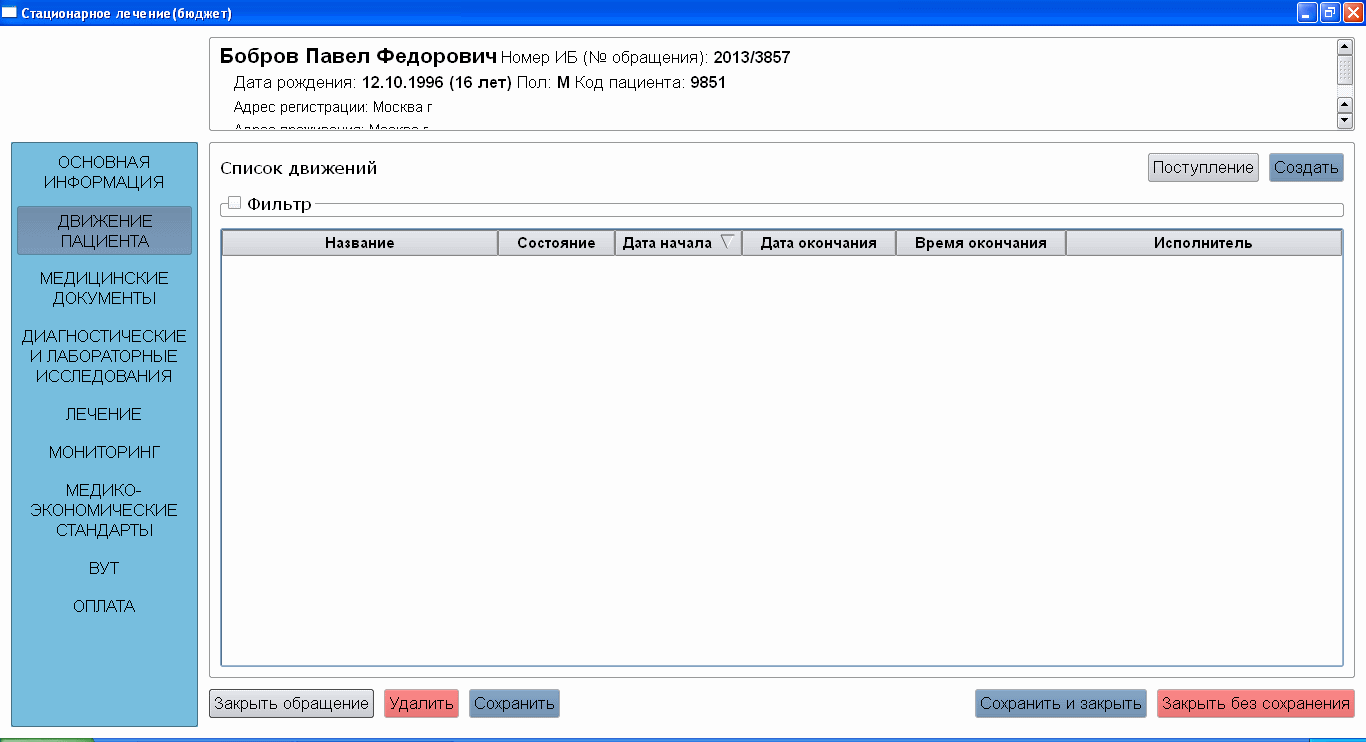
\includegraphics[width = 1\textwidth ,keepaspectratio]{st_obr_dv}
   \caption{Карточка обращения в стационар. Раздел <<Движение пациента>>}
   \label{img_st_obr_dv}
\end{figure}

\begin{figure}[ht]\centering
   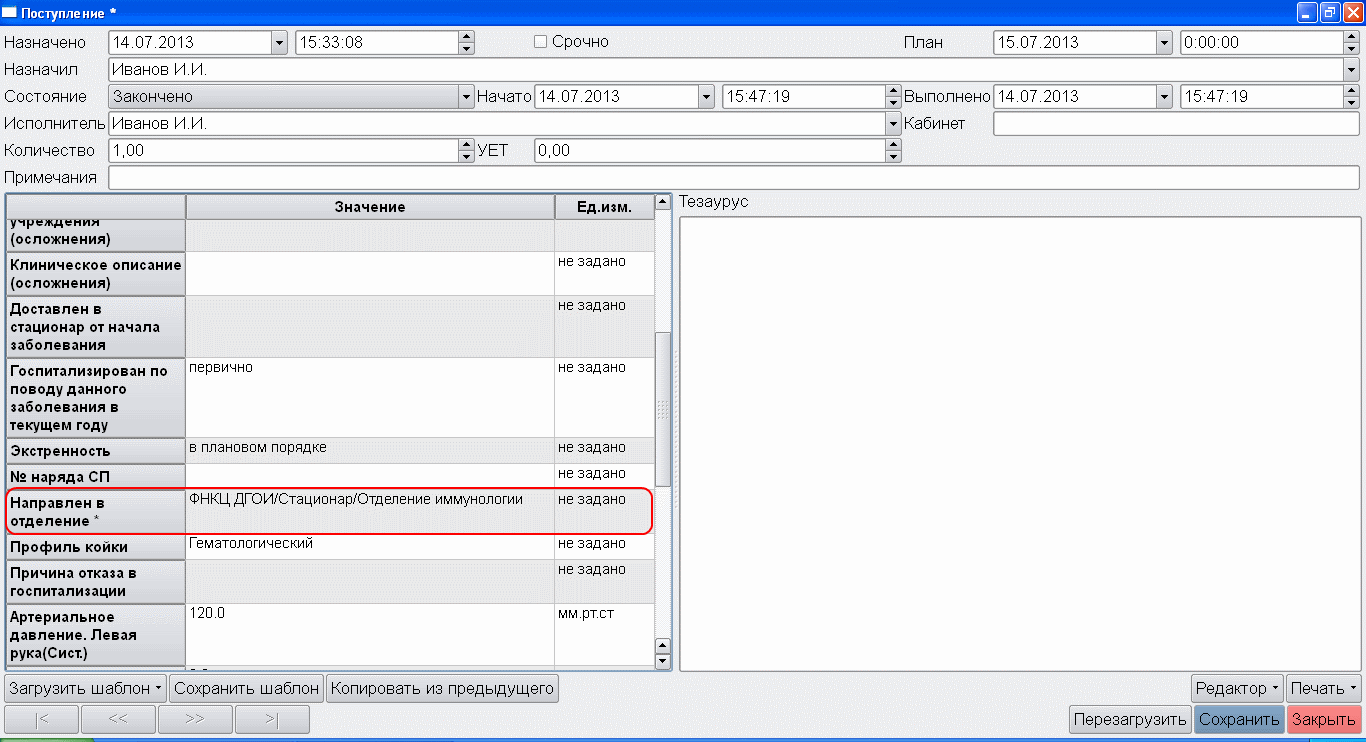
\includegraphics[width = 1\textwidth ,keepaspectratio]{st_obr_dvcard}
   \caption{Окно регистрации поступления в стационар}
   \label{img_st_obr_dvcard}
\end{figure}
  
Для регистрации поступления пациента требуется:
\begin{enumerate}
 \item Найти текущее обращение в стационар пациента любым способом и открыть карточку обращения на редактирование (если она еще не открыта).
 \item Перейти в раздел \dm{Движение пациента} (Рисунок \ref{img_st_obr_dz}).
 \item Нажать кнопку \btn{Поступление} или кнопку \btn{Создать} в средней части окна.
 \item В случае нажатия кнопки \btn{Создать} , необходимо из открывшегося списка действий двойным щелчком левой кнопки мыши выбрать <<Поступление>> и нажать кнопку \btn{OK} в правом нижнем углу окна, в результате будет открыто окно регистрации действия поступления. В случае нажатия кнопки  \btn{Поступление} сразу будет открыто окно регистрации выбранного действия (Рисунок \ref{img_st_obr_dvcard}).
 \item В окне регистрации поступления следует ввести все необходимые данные. Состав и назначение полей верхней части окна описаны выше. В основной части окна состав и последовательность полей определяется локальными настройками системы и может отличаться в различных ЛПУ. Ряд полей нужно заполнять вручную, в других следует выбирать значение из списка. Для активации поля ввода или списка выбора нужно щелкнуть по соответствующей ячейке в колонке \dm{Значение} левой кнопкой мыши. При любых настройках системы в действии <<Поступление>> необходимо заполнить поля \dm{Отделение поступления} и \dm{Направлен в отделение}. В качестве отделения поступления, как правило, указывается <<Приемное отделение>>, но это значение можно изменить при необходимости.
 \item После того как все необходимые поля заполнены, нужно нажать кнопку \btn{Сохранить}. Окно регистрации поступления закроется, а в списке действий раздела \dm{Движение пациентов} появится новая запись.
\end{enumerate}

\begin{vnim}
 В составе обращения может быть создано только одно действие <<Поступление>>. При попытке создать второе такое действие выдается соответствующее предупреждение.
\end{vnim}
 
Как правило, из карточки действия <<Поступление>> можно распечатать обложку истории болезни пациента (Ф. 003/У) и статистическую карту выбывшего из стационара (Ф. 066/У). Возможность печати действий движения описана выше. Печать этих документов доступна так же из раздела \dm{Общая информация} карточки обращения.

\subsubsection{Регистрация поступления в отделение} \label{st_obr_dvdv}

При поступлении пациента в клиническое отделение и размещении его на койке постовая медсестра должна зафиксировать данное событие в ФТМИС. Для этого следует зарегистрировать действие <<Движение>> в разделе \dm{Движение пациента} карточки обращения.

\begin{vnim}
 Регистрация действия <<Движение>> возможна только при наличии действия <<Поступление>> и отсутствии других действий <<Движение>>, находящихся в состоянии <<Начато>>. Если <<Поступление>> не создано, необходимо сообщить об этом в приемное отделение. Если при переводе пациента из другого отделения остается незакрытым действие <<Движение>>, необходимо сообщить об этом в отделение, откуда переводится пациент.
\end{vnim}
 
Для регистрации <<Движения>> следует выполнить следующие действия:
\begin{enumerate}
 \item Открыть карточку текущего обращения пациента и перейти в ней в раздел \dm{Движение пациента}.
 \item Нажать кнопку \btn{Движение} или \btn{Создать} в средней части окна.
 \item При нажатии кнопки \btn{Движение} сразу открывается окно редактирования действия (Рисунок \ref{img_st_obr_dvdv}). При нажатии кнопки \btn{Создать} требуется в открывшемся окне двойным щелчком левой кнопки мыши выбрать <<Движение>> и нажать кнопку \btn{OK} в правом нижнем углу окна, после чего так же откроется окно редактирования действия (Рисунок \ref{img_st_obr_dvdv}).
 \item Заполнить поля в шапке и табличной части действия.
 \item Нажать кнопку \btn{Сохранить}, в результате чего окно редактирования действия закроется, а в списке действий раздела \dm{Движение пациентов} появится новая запись.
\end{enumerate}

\begin{figure}[ht]\centering
   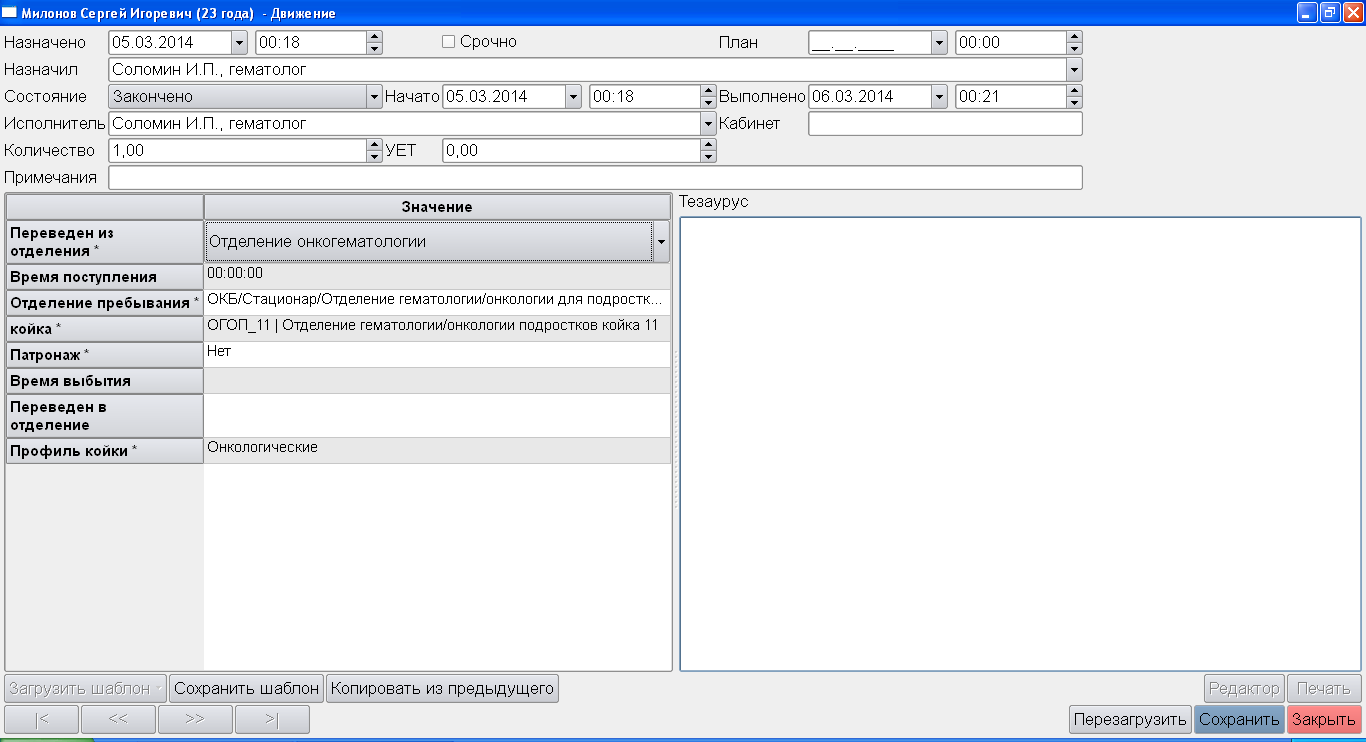
\includegraphics[width = 1\textwidth ,keepaspectratio]{st_obr_dvdv}
   \caption{Окно регистрации поступления в отделение}
   \label{img_st_obr_dvdv}
 \end{figure}
 
При заполнении окна регистрации шапка аналогична описанной в предыдущем разделе. При создании действия <<Движение>> ему автоматически присваивается состояние <<Начато>>, которое должно сохраняться на протяжении всего времени пребывания пациента в отделении. Состав полей в табличной части определяется настройками системы и может отличаться в каждом ЛПУ. При любых настройках действие <<Поступление>> должно содержать поля \dm{Переведен из отделения}, \dm{Отделение пребывания}, \dm{Койка}, \dm{Профиль койки} и \dm{Патронаж}. При правильном оформлении действия <<Поступление>>, поля \dm{Переведен из отделения} и \dm{Отделение пребывания} будет заполнено автоматически. Значение поля \dm{Патронаж} выбирается из списка. В поле \dm{Койка} следует выбрать номер койки, на которой будет размещен пациент. Согласно выбранной койке будет автоматически заполнено поле \dm{Профиль койки}. При выборе койки для размещения пациента, по умолчанию раскрывается список коек отделения пребывания, соответствующих полу пациента. Серым цветом окрашены занятые койки, черным – свободные (Рисунок \ref{img_st_obr_vibkoik}).

\begin{figure}[ht]\centering
   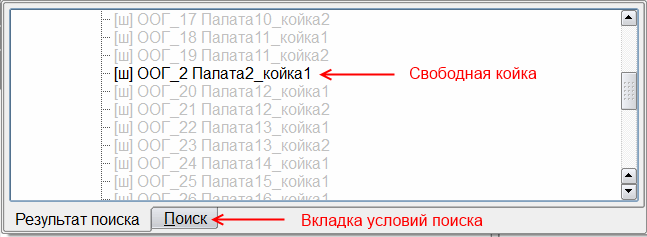
\includegraphics[width = 0.8\textwidth ,keepaspectratio]{st_obr_vibkoik}
   \caption{Список коек}
   \label{img_st_obr_vibkoik}
\end{figure}

Для изменения критериев поиска коек следует перейти на вкладку \dm{Поиск} (Рисунок \ref{img_st_obr_findkoik}). На этой вкладке можно задать следующие параметры поиска:
\begin{itemize}
 \item \dm{Подразделение} – отделение, в котором располагается койка.
 \item \dm{Пол} – для подбора палаты в соответствии с полом пациента.
 \item \dm{Возраст} – для подбора палаты в соответствии с возрастом пациента. Как правило различают взрослые, детские палаты, палаты для новорожденных.
 \item \dm{Профиль койки} выбирается из списка.
 \item \dm{Тип койки} выбирается из списка.
 \item \dm{Штат} – можно выбрать только штатные (<<Да>>) или заштатные (<<Нет>>) койки.
\end{itemize}
 
Все заполненные параметры поиска связаны между собой по <<И>>, т.е. в результат поиска попадают только те койки, для которых выполняются все указанные условия.

\begin{figure}[ht]\centering
   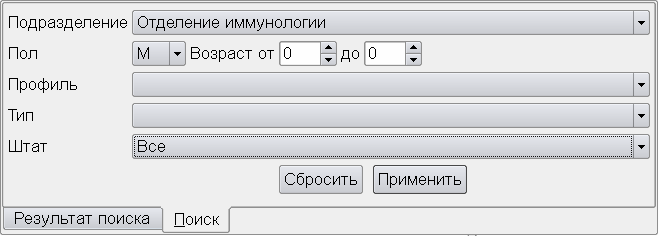
\includegraphics[width = 0.8\textwidth ,keepaspectratio]{st_obr_findkoik}
   \caption{Поиск коек}
   \label{img_st_obr_findkoik}
\end{figure}
 
После заполнения всех критериев поиска следует нажать кнопку \btn{Применить}. Будет осуществлен автоматический переход на вкладку \dm{Результаты поиска} (Рисунок \ref{img_st_obr_vibkoik}), где отобразится список коек в соответствии с новыми параметрами поиска.

Для возврата к первоначальным настройкам поиска (по умолчанию) можно нажать кнопку \btn{Сбросить} , а затем кнопку \btn{Применить} . На вкладке \dm{Результаты поиска} отобразится список коек отделения, в которое направлен пациент, соответствующих его полу.

\begin{vnim}
 При регистрации действия <<Движение>> часть полей в табличной части окна (такие как \dm{Переведен в отделение}, \dm{Время выбытия}) следует оставить пустыми. Они заполняются при выписке или переводе пациента в другое отделение.
\end{vnim}

\begin{vnim}
 В составе обращения может быть только одно действие <<Движение>> в состоянии <<Начато>>. Для регистрации нового действия данного типа, нужно закрыть предыдущее действие, указав направление выбытия пациента.
\end{vnim}

\subsubsection{Регистрация перевода пациента в другое отделение}

Регистрация перевода в другое отделение состоит из 2-х этапов:

\textbf{1 этап}. Закрытие действия <<Движение>> в отделении выбытия пациента. Для этого следует открыть карточку действия, находящегося в статусе <<Начато>> для редактирования и выполнить следующие шаги:
\begin{enumerate}
 \item В верхней части окна изменить состояние действия на <<Закончено>>.
 \item Проконтролировать (и при необходимости изменить) дату и время перевода в поле \dm{Выполнено} в верхней части окна.
 \item В табличной части окна, в поле \dm{Переведен в отделение}, выбрать из дерева структуры ЛПУ название отделения, в которое направляется пациент, заполнить поле \dm{Время выбытия} (Рисунок \ref{img_st_obr_dvvib}).
 \item Сохранить изменения, нажав кнопку \btn{Сохранить} в правом нижнем углу окна.
\end{enumerate}

\begin{figure}[ht]\centering
   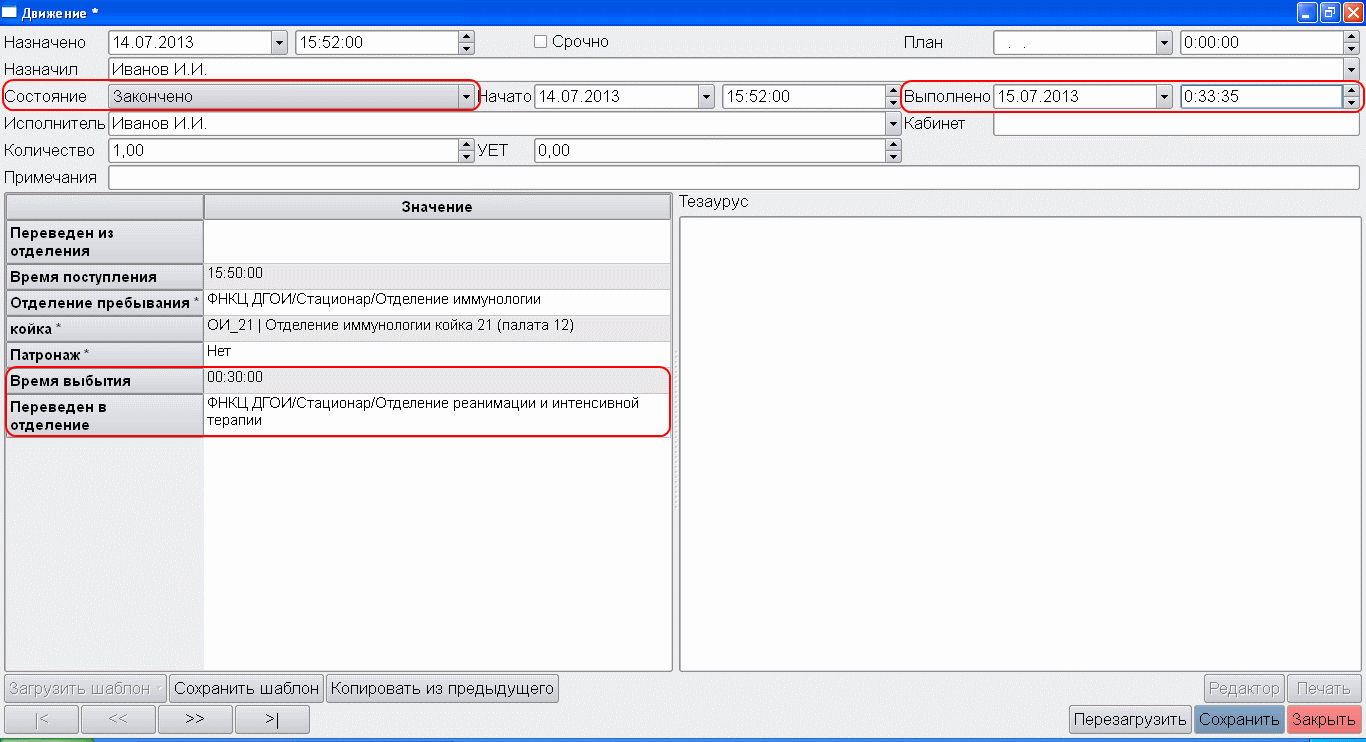
\includegraphics[width = 1\textwidth ,keepaspectratio]{st_obr_dvvib}
   \caption{Регистрация выбытия пациента из отделения}
   \label{img_st_obr_dvvib}
 \end{figure}
 
\textbf{2 этап}. Регистрация поступления пациента в принимающем отделении. Для этого необходимо зарегистрировать новое действие <<Движение>>. При правильном оформлении выбытия пациента из предыдущего отделения, поля \dm{Переведен из отделения} и \dm{Отделение пребывания} во вновь созданном действии <<Движение>> будут заполнены автоматически соответствующими значениями (Рисунок \ref{img_st_obr_dvvib2}). Порядок регистрации пациента в отделении подробно рассмотрен в разделе \ref{st_obr_dvdv}

\begin{figure}[ht]\centering
   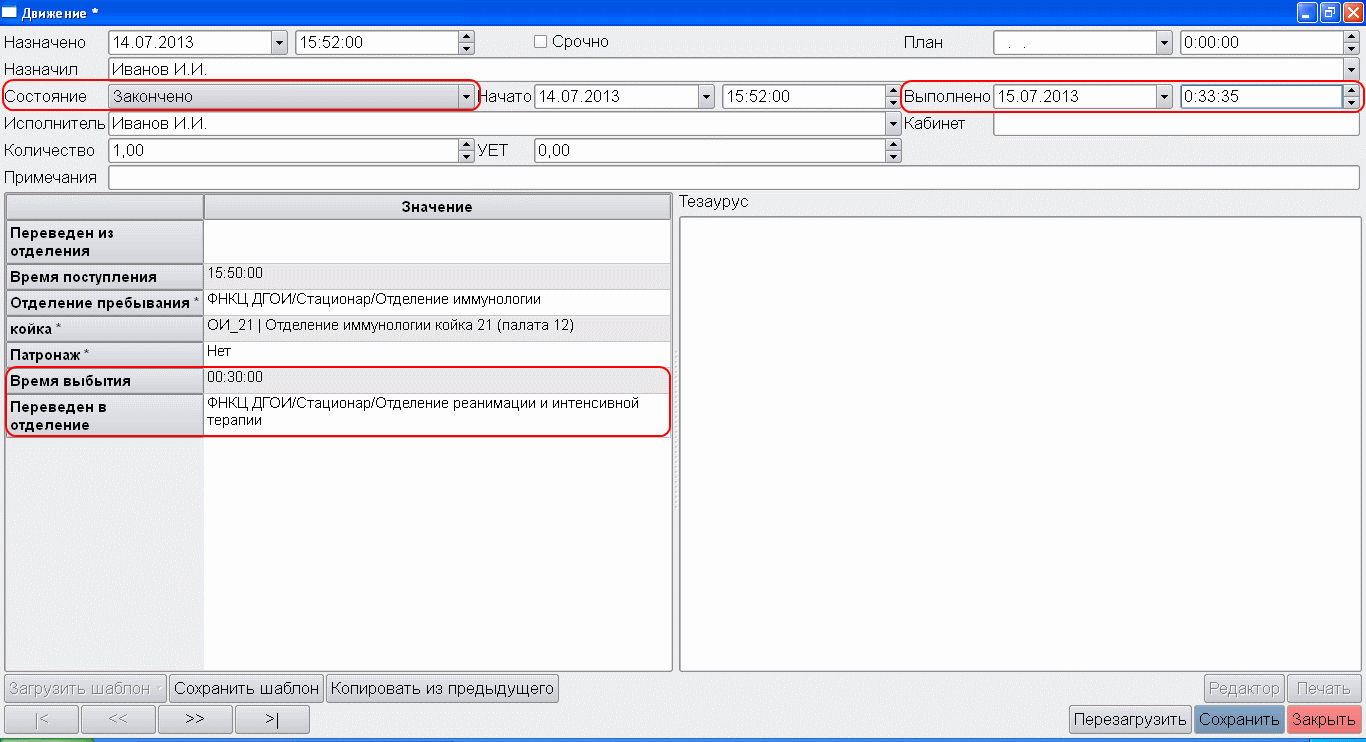
\includegraphics[width = 1\textwidth ,keepaspectratio]{st_obr_dvvib2}
   \caption{Регистрация движения пациента в принимающем отделении}
   \label{img_st_obr_dvvib2}
\end{figure}

\subsubsection{Регистрация выписки пациента}

\begin{figure}[ht]\centering
   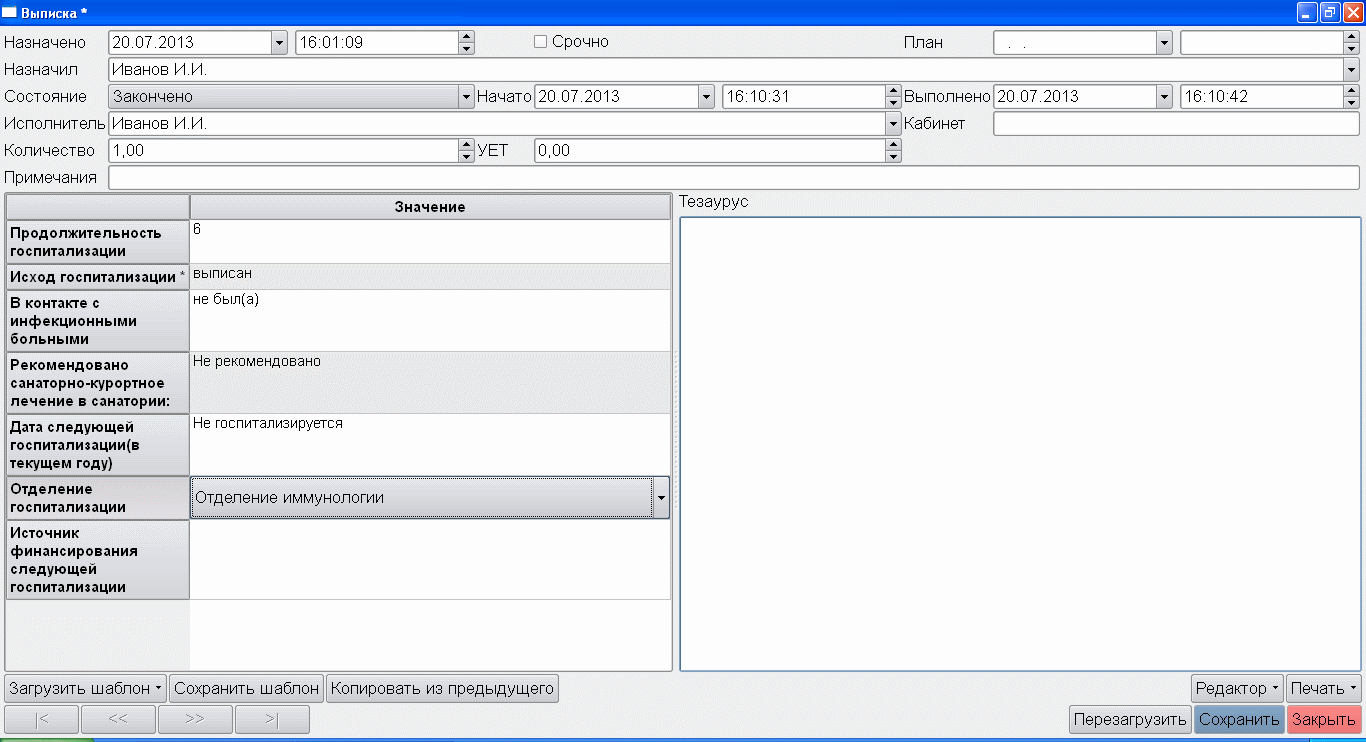
\includegraphics[width = 1\textwidth ,keepaspectratio]{st_obr_dvvip}
   \caption{Регистрация выписки пациента}
   \label{img_st_obr_dvvip}
\end{figure}

Для регистрации выписки пациента из ЛПУ необходимо выполнить следующие шаги:
\begin{enumerate}
 \item Закрыть последнее действие <<Движение>>. Для этого следует изменить состояние действия на <<Закончено>>, в поле \dm{Выполнено} в верхней части окна указать дату и время выписки пациента, в ячейке \dm{Время выбытия} табличной части окна указать время выписки пациента и сохранить сделанные изменения.
 \item В разделе \dm{Движение пациента} зарегистрировать новое действие <<Выписка>>. Для этого следует нажать кнопку \btn{Выписка} в средней части окна или нажать кнопку \btn{Создать} , а затем в списке действий двойным щелчком левой кнопки мыши выбрать <<Выписка>> и нажать кнопку \btn{OK}  в правом нижнем углу окна. Откроется окно редактирования действия <<Выписка>> для пациента (Рисунок \ref{img_st_obr_dvvip}).
 \item В верхней части окна в поле \dm{Состояние} установить значение <<Закончено>>, в поле \dm{Выполнено} указать дату и время выписки пациента.
 \item При правильном оформлении предыдущих действий раздела \dm{Движение пациентов}, поля \dm{Продолжительность госпитализации} и \dm{Отделение госпитализации} табличной части окна будут заполнены автоматически соответствующими значениями. Состав полей табличной части окна определяется настройками системы и может отличаться в различных ЛПУ. Необходимо заполнить  поля табличной части окна соответствующими значениями. Вне зависимости от настроек, требуется обязательно заполнить поле \dm{Исход госпитализации}, выбрав соответствующее значение из списка (Рисунок \ref{img_st_obr_dvvip}).
 \item Сохранить действие, нажав кнопку \btn{Сохранить} в правом нижнем углу окна.
\end{enumerate}

\begin{vnim}
 В составе обращения может быть создано только одно действие <<Выписка>>. При попытке создать второе такое действие выдается соответствующее предупреждение.
\end{vnim}

\subsubsection{Постановка пациента в очередь на госпитализацию}

В \tmis предусмотрена возможность планирования госпитализаций. Для постановки пациента в очередь на госпитализацию, необходимо зарегистрировать пациента в системе, а затем зарегистрировать обращение в стационар для него. В качестве даты поступления при этом нужно указать дату включения пациента в план госпитализаций.

После этого в разделе \dm{Движение пациента} следует зарегистрировать новое действие <<Планирование>>. Для этого необходимо:
\begin{enumerate}
 \item Нажать кнопку \btn{Создать} в средней части окна, а затем в списке действий двойным щелчком левой кнопки мыши выбрать <<Планирование>> и нажать кнопку \btn{OK}  в правом нижнем углу окна. Откроется окно редактирования действия <<Планирование>> для пациента (Рисунок \ref{img_st_obr_dvplan}).
 \item В верхней части окна в поле \dm{План} указать плановую дату госпитализации пациента.
 \item Заполнить табличную часть окна. Обязательно нужно указать планируемое отделение госпитализации и желательно планируемую койку для размещения пациента.
 \item Сохранить действие, нажав кнопку \btn{Сохранить}  в правом нижнем углу окна.
\end{enumerate}

\begin{figure}[ht]\centering
   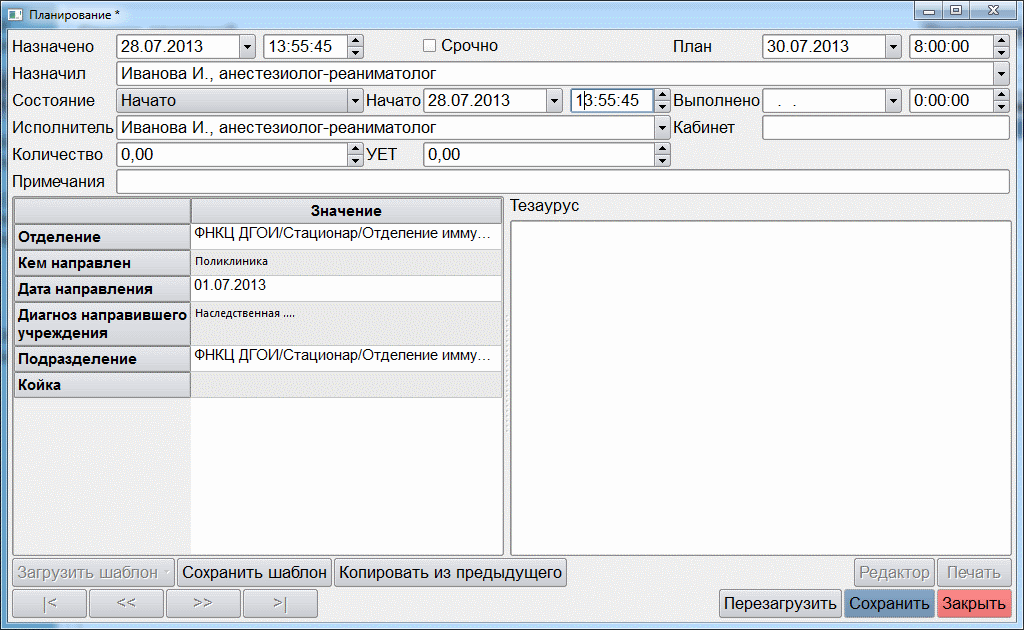
\includegraphics[width = 1\textwidth ,keepaspectratio]{st_obr_dvplan}
   \caption{Планирование госпитализации пациента}
   \label{img_st_obr_dvplan}
\end{figure} 

\subsection{Оформление медицинских документов пациента} \label{st_obr_md}

\subsubsection{Регистрация первичного осмотра}

Регистрация первичного осмотра пациента производится в разделе \dm{Медицинские документы} карточки обращения. Допускается наличие нескольких первичных осмотров в составе одного обращения (например, первичный осмотр в приемном отделении, первичный осмотр в отделении пребывания, первичный осмотр в новом отделении после перевода). Порядок регистрации осмотров подробно рассмотрен в разделе \ref{pol_obr_md}

\begin{prim}
 Использование шаблонов документов при заполнении результатов первичного осмотра может значительно сократить время, затрачиваемое на оформление документа (см. раздел \ref{pol_pattern})
\end{prim}

\subsubsection{Регистрация осмотра дежурного врача}
 
В разделе \dm{Медицинские документы}, в средней части окна, предусмотрена кнопка быстрой регистрации осмотра дежурного врача \btn{Дежурный врач}. При нажатии на эту кнопку сразу открывается окно редактирования результатов осмотра дежурного врача (Рисунок \ref{img_st_obr_mdd}). Это окно так же можно вызвать, если нажать кнопку \btn{Создать}  в средней части окна, затем двойным щелчком левой кнопки мыши выбрать <<Дежурный врач осмотр>> или<<Осмотр дежурного врача>> из списка и подтвердить выбор нажатием кнопки \btn{OK} в правом нижнем углу окна. 

\begin{figure}[ht]\centering
   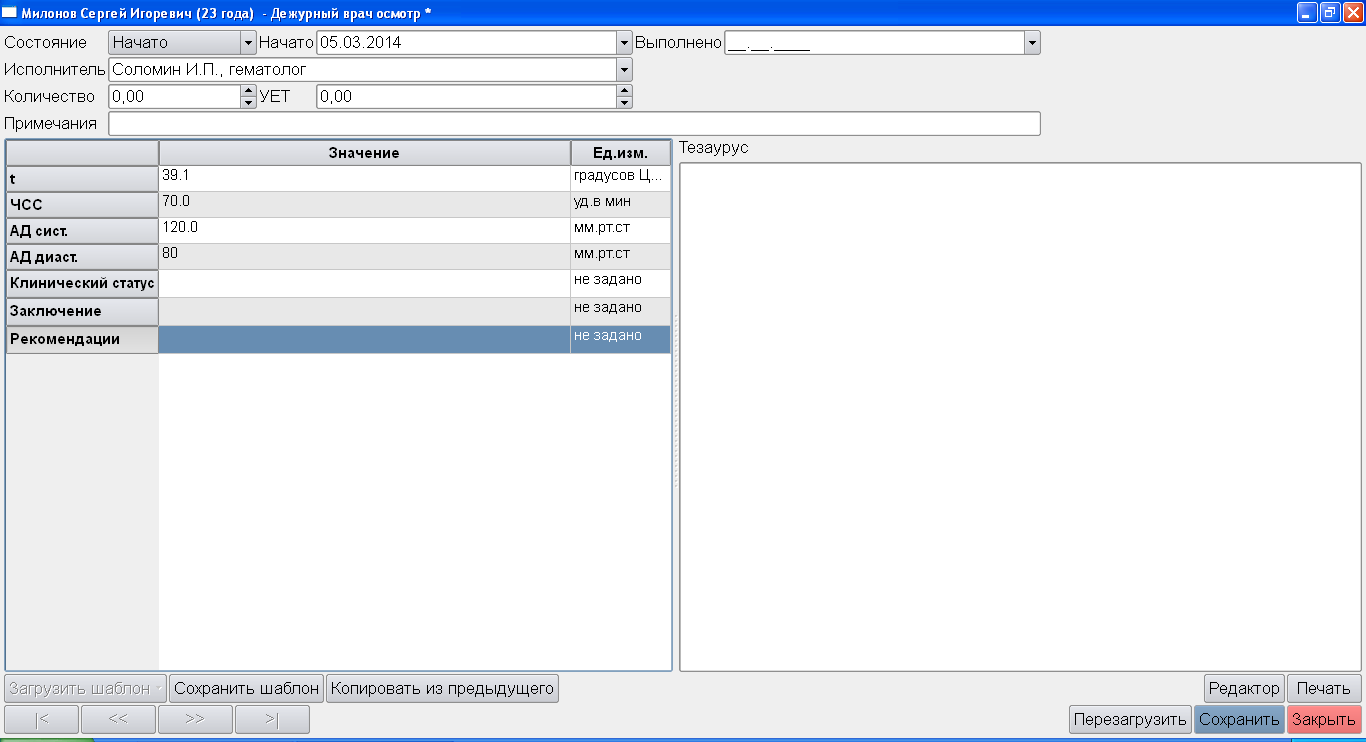
\includegraphics[width = 1\textwidth ,keepaspectratio]{st_obr_mdd}
   \caption{Регистрация осмотра дежурного врача}
   \label{img_st_obr_mdd}
\end{figure} 

Необходимо заполнить результаты осмотра в табличной части окна (Рисунок \ref{img_st_obr_mdd}), в верхней части окна изменить состояние действия на <<Завершено>>, проконтролировать (при необходимости, изменить), чтобы в полях \dm{Начато} и \dm{Выполнено} была указана дата выполнения осмотра, в поле \dm{Исполнитель} – фамилия врача, выполнившего осмотр, и нажать кнопку \btn{Сохранить}.

Порядок регистрации осмотра дежурного врача аналогичен порядку регистрации других осмотров и подробно рассмотрен в разделе \ref{pol_obr_md}

\subsubsection{Формирование эпикризов, обоснования клинического диагноза}

Регистрация переводных и выписных эпикризов, обоснований клинического диагноза и других медицинских документов, подводящих итог лечения пациента на определенном этапе, так же производится в разделе \dm{Медицинские документы} карточки обращения. Формирование документа аналогично формированию других медицинских документов и подробно рассмотрено в разделе \ref{pol_obr_md}

Отличительной особенностью данного типа документов является необходимость включения в него результатов исследований, проведенных во время диагностики и лечения пациента. В \tmis~существует возможность автоматического добавления в медицинский документ результатов исследований, проведенных в рамках текущего случая обращения пациента. Для этого следует установить курсор в поле \dm{Проведенные исследования (обследования)} табличной части окна редактирования медицинского документа, щелкнуть правой кнопкой мыши в любом месте активного поля редактирования и в появившемся контекстном меню выбрать пункт \dm{Заполнить}. Откроется окно выбора исследований, результаты которых можно автоматически занести в эпикриз (Рисунок \ref{img_st_obr_mdepik}).

\begin{figure}[ht]\centering
   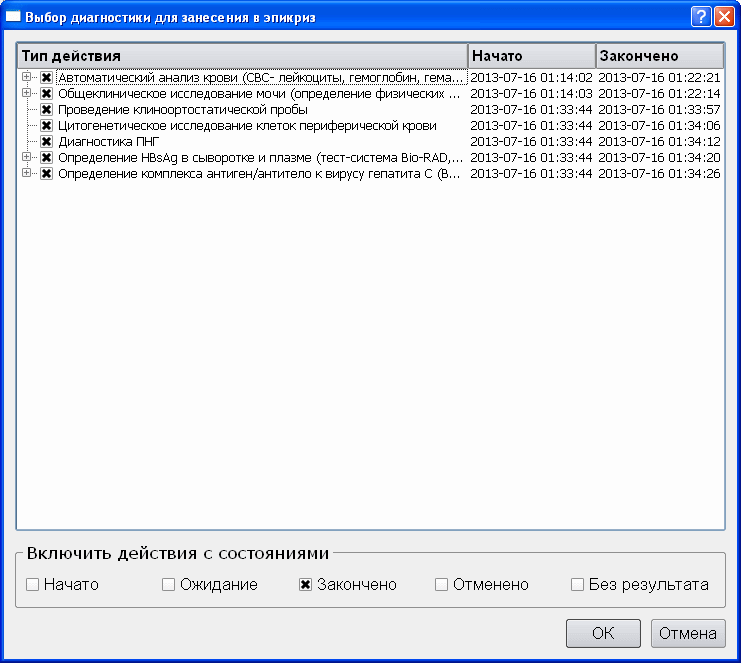
\includegraphics[width = 0.8\textwidth ,keepaspectratio]{st_obr_mdepik}
   \caption{Окно выбора исследований для занесения в эпикриз}
   \label{img_st_obr_mdepik}
\end{figure} 

В верхней части окна находится список наименований исследований, доступных для добавления в эпикриз. Установленный флажок рядом с названием исследования говорит о том, что результаты исследования будут включены в эпикриз. По умолчанию, флажки установлены для всех доступных исследований. Необходимо оставить флажки только напротив тех исследований, которые требуется включить в эпикриз, щелкнув по ним левой кнопкой мыши. Для исследований, состоящих из нескольких параметров, можно так же управлять набором параметров, которые войдут в эпикриз. Для этого нужно щелкнуть кнопку <<$+$>>, слева от названия исследования, и в раскрывшемся списке параметров снять флажки с тех, которые не должны войти в эпикриз. После того как все необходимые исследования отмечены, нужно нажать кнопку \btn{OK}  в правом нижнем углу окна, в результате чего в поле \dm{Проведенные исследования (обследования)} окна редактирования эпикриза будут добавлены результаты выбранных на предыдущем шаге исследований (Рисунок \ref{img_st_obr_mdepik2}). Данные доступны для редактирования и форматирования.

\begin{figure}[ht]\centering
   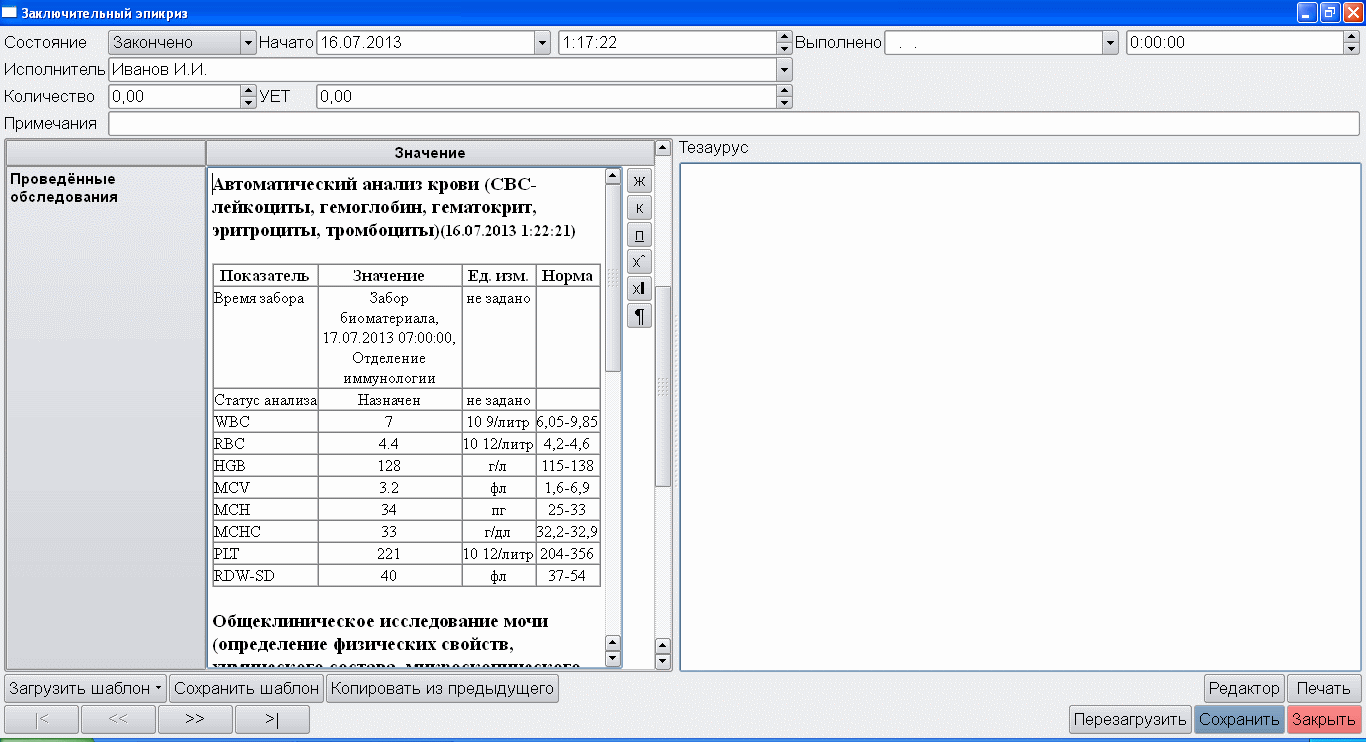
\includegraphics[width = 1\textwidth ,keepaspectratio]{st_obr_mdepik2}
   \caption{Автоматическое добавление результатов исследований в эпикриз}
   \label{img_st_obr_mdepik2}
\end{figure} 

По умолчанию в список исследований, доступных для добавления в эпикриз включаются только исследования, находящиеся в состоянии <<Закончено>>. Для того, чтобы включить в эпикриз исследования в любом другом состоянии, следует в нижней части окна выбора исследований (Рисунок \ref{img_st_obr_mdepik}) установить флажок рядом с соответствующим состоянием, после чего все исследования в выбранном состоянии появятся в списке, в верхней части окна.

Остальные поля медицинских документов данного типа нужно заполнять по общим принципам. После завершения работы с документом его следует сохранить, нажав кнопку \btn{Сохранить}  в правом нижнем углу окна.

\subsubsection{Регистрация направлений на исследования}

Регистрация направлений на исследования подробно рассмотрена в разделе \ref{pol_obr_is}

\subsubsection{Назначение лечения пациенту}

Регистрация направлений на физиотерапевтическое и другие виды лечения подробно описана в разделе \ref{pol_obr_lek}

\subsubsection{Лист назначений}

\paragraph{Формирование листа назначений}

Лист назначений возможно сформировать только для обращений стационарного типа. Доступ к листу назначений в карточке обращения имеют только врачи стационара.

Оформление листов назначений выполняется в разделе \dm{Лечение} карточки стационарного обращения. Для открытия листа назначений необходимо нажать кнопку \btn{Лист назначений}, в результате чего откроется новое окно \dm{Лист назначений} (Рисунок \ref{img_st_obr_ln}). В левой верхней части данного окна размещается информация о пациенте, для которого открыт лист назначений. В правом верхнем углу расположены параметры отображения листа назначения и легенда для назначений. В основной части окна размещается список назначений, в нижней части – примечание по листу назначений и управляющие кнопки.

\begin{figure}[ht]\centering
   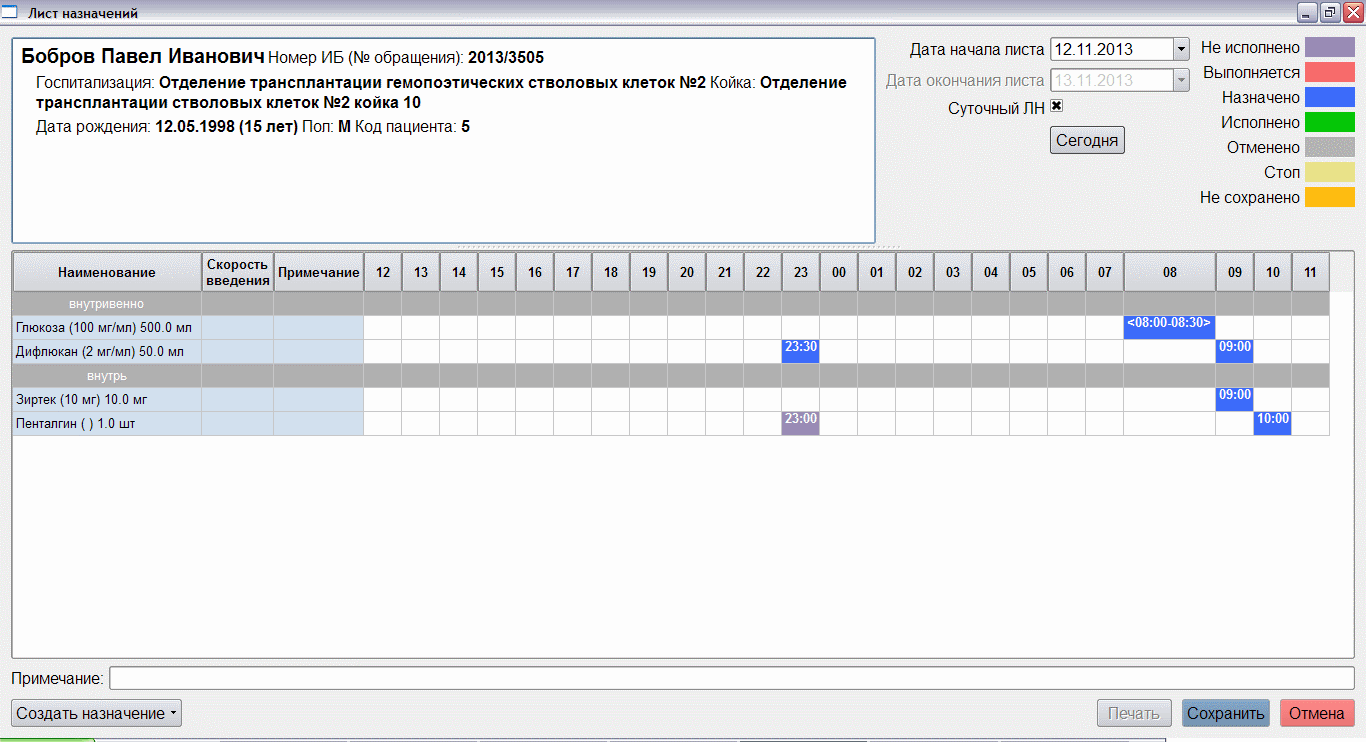
\includegraphics[width = 1\textwidth ,keepaspectratio]{st_obr_ln}
   \caption{Лист назначений. Основное окно}
   \label{img_st_obr_ln}
\end{figure} 

Лист назначений может отображаться в двух видах:
\begin{itemize}
 \item Суточный;
 \item За выбранный период.
\end{itemize}
 
Суточный лист назначений показывает назначения на текущие сутки, начиная со времени начала суток, принятого в ЛПУ (определяется настройками системы). Каждая ячейка листа соответствует одному часу. Для использования суточного листа назначений необходимо установить флажок \dm{Суточный} в правом верхнем углу окна. Можно просмотреть суточный лист назначений за любые сутки, выбрав соответствующую дату в поле \dm{Дата начала листа} в правом верхнем углу окна. Кнопка \btn{Сегодня} устанавливает в указанное поле текущую дату, что позволяет быстро вернуться к просмотру листа назначений на текущие сутки.

Лист назначений за выбранный период показывает назначения за период в несколько дней. Каждая ячейка листа при этом соответствует одним суткам. Для использования данного представления листа назначений необходимо в правом верхнем углу снять флажок \dm{Суточный} и указать даты начала и окончания периода отображения листа назначений в полях \dm{Дата начала листа} и \dm{Дата окончания листа} соответственно.

Для каждого лекарственного препарата создается отдельное назначение. Исключение составляют случаи, когда назначается смесь из нескольких препаратов, тогда все препараты смеси включаются в одно назначение. Если изменяется способ введения или доза препарата так же требуется создание нового назначения.

Для добавления нового назначения следует нажать кнопку \btn{Создать назначение} в левом нижнем углу окна и в появившемся списке выбрать тип медикаментозного назначения: терапия, анальгезия, химиотерапия, инфузионная терапия. Откроется новое окно \dm{Назначение} (Рисунок \ref{img_st_obr_lnnazn}).

\begin{figure}[ht]\centering
   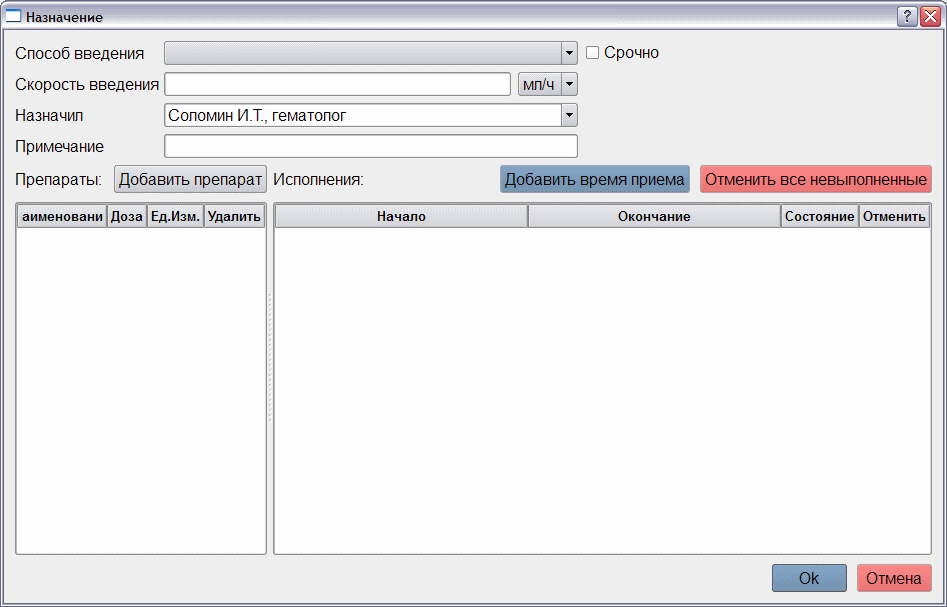
\includegraphics[width = 0.8\textwidth ,keepaspectratio]{st_obr_lnnazn}
   \caption{Новое назначение}
   \label{img_st_obr_lnnazn}
\end{figure} 

В данном окне необходимо указать данные нового медикаментозного назначения:
\begin{itemize}
 \item В поле \dm{Способ введения} нужно выбрать из списка способ введения назначаемого лекарственного препарата;
 \item Флажок \dm{Срочно} необходимо поставить, если назначение сделано в экстренном порядке;
 \item В поле \dm{Скорость введения препарата} значение вводится с клавиатуры;
 \item Единица измерения скорости введения выбирается из справочника справа от поля \dm{Скорость введения препарата};
 \item В поле \dm{Назначил} указывается фамилия текущего пользователя (от имени которого осуществлен вход в систему). Изменение значения данного поля невозможно;
 \item В поле \dm{Примечание} можно указать дополнительную информацию по данному назначению.
\end{itemize}
 
После того как поля в верхней части заполнены, необходимо добавить назначаемый препарат либо список препаратов в назначение. Для этого следует нажать кнопку \btn{Добавить препарат}. В поле \dm{Наименование} в левом нижнем углу формы раскроется окно для поиска нужного препарата (Рисунок \ref{img_st_obr_lnnazn2}). Необходимо ввести название препарата или действующего вещества в верхнее поле раскрывшегося окна. По мере ввода названия (начиная с третьего символа), система будет выводить список подходящих по начальным буквам наименования или действующего вещества препаратов. Для исключения ошибок при вводе наименования препарата рекомендуется выбрать его из предлагаемого списка двойным щелчком левой кнопки мыши. Допускается так же ввести наименование препарата полностью и нажать клавишу \keys{Enter} на клавиатуре. После того как требуемый препарат выбран или введен, в нижней части окна поиска появится список найденных препаратов.

\begin{figure}[ht]\centering
   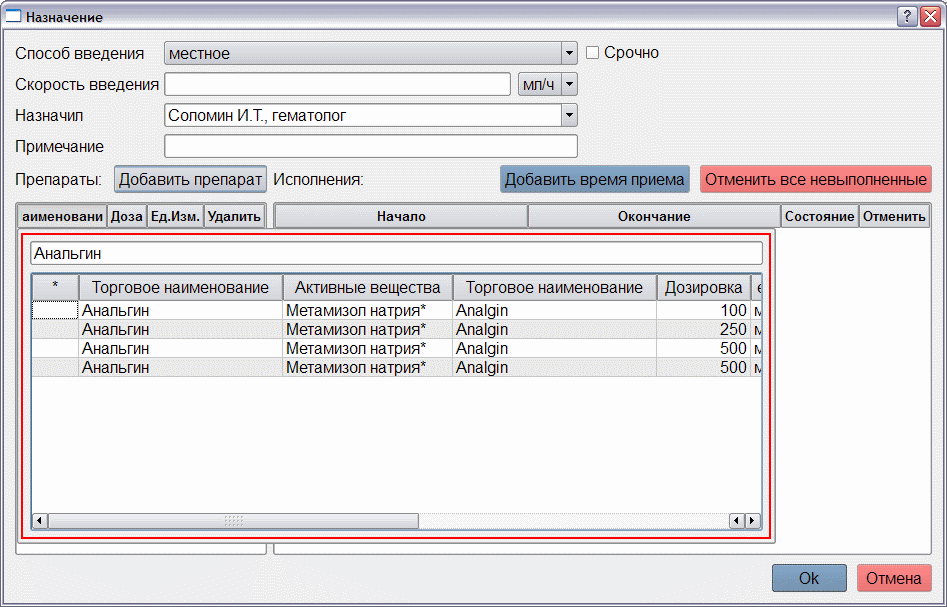
\includegraphics[width = 0.8\textwidth ,keepaspectratio]{st_obr_lnnazn2}
   \caption{Добавление препарата в назначение}
   \label{img_st_obr_lnnazn2}
\end{figure} 

В зависимости от наличия препарата в ЛПУ, строка с его наименованием будет окрашена в определенный цвет:
\begin{itemize}
 \item 	Синий – препарат имеется на складе отделения;
 \item Зеленый – препарат имеется на складе ЛПУ;
 \item Желтый – препарат имеется на складе другого отделения ЛПУ;
 \item Красный – препарат отсутствует в ЛПУ.
\end{itemize}
 
\begin{prim}
 При отсутствии интеграции с системой <<1С: Аптека>> строки будут иметь белый или серый цвет.
\end{prim}

Препараты, срок годности которых подходит к концу (составляет менее 30 \% допустимого срока хранения), помечаются символом <<*>>.

Следует выбрать нужный препарат в соответствующей форме выпуска из предложенного списка двойным щелчком левой кнопки мыши, в ячейке \dm{Доза} указать дозу разового приема в указанных в поле \dm{Ед.изм.} единицах измерения. Единица измерения подбирается автоматически при выборе препарата в зависимости от выбранной формы выпуска медикамента. В некоторых случаях могут предлагаться на выбор несколько единиц измерения, например <<мг>> и <<шт>> для таблеток.

Для добавления еще одного препарата в назначение, необходимо снова нажать кнопку \btn{Добавить препарат}  и повторить описанные выше действия. Система не устанавливает ограничений по количеству препаратов, которые могут содержаться в одном назначении.

Если необходимо удалить какой-либо из только что добавленных в назначение препаратов, следует нажать кнопку 
\includegraphics{x_big} , справа от его наименования, а затем подтвердить удаление в появившемся диалоговом окне <<Вы действительно хотите удалить препарат?>>.

\begin{vnim}
 Удаление препаратов из назначения возможно только для новых назначений, пока не выполнено их сохранение в базе данных. Если требуется изменить состав препаратов в сохраненном назначении, необходимо отменить это назначение  полностью и создать новое назначение с обновленным составом препаратов
\end{vnim}
 
После того как список препаратов в назначении сформирован, необходимо добавить время его приема. Для этого следует нажать кнопку \btn{Добавить время приема} . В таблице ниже появится новая строка, куда следует ввести данные о назначенном времени приема. Таблица содержит следующие поля:
\begin{itemize}
 \item \dm{Начало} – дата и время выполнения либо начала выполнения назначения. Поле обязательно для заполнения.
 \item \dm{Окончание} – дата и время окончания выполнения назначения. Заполняется только для назначений, имеющих длительный характер выполнения. 
 \item \dm{Состояние} – текущее состояние назначения. Может принимать значения <<Назначено>>, <<Выполнено>>, <<Отменено>>.
 \item \dm{Отменить} – в данном столбце располагаются кнопки   для отмены выполнения назначений. Отменить назначение может только лечащий или дежурный врач.
\end{itemize}
 
Для указания времени выполнения процедур, имеющих продолжительный характер (например, инфузии), необходимо заполнить поля \dm{Начало} и \dm{Окончание}, указав в них дату и время начала и окончания процедуры соответственно. Назначение должно выполняться непрерывно в течение всего указанного интервала.

Если необходимо задать время выполнения кратковременной процедуры (например, прием таблетки), то следует указать только дату и время начала.

Для назначения может быть добавлено несколько времен (периодов) приема. Если первый из периодов приема для назначения имел продолжительный характер (т.е. для периода были заданы время начала и окончания выполнения), то все остальные периоды так же должны иметь продолжительный характер. 

Каждое назначение должно обязательно содержать хотя бы один препарат и хотя бы одно время приема. Для каждого препарата в составе назначения в обязательном порядке должна быть указана доза.

После того, как карточка нового назначения заполнена, нужно нажать кнопку \btn{OK} , после чего будет осуществлен возврат к листу назначений, где появится новая запись о назначении. Наименование назначения будет окрашено в оранжевый цвет, сигнализируя о том, что назначение не сохранено. Время выполнения нового назначения будет окрашено полосами желтого цвета и цвета, соответствующего состоянию созданного назначения (в соответствии с легендой, расположенной в правом верхнем углу окна). Например, если назначение создано заранее (до начала его выполнения), то время его выполнения будет окрашено в сине-желтые полосы.

\begin{vnim}
 Нажатие на кнопку \btn{OK} в карточке назначения (Рисунок \ref{img_st_obr_lnnazn}) не сохраняет изменения в базе данных. Сохранение назначений выполняется из окна листа назначений кнопкой \btn{Сохранить}.
\end{vnim}
 
Описанным способом можно добавить необходимое количество назначений, используя кнопку \btn{Создать назначение}.

Все назначения в листе назначений группируются по способу введения.

\begin{prim}
 После того как лист назначений сформирован полностью, но еще не сохранен, рекомендуется еще раз проверить правильность всех вновь добавленных назначений, так как после сохранения назначений, их редактирование будет ограничено. Открытие назначения на редактирования осуществляется двойным щелчком мыши по соответствующей строке в листе назначений.
\end{prim}
 
После того как назначения добавлены в лист назначений, необходимо выполнить их сохранение. Для этого нужно нажать кнопку \btn{Сохранить}  в правом нижнем углу окна. При этом все наименования назначений, ранее окрашенные в оранжевый цвет, будут окрашены в голубой. Время исполнения новых назначений так же будет окрашено в цвет, соответствующий его состоянию.

\paragraph{Редактирование листа назначений}

После сохранения назначений в листе назначения, на их налагаются следующие ограничения:
\begin{itemize}
 \item Удаление назначений из листа назначений невозможно.
 \item Невозможно добавление, удаление, редактирование назначенных препаратов и дозы в назначении. Если необходимо изменить состав препаратов или дозы в назначении, следует отменить данное назначение кнопкой \btn{Отменить все неисполненные}  в карточке назначения и создать новое с учетом всех необходимых изменений.
 \item Невозможно изменить или удалить время выполнения назначения. При необходимости изменения времени выполнения, нужно это время выполнения отменить и добавить новое время выполнения с учетом изменений.
\end{itemize}
 
Для редактирования листа назначений необходимо:
\begin{enumerate}
 \item Нажать кнопку \btn{Лист назначений}  в разделе \dm{Лечение} карточки стационарного обращения.
 \item Дважды щелкнуть левой кнопкой мыши по наименованию назначения в листе назначений. Откроется карточка выбранного назначения.
 \item Внести необходимые изменения в карточку назначения и нажать кнопку \btn{OK}.
 \item Выполнить редактирование других назначений в листе (если необходимо).
 \item Нажать кнопку \btn{Сохранить}.
\end{enumerate}
 
При редактировании ранее сохраненных назначений возможно изменение следующих полей: \dm{Способ введения}, \dm{Скорость введения}, флажок \dm{Срочно}, \dm{Примечание}. Так же возможна отмена назначенного времени выполнения и добавление новых интервалов времени выполнения.

\paragraph{Управление выполнением назначений}

Для каждого времени приема может быть задано одно из следующих состояний:
\begin{itemize}
 \item \dm{Назначено} – назначение создано, но время приема еще не наступило.
 \item \dm{Выполняется} – назначение создано, и время приема совпадает с текущим временем. В данное сосотояние назначения переводятся автоматически, как правило, за 15 минут до времени начала приема и выходит из него так же автоматически после времени окончания приема, если в течение этого времени не выполнено изменение состояния вручную. Интервал времени, добавляемый к времени выполнения определяется настройками системы.
 \item \dm{Исполнено} – установлена отметка об исполнении данного назначения. Отметка может быть установлена только после наступления времени приема.
 \item \dm{Не исполнено} – время выполнения назначения прошло, но отметка об исполнении назначения не установлена.
 \item \dm{Отменено} – назначение было создано, а затем отменено на каком-либо из этапов выполнения. Можно отменить любое назначение, кроме исполненного.
\end{itemize}

Отметку об исполнении можно проставить только для времени приема, которое уже наступило или прошло. С другой стороны, редактирование состояния времени приема, которое уже прошло, возможно выполнять только в течение периода времени, заданного в настройках системы (как правило, 24 часа). После истечения этого времени, изменение состояния времени приема становится недоступно.

После смены состояния одного или нескольких интервалов необходимо сохранить изменения, нажав кнопку \btn{Сохранить} листа назначений.

На рисунке \ref{img_st_obr_lnsch} представлены варианты перехода назначений между статусами. В результате, любое назначение остается в одном из 3-х состояний: <<Исполнено>>, <<Не исполнено>> или <<Отменено>>.

\begin{figure}[ht]\centering
   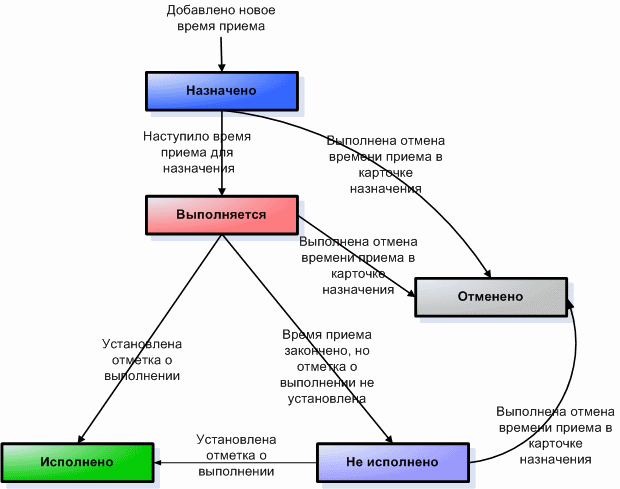
\includegraphics[width = 1\textwidth ,keepaspectratio]{st_obr_lnsch}
   \caption{Варианты перехода состояний выполнения назначений}
   \label{img_st_obr_lnsch}
\end{figure} 

Отменить время приема можно в любом состоянии, кроме <<Исполнено>>. Отменить время приема можно, если время редактирования периода (определяется настройками системы и, как правило, составляет 24 часа) НЕ истекло.

Отмена времени приема для назначения возможна двумя способами. Первый способ (способ А) – редактирование интервалов из карточки назначения. В этом случае можно не только изменить статус существующих периодов времени приема, но и добавить новые. Этот способ дает более полную картину о состоянии назначений, удобен в использовании, если необходимо отменить сразу несколько периодов времени приема. Второй способ (способ Б) – редактирование отдельного времени приема в листе назначений через контекстное меню. Он позволяет быстро отменить какое-либо время приема, не открывая карточку назначения. Ниже оба способа будут описаны более подробно.

\textbf{Способ А:}
\begin{enumerate}
 \item Нажать кнопку \btn{Лист назначений} в разделе \dm{Лечение} карточки стационарного обращения.
 \item Дважды щелкнуть левой кнопкой мыши по наименованию назначения в листе назначений. Откроется карточка выбранного назначения (Рисунок  \ref{img_st_obr_lnnazn3}).
 \item В таблице \dm{Исполнения} в правом нижнем углу окна нужно нажать кнопку 
\includegraphics{x_big} в ячейке \dm{Отменить} напротив времени приема, которое требует отмены. Если необходимо отменить все доступные для отмены периоды приема, то можно нажать кнопку \btn{Отменить все невыполненные}.
 \item После нажатия кнопки об отмене в появившемся диалоговом окне подтвердить операцию, нажав кнопку \btn{Да}. После этого соответствующая строка времени приема окрасится в серый цвет.
 \item Если необходимо добавить новое время приема, нужно нажать кнопку \btn{Добавить время приема}. Появится новая строка в таблице \dm{Исполнения} в правом нижнем углу окна. Аналогично тому, как заполнены предыдущие периоды приема для данного назначения, необходимо указать время приема в ячейке \dm{Начало}, либо указать время начала интервала в ячейке \dm{Начало} и время конца интервала в ячейке \dm{Окончание}.
 \item Повторить шаг 6 необходимое количество раз (при добавлении нескольких интервалов времени приема).
 \item Нажать кнопку \btn{OK}.
 \item Нажать кнопку \btn{Сохранить} листа назначений.
\end{enumerate}

\begin{figure}[ht]\centering
   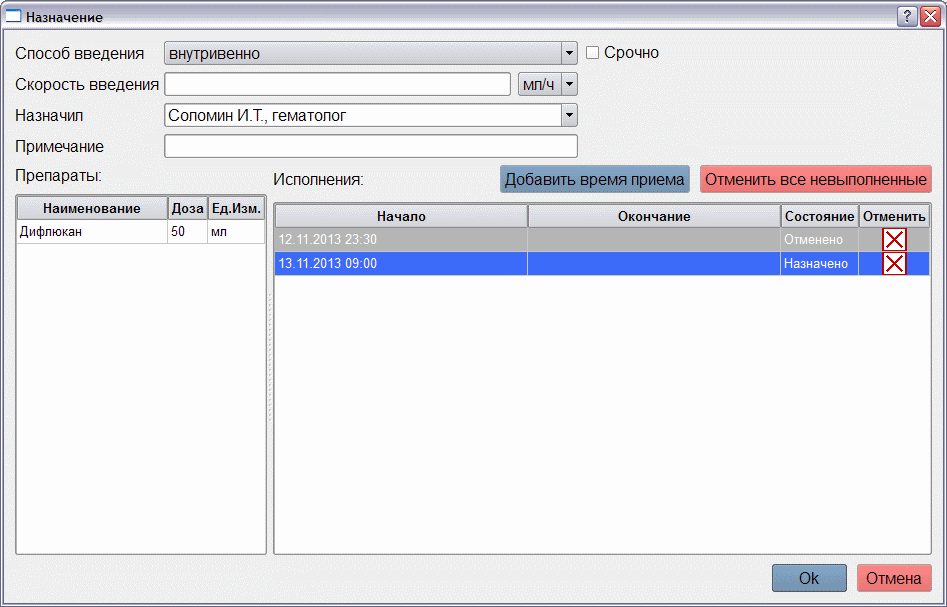
\includegraphics[width = 0.8\textwidth ,keepaspectratio]{st_obr_lnnazn3}
   \caption{Редактирование карточки назначения}
   \label{img_st_obr_lnnazn3}
\end{figure} 

\textbf{Способ Б:}
\begin{enumerate}
 \item Нажать кнопку \btn{Лист назначений} в разделе \dm{Лечение} карточки стационарного обращения.
 \item В основной части листа назначений выбрать нужное время приема для соответствующего назначения и щелкнуть по нему правой кнопкой мыши.
 \item В появившемся контекстном меню выбрать пункт \dm{Редактировать}. Откроется новое окно (Рисунок \ref{img_st_obr_lnnazn4}).
 \item В открывшемся окне нажать кнопку \btn{Отменить}.
 \item При необходимости добавить комментарий в поле \dm{Заметка}.
 \item Нажать кнопку \btn{OK}.
 \item Нажать кнопку \btn{Сохранить} листа назначений.
\end{enumerate}

\begin{figure}[ht]\centering
   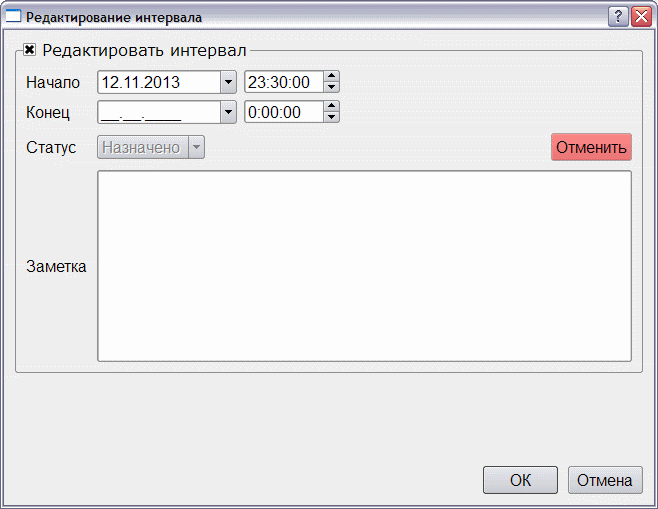
\includegraphics[width = 0.5\textwidth ,keepaspectratio]{st_obr_lnnazn4}
   \caption{Изменение состояния времени приема}
   \label{img_st_obr_lnnazn4}
\end{figure} 

\subsubsection{Печать медицинских документов пациента}

Любой из зарегистрированных медицинских документов (результаты осмотра, направления, результаты исследований и т.д.) можно вывести на печать. Вызвать печать документа можно двумя способами:
\begin{enumerate}
 \item Перейти в соответствующий раздел карточки обращения, щелкнуть правой кнопкой мыши по строке с названием документа, который следует напечатать, и в появившемся контекстном меню выбрать пункт \dm{Печать}.
 \item Открыть карточку документа для редактирования или только для чтения и нажать кнопку \btn{Печать}  в правом нижнем углу окна.
\end{enumerate}
 
Если для выбранного типа документа предусмотрена только одна печатная форма, то откроется окно предварительного просмотра печати документа (Рисунок \ref{img_st_obr_mdprn}). Если же для документа существует несколько печатных форм, то откроется дополнительное меню, где следует выбрать из списка название нужной печатной формы и щелкнуть по нему левой кнопкой мыши, после чего так же откроется окно предварительного просмотра печати (Рисунок \ref{img_st_obr_mdprn}). Внешний вид печатных форм определяется локальными настройками \tmis~и может отличаться в различных ЛПУ.

\begin{figure}[ht]\centering
   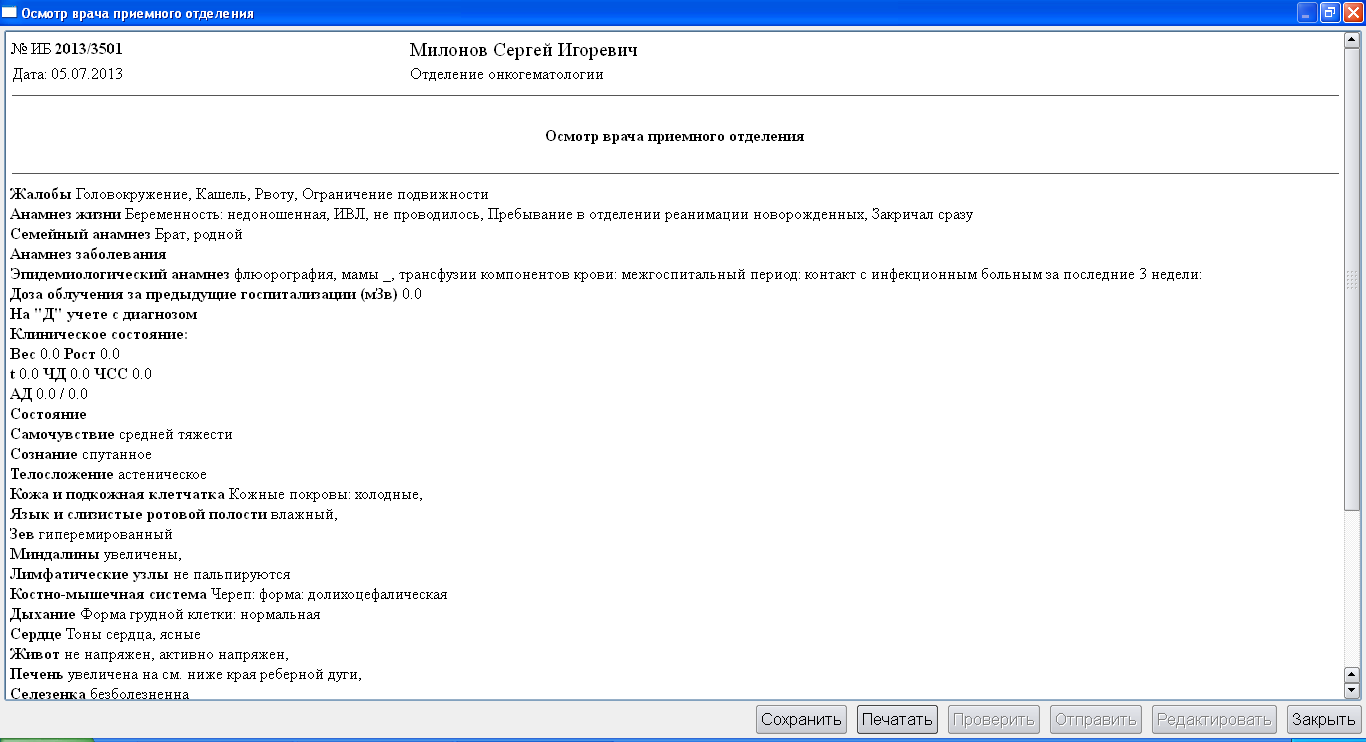
\includegraphics[width = 1\textwidth ,keepaspectratio]{st_obr_mdprn}
   \caption{Окно предварительного просмотра печати медицинского документа}
   \label{img_st_obr_mdprn}
\end{figure} 

Для отправки документа на принтер нужно нажать кнопку \btn{Печатать} .
В \tmis~существует так же возможность печати нескольких медицинских документов одного обращения одновременно. Для этого необходимо перейти в раздел \dm{Основная информация} карточки обращения и нажать кнопку \btn{Печать}, в раскрывшемся меню выбрать название формы, которую следует напечатать и щелкнуть по ней левой кнопкой мыши. Откроется окно предварительного просмотра печатной формы. Для отправки документа на принтер следует нажать кнопку \btn{Печатать}. Внешний вид печатных форм и состав меню данной категории определяется локальными настройками \tmis. Данным способ печати может быть использован, например, для печати всех направлений пациента за текущий день, печати всех результатов осмотров пациента за текущий день, неделю или всю историю болезни и т.д.

\subsection{Закрытие случая обслуживания в стационаре} \label{st_obr_close}

После того как пациент выписан из стационара, его стационарное обращение следует закрыть. Для закрытия обращения необходимо:
\begin{enumerate}
 \item В разделе \dm{Основная информация} заполнить поля \dm{Дата выписки} и \dm{Результат госпитализации}. Дата и время выписки не должны превышать текущие дату и время.
 \item В разделе \dm{Движение пациента} зарегистрировать и перевести в состояние <<Закончено>> действие <<Выписка>>.
 \item В разделе \dm{Медицинские документы} оформить документы <<Выписной эпикриз>> и <<Обоснование клинического диагноза>>.
 \item Рекомендуется перед закрытием обращения перевести все медицинские документы, результаты лабораторных и диагностических исследований в состояние <<Закончено>>.
\end{enumerate}

После выполнения всех вышеперечисленных действий, нужно нажать кнопку \btn{Закрыть обращение}  в левом нижнем углу карточки обращения. Будет выполнена проверка выполнения пунктов 1-4 для текущего обращения. Если возникли замечания по пунктам 1-3, то будет выдано соответствующее сообщение об ошибке и обращение не будет закрыто. Замечания по пункту 4 можно проигнорировать, нажав соответствующую кнопку. Если все проверки пройдены успешно, то обращение закрывается, а на экран выводится соответствующее сообщение (Рисунок \ref{img_st_obr_close}).

\begin{figure}[!ht]\centering
   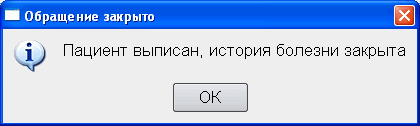
\includegraphics[width = 0.6\textwidth ,keepaspectratio]{st_obr_close}
   \caption{Сообщение об успешном закрытии обращения}
   \label{img_st_obr_close}
\end{figure} 

В течение 2 рабочих дней после закрытия обращение будет доступно для редактирования, после чего редактирование станет невозможно, что аналогично передаче в архив истории болезни пациента.

\subsection{Исполнение назначений}

Для получения списка медикаментозных назначений пациентам отделения на сутки и последующей установки отметок об исполнении назначений постовой или дежурной медсестрой необходимо выбрать пункт меню \mm{Работа \str Лист назначений (исполнения)}. Откроется окно \dm{Лист назначений (исполнения)} (Рисунок \ref{img_st_li}).

В левом верхнем углу окна указывается дата сводного листа назначений. Время начала суточного листа назначений определяется настройками системы. В правом верхнем углу расположена легенда, описывающая окраску строк листа назначений в зависимости от их состояния. В центре сверху расположена область фильтра для назначений. В центральной части окна расположен список всех назначений за указанную дату, отобранных согласно условиям фильтрации. 

\begin{figure}[ht]\centering
   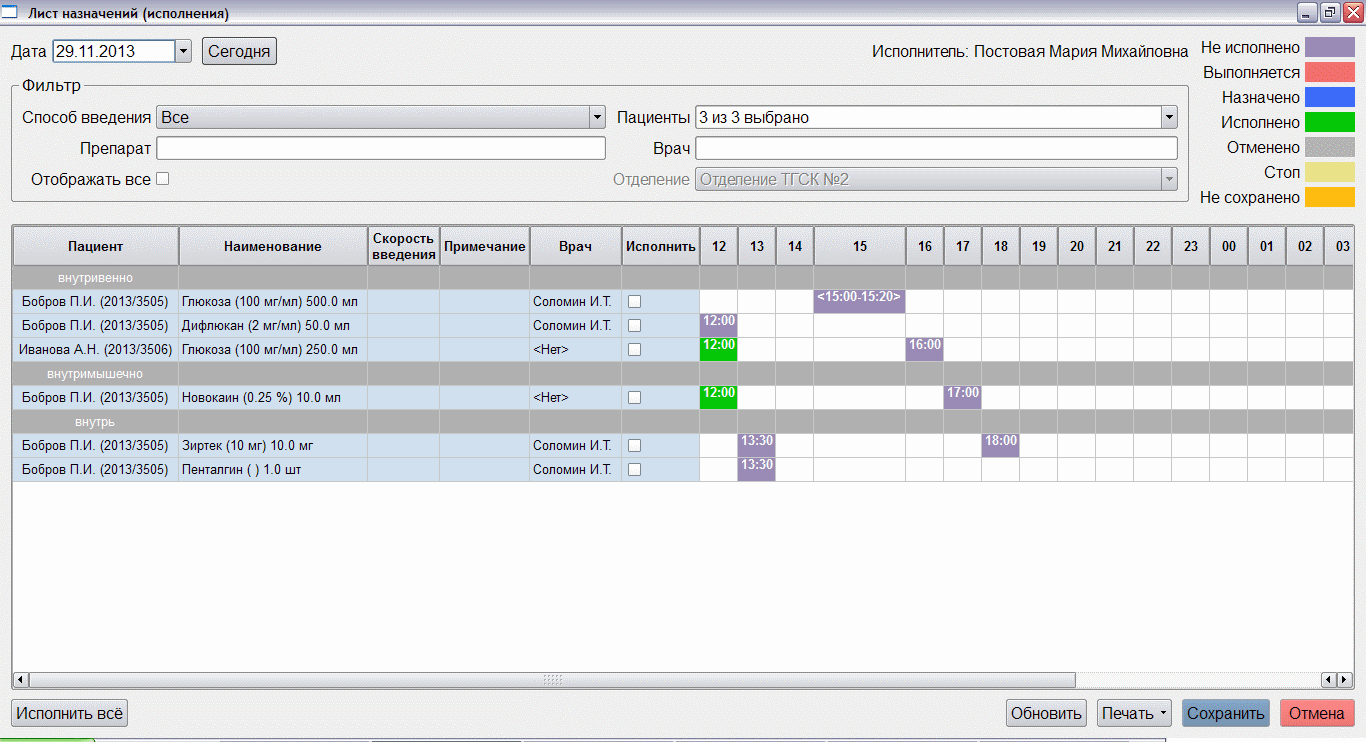
\includegraphics[width = 1\textwidth ,keepaspectratio]{st_li}
   \caption{Лист исполнения назначений}
   \label{img_st_li}
\end{figure} 

Можно просмотреть назначения пациентов на любой день. Для этого нужно установить соответствующую дату в поле \dm{Дата} в левом верхнем углу окна, после чего в основной части окна появится список назначений пациентам отделения на выбранные сутки. При нажатии на кнопку \btn{Сегодня} в поле \dm{Дата} автоматически устанавливается текущая дата. 

Фильтрация назначений возможна по следующим критериям:
\begin{itemize}
 \item \dm{Способ введения} – значение выбирается из списка. Если в данном поле выбрано какое-либо значение, то отображаются назначения только с данным способом введения. Если поле  не заполнено, то отображаются назначения со всеми способами введения. Список способов введения ограничивается теми способами, которые были назначены выбранным пациентам.
 \item \dm{Препарат} – при указании в данном поле наименования либо части наименования препарата, будут отображаться только назначения, содержащие данный препарат или препараты, содержащие в своем наименовании указанное буквосочетание.
 \item Флажок \dm{Отображать все} позволяет включить в список для просмотра назначения, для которых не назначено времен выполнения за выбранные сутки.
 \item \dm{Пациенты} – в свернутом состоянии в поле указывается количество выбранных на текущий момент пациентов. При раскрытии списка отображается список пациентов отделения, слева от фамилий которых можно проставить флажки для выбора. Состояние выбора пациентов перед закрытием окна \dm{Лист назначений (исполнения)} сохраняется и при последующем обращении к листу исполнений, будут открыты назначения ранее выбранных пациентов. Далее, в процессе работы с формой, список выбранных пациентов можно менять сколь угодно раз.
 \item \dm{Врач} – если в поле указана фамилия или часть фамилии врача, то отображаются только назначения, сделанные врачами, в фамилии которых встречается указанное буквосочетание.
 \item \dm{Отделение} – выбирается из дерева структуры ЛПУ. Для работников отделения, это поле недоступно для редактирования. В нем автоматически устанавливается отделение, к которому прикреплен сотрудник. В списке назначений отображаются назначения только указанного отделения.
\end{itemize}
 
Все параметры фильтрации связаны между собой по <<И>>, т.е. назначение попадет в список, если для него будут выполняться ВСЕ условия фильтрации.

При первом открытии листа исполнения список назначений окажется пустым, т.к. для отображения назначений требуется выбрать пациентов в поле \dm{Пациенты} области фильтрации. В последующем, при открытии листа исполнений будет отображаться список назначений пациентов, выбранных в предыдущий раз.

\begin{vnim}
 Необходимо контролировать список выбранных пациентов в листе назначений (исполнения) и своевременно добавлять в него вновь поступивших пациентов
\end{vnim}
 
Список назначений в данном окне содержит фамилию пациента, фамилию назначившего врача, наименование препарата и дозу, скорость введения, примечание. Далее указываются ячейки, соответствующие каждому часу выбранных суток. Информация о назначении размещается в ячейке (или нескольких ячейках), соответствующих времени приема. Периоды приема закрашиваются разным цветом в зависимости от их текущего состояния. Легенда по  цветам назначений находится в правом верхнем углу.

\begin{vnim}
 Все интервалы времени суточного листа назначений, как правило, не умещаются на экране. Для просмотра всего периода назначений следует пользоваться горизонтальной полосой прокрутки
\end{vnim}

Для получения информации о новых назначениях, появившихся с момента открытия листа исполнения следует нажать кнопку \btn{Обновить}  в нижней части окна.

Для отметки об исполнении назначения нужно дважды щелкнуть левой кнопкой мыши по соответствующему интервалу времени приема либо установить флажок в графе \dm{Исполнить} соответствующего назначения. Если исполнение данного назначения возможно в данный момент времени, то цвет периода приема поменяется на зеленый.

При двойном щелчке на определенном интервале времени приема, ставится отметка об исполнении только для данного интервала. При установке флажка \dm{Исполнено} в определенной строке, ставятся отметки об исполнении для всех назначений данной строки, доступных для исполнения на текущий момент.

Можно установить отметки исполнения сразу по всем доступным для исполнения назначениям. Для этого следует нажать на кнопку \btn{Исполнить все}, расположенную в левом нижнем углу окна. После нажатия кнопки флажок \dm{Исполнено} будет установлен во всех строках листа исполнения и, все доступные для исполнения назначения поменяют цвет на зеленый. В качестве исполнителя всех отмеченных назначений будет указан пользователь, под именем которого был выполнен вход в систему.

Доступными для исполнения являются назначения, находящиеся в состоянии <<Не исполнено>> (фиолетового цвета), время редактирования периода (определяется настройками системы и, как правило, составляет 24 часа) которых НЕ истекло.

\begin{prim}
 До тех пор пока отметки об исполнении назначений не будут сохранены, т.е. пока не нажата кнопка \btn{Сохранить} в окне листа исполнений, можно снять отметку об исполнении какого-либо времени выполнения, дважды щелкнув по нему левой кнопкой мыши, либо отказаться от установки отметок об исполнении для какого-либо назначения, сняв флажок в ячейке \dm{Исполнено} для указанной строки.
\end{prim}
 
После того как все отметки об исполнении назначений сделаны, необходимо сохранить их. Для этого нужно нажать кнопку \btn{Сохранить} в правом нижнем углу. После этого отмена исполнения становится невозможной.

\subsubsection{Печать листа назначений (исполнения)}

Из окна \mm{Работа \str Лист назначений (исполнения)} возможна печать сводного листа назначений по всем пациентам отделения за указанные сутки и печать листа назначений одного из пациентов.

Перед печатью листа назначений необходимо указать сутки, за которые необходимо напечатать лист, в поле \dm{Дата}. Далее следует нажать кнопку \btn{Печать} в правом нижнем углу окна и в появившемся меню выбрать соответствующий вариант печати. При выборе пункта меню \dm{Лист назначений (исполнений)} будет производиться печать листа назначений по всем пациентам отделения, для которых за выбранные сутки назначены периоды исполнения назначений. При выборе пункта меню \dm{Лист назначений (исполнений)} с указанием в скобках фамилии пациента, будет печататься лист назначений только по соответствующему пациенту.

\begin{figure}[!ht]\centering
   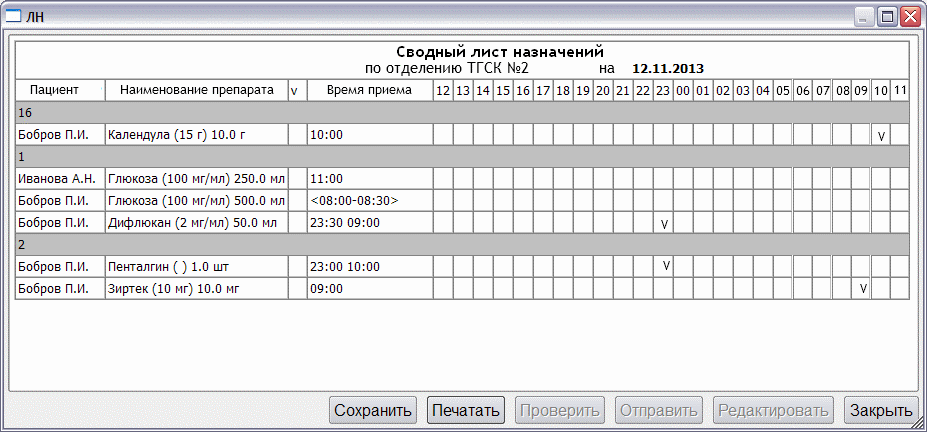
\includegraphics[width = 1\textwidth ,keepaspectratio]{st_li_prn}
   \caption{Окно предварительного просмотра печати листа назначений}
   \label{img_st_li_prn}
\end{figure} 

После выбора вида печати листа назначения откроется окно предварительного просмотра печати (Рисунок \ref{img_st_li_prn}). Чтобы отправить лист назначения на принтер, необходимо нажать кнопку \btn{Печатать}. Для сохранения печатной формы в файл следует нажать кнопку \btn{Сохранить} и в открывшемся диалоговом окне указать имя и тип файла для сохранения. Для выхода из окна предварительного просмотра нужно нажать кнопку \btn{Закрыть}.


%\subsection{Формирование сводки по движению пациентов}

%\subsubsection{Формирование листа ежедневного учета движения пациентов (Ф. 007/У)}

%Для формирования ежедневного листа движения пациентов по заданному отделению необходимо в главном меню выбрать \mm{Анализ \str Стационар \str Форма 007У}. В открывшемся окне следует указать параметры отчета (Рисунок \ref{img_st_rep_par}):
%\begin{itemize}
% \item \dm{Дата отчета} – дата, на которую формируется листок движения. По умолчанию выбирается предыдущая дата.
% \item \dm{Подразделение} – отделение, для которого формируется сводка. Необходимо в дереве структуры ЛПУ выбирать отделение, к которому привязаны койки.
% \item \dm{Режим койки} – можно выбрать тип коек для учета (только круглосуточные, либо только не круглосуточные). По умолчанию в сводку попадают все койки, а для параметра установлено значение <<не учитывать>>.
% \item \dm{Начало рабочего дня} – время начала суток, принятое в ЛПУ для отчетности.
%\end{itemize}

%\begin{figure}[ht]\centering
%   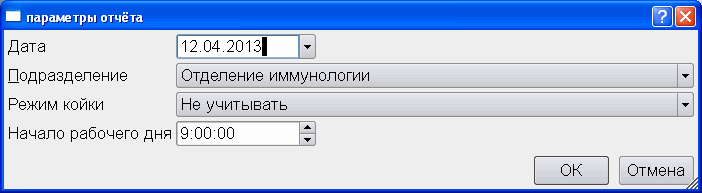
\includegraphics[width = 0.7\textwidth ,keepaspectratio]{st_rep_par}
%   \caption{Параметры формирования листа движения пациентов (Ф. 007)}
%   \label{img_st_rep_par}
%\end{figure} 

%После того, как все параметры заполнены, необходимо нажать кнопку \btn{OK} и подождать некоторое время, пока на экране появится окно предварительного просмотра печатной формы отчета Ф. 007/У (Рисунок \ref{img_st_rep007_1} - \ref{img_st_rep007_2}). Для отправки сводки на печать необходимо в открывшемся окне нажать кнопку \btn{Печатать}. Для сохранения полученных результатов в файл следует нажать кнопку \btn{Сохранить} и в появившемся окне указать папку для сохранения файла, имя файла, выбрать тип файла (поддерживаются форматы PDF, HTML, ODT и PS) и нажать кнопку \btn{Сохранить}.

%\begin{figure}[ht]\centering
%   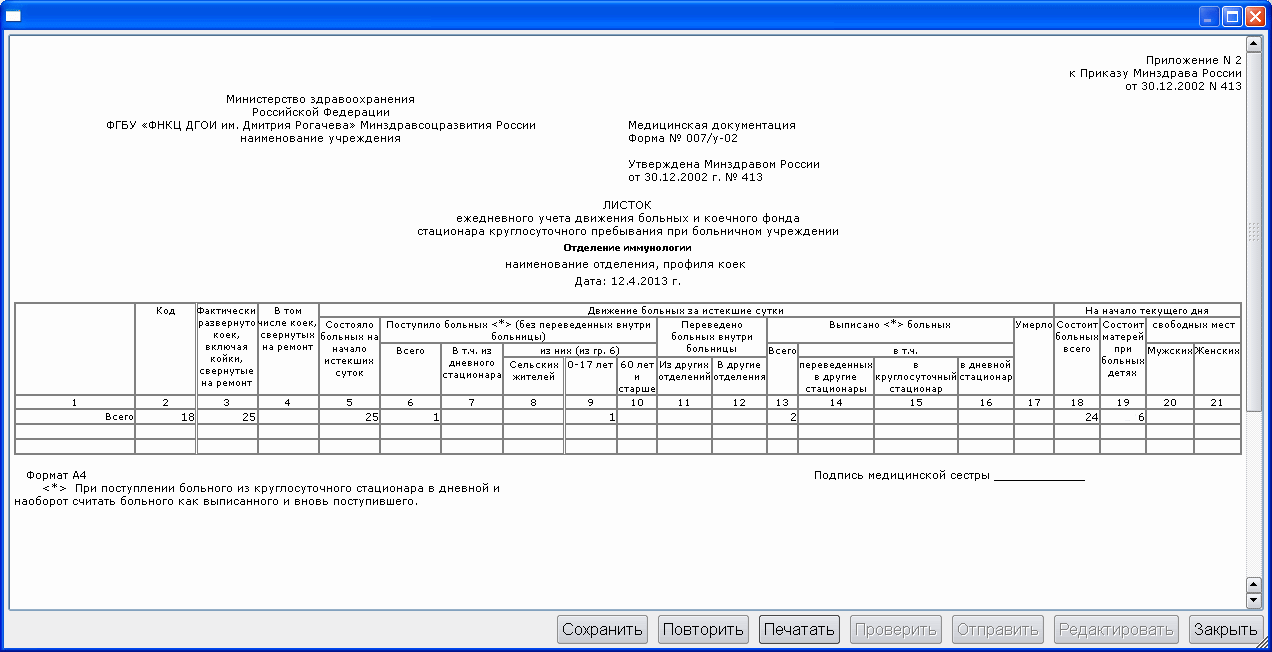
\includegraphics[width = 1\textwidth ,keepaspectratio]{st_rep007_1}
%   \caption{Ф. 007/У (лицевая сторона)}
%   \label{img_st_rep007_1}
%\end{figure} 

%\begin{figure}[ht]\centering
%   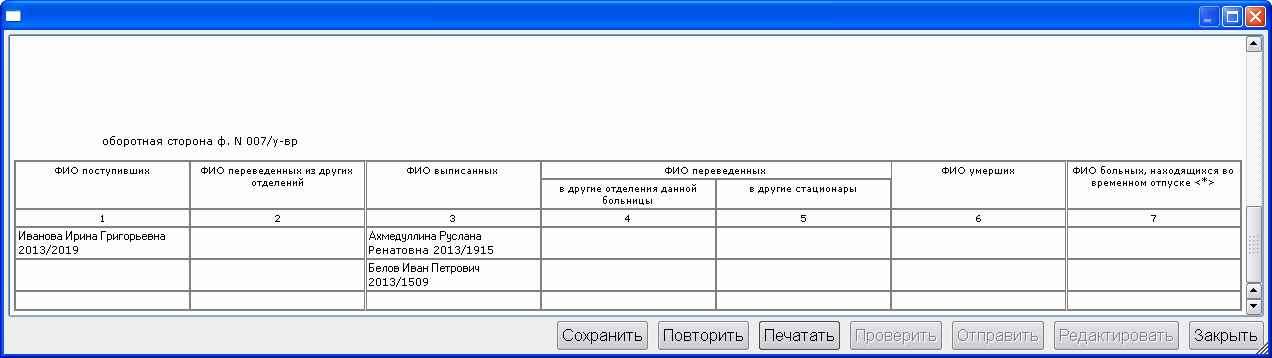
\includegraphics[width = 1\textwidth ,keepaspectratio]{st_rep007_2}
%   \caption{Ф. 007/У продолжение (оборотная сторона)}
%   \label{img_st_rep007_2}
%\end{figure}

%При нажатии кнопки \btn{Повторить} осуществляется возврат к окну задания параметров сводки, что позволяет сформировать сводку заново с другими параметрами.

%\subsubsection{Формирование сводной ведомости по движению пациентов}

%Для формирования сводной ведомости учета движения пациентов за год необходимо в главном меню выбрать пункт \mm{Анализ \str Стационар \str Форма 016}. В открывшемся окне следует указать параметры формирования отчета (Рисунок \ref{img_st_rep_par2}):
%\begin{itemize}
% \item \dm{Год} – год, за который формируется сводка.
% \item \dm{Подразделение} – необходимо в дереве структуры ЛПУ выбрать отделение ЛПУ, к которому привязаны койки, либо одну из вышестоящих структурных единиц. Для формирования сводки по всему ЛПУ следует выбрать название ЛПУ.
% \item \dm{Профиль койки} – при выборе значения в данном поле сводка будет сформирована только по койкам выбранного профиля. По умолчанию в поле установлено значение <<не задано>> и сводка формируется по всем профилям коек.
%\end{itemize}
 

%\begin{figure}[ht]\centering
%   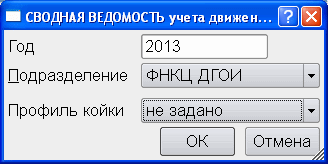
\includegraphics[width = 0.6\textwidth ,keepaspectratio]{st_rep_par2}
%   \caption{Параметры формирования сводной ведомости по движению}
%   \label{img_st_rep_par2}
%\end{figure} 

%После того, как все параметры формирования сводки указаны, необходимо нажать кнопку \btn{OK}  и дождаться формирования отчета (Рисунок \ref{img_st_rep016}).

%\begin{figure}[ht]\centering
%   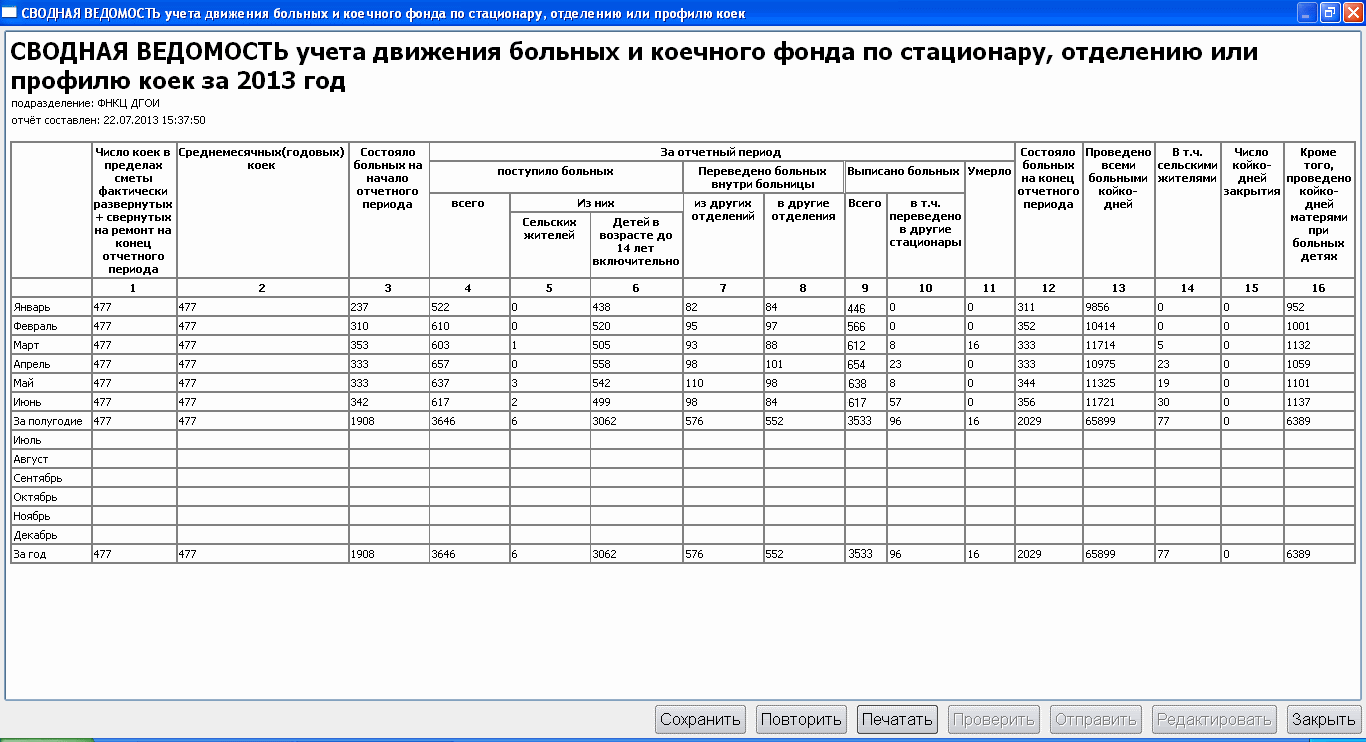
\includegraphics[width = 1\textwidth ,keepaspectratio]{st_rep016}
%   \caption{Окно предварительного просмотра печати сводной ведомости}
%   \label{img_st_rep016}
%\end{figure}

%\begin{vnim}
% Формирование сводки за  год может занять продолжительное время.
%\end{vnim}
 
%Для отправки сводки на печать необходимо в открывшемся окне нажать кнопку \btn{Печатать}. Для сохранения полученных результатов в файл следует нажать кнопку \btn{Сохранить} и в появившемся окне указать папку для сохранения файла, имя файла, выбрать тип файла (поддерживаются форматы PDF, HTML, ODT и PS) и нажать кнопку \btn{Сохранить}.

\subsection{Стационарный монитор} \label{st_mon}

Стационарный монитор имеет очень широкую область применения. Он может использоваться для следующих задач:
\begin{itemize}
 \item Получение информации о состоянии коечного фонда ЛПУ или отдельно взятого подразделения;
 \item Получение информации о наличии свободных коек в отделении;
 \item Назначение диетпитания пациентам;
 \item Просмотр списка поступивших пациентов, очереди на госпитализацию;
 \item Просмотр списка пациентов, находящихся в ЛПУ или выбранном подразделении, и состава их обращений; 
 \item Просмотр списка пациентов, переведенных в другие отделения за  выбранный период;
 \item Просмотр списка готовых к выписке, выписанных, умерших пациентов, списки отказов от госпитализации;
 \item Вывод на печать списков пациентов, сформированных по различным критериям;
 \item Просмотр списка вновь поступивших пациентов и печать <<Журнала учета госпитализаций>> (Ф.001/У).
\end{itemize}
 
Для запуска стационарного монитора нужно в главном меню выбрать пункт \mm{Работа \str Стационарный монитор}. Окно стационарного монитора состоит из следующих функциональных частей (Рисунок \ref{img_st_mon}):
\begin{itemize}
 \item В секции 1 находится дерево структуры ЛПУ. При выборе подразделения в дереве, отображаются данные только по указанному подразделению. При установке курсора на корень дерева, отображаются сведения по всему ЛПУ. Изменения состава данных происходит при каждом перемещении курсора по дереву, т.е. нажатия дополнительных кнопок для применения фильтра по подразделению не требуется. В связи с этим могут наблюдаться небольшие задержки при перемещении курсора по дереву ЛПУ.
 \item В секции 2 расположена панель фильтрации данных. Доступность определенных полей фильтра изменяется в зависимости от выбранной вкладки в секции 4. В верхней части панели расположены поля для фильтрации коек, в нижней – для фильтрации обращений.
 \item В секции 3 расположены функциональные кнопки. Их доступность зависит от позиции курсора в секции 4.
 \item В секции 4 находится область данных, содержащая несколько вкладок. Состав информации отображаемой в области данных определяется выбранной вкладкой, позицией курсора в секции 1 и параметрами фильтрации, указанными в секции 2.
 \item Секция 5 содержит кнопку \btn{Печать}, которая позволяет вывести данные секции 4 в определенном виде на принтер, и кнопку \btn{Закрыть}, которая служит для закрытия окна стационарного монитора.
\end{itemize}

\begin{figure}[ht]\centering
   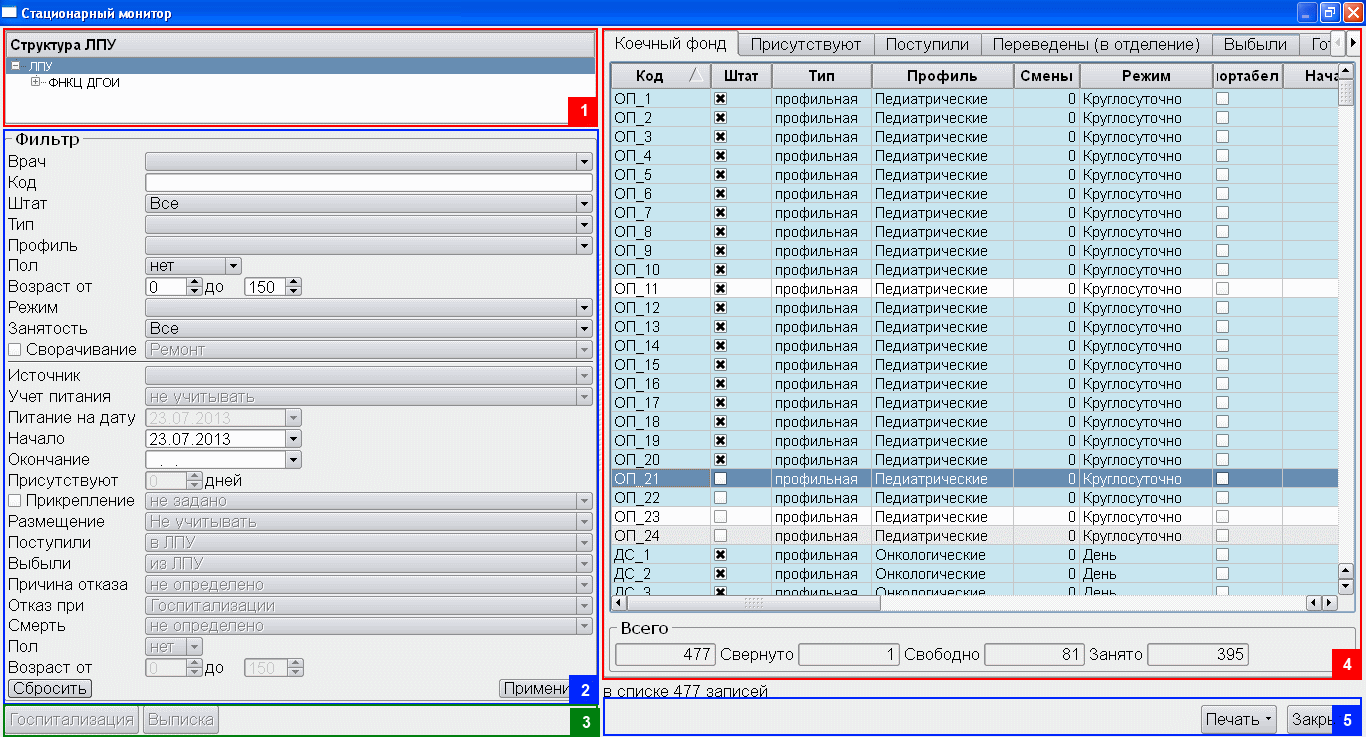
\includegraphics[width = 1\textwidth ,keepaspectratio]{st_mon}
   \caption{Стационарный монитор. Общий вид окна}
   \label{img_st_mon}
\end{figure}

\subsubsection{Сведения о коечном фонде}

Для получения сведений о коечном фонде необходимо в секции 4 выбрать вкладку \dm{Коечный фонд} (Рисунок \ref{img_st_mon}). Свободные койки в списке отображаются белым или серым цветом, занятые – голубым.

Состав списка зависит от подразделения, выбранного в секции 1 и от параметров фильтрации, заданных в секции 2. Фильтрация в данном случае возможна по следующим параметрам:
\begin{itemize}
 \item \dm{Код} – код койки. Код необходимо вводить с клавиатуры полностью, фильтрация по части кода не реализована.
 \item \dm{Штат} – может принимать 3 значения: <<Да>> = только штатные койки, <<Нет>> = только заштатные койки, <<Все>> = все койки;
 \item \dm{Тип койки} выбирается из списка;
 \item \dm{Профиль койки} выбирается из списка;
 \item \dm{Пол} – позволяет отобрать койки, на которых возможно размещение только пациентов выбранного пола.
 \item \dm{Возраст} – указывается интервал возрастов пациентов для размещения на койке.
 \item \dm{Режим} работы койки выбирается из списка: <<Круглосуточная>>, <<День>>, <<Ночь>>, <<Утро>>, <<Вечер>>. Если режим не задан, то выбираются все койки.
 \item \dm{Занятость} койки выбирается из списка. Можно выбрать только свободные, только занятые, занятые транспортабельными больными, свободные или транспортабельные койки отдельно.
 \item Установка флажка \dm{Сворачивание} позволяет отобрать только свернутые койки. При этом необходимо выбрать из списка справа причину сворачивания. В список попадут только койки, свернутые по выбранной причине.
\end{itemize}
 
После того, как все параметры фильтрации заданы, необходимо нажать кнопку \btn{Применить}, после чего данные в секции 4 будут отфильтрованы согласно указанным условиям. Параметры фильтра связаны между собой по <<И>>. Т.е. в результаты фильтрации попадут только койки, для которых выполнены все заданные условия.

При нажатии на кнопку \btn{Сбросить}, отображаются все койки подразделения, выбранного в секции 1.

Из данного окна можно просмотреть обращение пациента, размещенного на выбранной койке. Для этого следует щелкнуть правой кнопкой мыши и в появившемся меню выбрать пункт \dm{Открыть обращение}. В открывшемся окне (Рисунок \ref{img_st_mon_obr}) будет показана краткая информация об обращении, дважды щелкнув по ней левой кнопкой мыши, можно открыть карточку обращения.

\begin{figure}[ht]\centering
   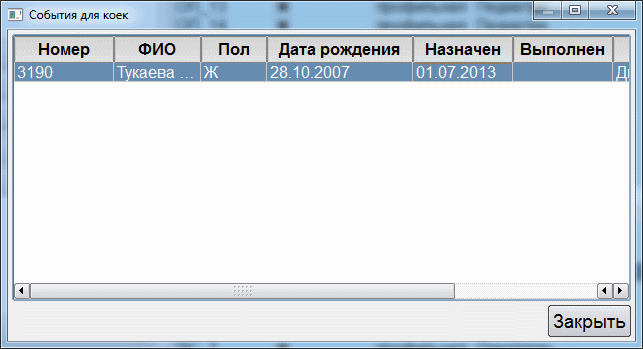
\includegraphics[width = 0.6\textwidth ,keepaspectratio]{st_mon_obr}
   \caption{Обращение пациента, размещенного на койке}
   \label{img_st_mon_obr}
\end{figure}

Для печати сводного отчета по коечному фонду необходимо нажать кнопку \btn{Печать} в секции 5 и в появившемся меню выбрать пункт \dm{Сводка}. На экране появится окно предварительного просмотра печатной формы сводного отчета по коечному фонду с разбивкой по подразделениям, профилю и занятости (Рисунок \ref{img_st_mon_prn}).

\begin{vnim}
 При формировании печатной формы сводки на данные налагаются условия фильтрации и выбранного подразделения. Т.е. в сводку попадают только койки, которые отображаются в момент вызова печати в секции 4.
\end{vnim}

Полученный отчет можно отправить на печать нажатием кнопки \btn{Печатать}  или сохранить в файл нажатием кнопки \btn{Сохранить} в окне предварительного просмотра.

\begin{figure}[ht]\centering
   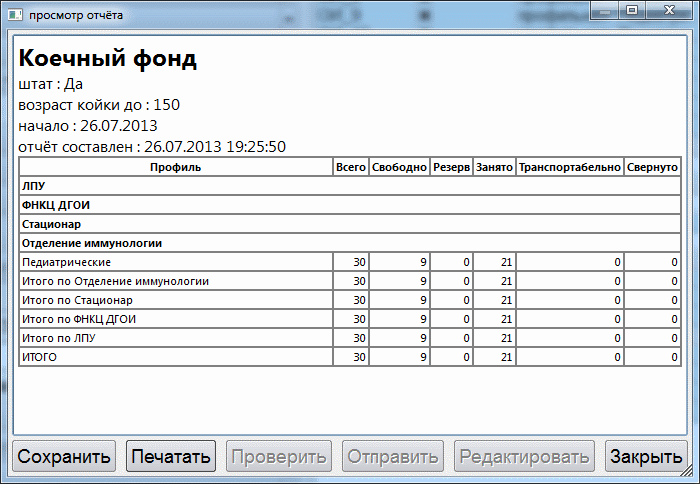
\includegraphics[width = 0.6\textwidth ,keepaspectratio]{st_mon_prn}
   \caption{Предварительный просмотр сводки по коечному фонду}
   \label{img_st_mon_prn}
\end{figure}

\subsubsection{Сведения о присутствующих пациентах}

В данном разделе (Рисунок \ref{img_st_mon_pris}) можно просмотреть информацию о пациентах, находящихся в текущий момент на госпитализации в ЛПУ или выбранном отделении в зависимости от положения курсора в дереве структуры ЛПУ (Рисунок \ref{img_st_mon}, секция 1).

\begin{figure}[ht]\centering
   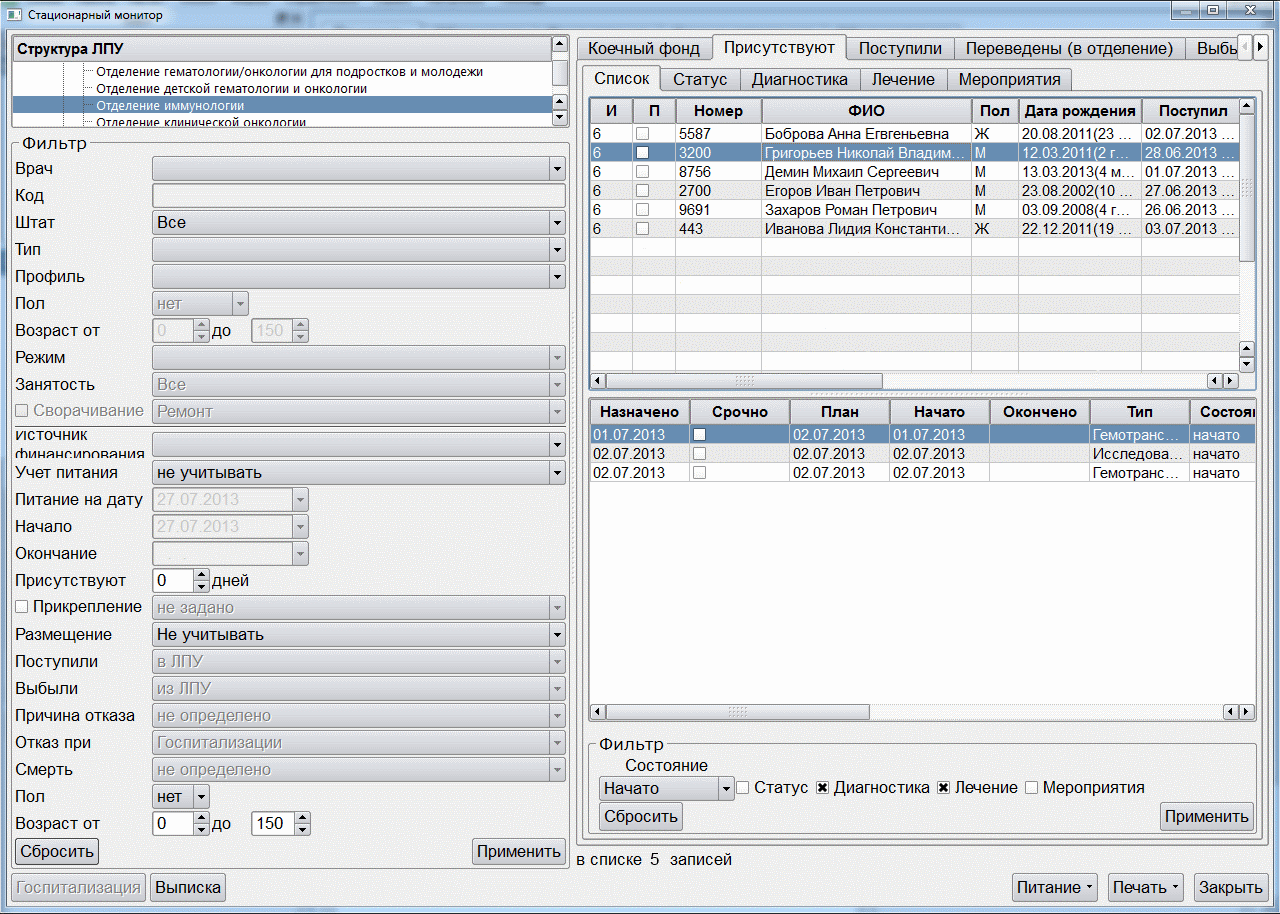
\includegraphics[width = 1\textwidth ,keepaspectratio]{st_mon_pris}
   \caption{Стационарный монитор. Вкладка <<Присутствуют>>}
   \label{img_st_mon_pris}
\end{figure}

Фильтрация списка обращений возможна по следующим критериям:
\begin{itemize}
 \item \dm{Врач} – выбирается из списка. Позволяет выбрать пациентов, находящихся на лечении у выбранного врача.
 \item \dm{Штат} – позволяет отфильтровать пациентов по расположению на койках: <<Да>> = только пациенты, размещенные на штатных койках, <<Нет>> = только пациенты, размещенные на заштатных койках, <<Все>> = все пациенты;
 \item \dm{Тип} койки, на которой размещен пациент, выбирается из списка;
 \item \dm{Профиль} койки, на которой размещен пациент, выбирается из списка;
 \item \dm{Источник финансирования} обращения выбирается из списка;
 \item \dm{Учет питания} – позволяет отобрать пациентов, для которых назначено или не назначено питание;
 \item \dm{Питание на дату} – дата, на которую следует рассматривать наличие назначения питания. Заполняется, если в предыдущем поле выбрано учитывать (<<назначено>> или <<не назначено>>).
 \item \dm{Присутствуют} – указывается продолжительность госпитализации в днях. Производится отбор пациентов только с указанной продолжительностью госпитализации.
 \item \dm{Прикрепление} – при установке данного флажка требуется выбрать тип прикрепления из списка.
 \item \dm{Размещение} – при выборе значения <<Да>> производится отбор только размещенных на койках пациентов; при выборе значения <<Нет>> - только неразмещенных. По умолчанию отображаются все пациенты, а в поле указано значение <<не учитывать>>.
 \item \dm{Пол} – позволяет отобрать пациентов определенного пола;
 \item \dm{Возраст} – указывается интервал возрастов пациентов для отбора.
\end{itemize}
 
После того, как параметры фильтрации заданы, необходимо нажать кнопку \btn{Применить}, после чего список обращений будет отфильтрован согласно указанным условиям. Параметры фильтра связаны между собой по <<И>>. Т.е. в результаты фильтрации попадут только обращения, для которых выполнены все заданные условия.

При нажатии на кнопку \btn{Сбросить}, отображаются все открытые обращения подразделения, выбранного в секции 1.

Область данных в текущем представлении разбита на несколько вкладок. На вкладке \dm{Список} в верхней части области данных отображается список обращений пациентов, находящихся в текущий момент на госпитализации, в средней части – список медицинских документов, содержащихся в выбранном в верхней части окна обращении. Состав отображаемых медицинских документов определяется настройками фильтра в нижней части области данных. Документы могут быть отфильтрованы по типу и состоянию. По умолчанию отображаются все лечебные мероприятия, лабораторные и диагностические исследования  в состоянии <<Начато>>. Состояние выбирается из списка, для отображения типа медицинских документов, необходимо установить флажок \putx~рядом с его названием в фильтре. После изменения настроек фильтра необходимо нажать кнопку \btn{Применить} в правом нижнем углу экрана. Нажатие кнопки \btn{Сбросить} возвращает настройки фильтра в состояние по умолчанию.

Следующие 4 вкладки содержат списки медицинских документов различных типов, входящих в состав обращений, отображенных на вкладке \dm{Список} в соответствии с условиями фильтрации. Ниже приведена таблица соответствия размещения документов на вкладках текущего раздела стационарного монитора и карточки обращения.

{\small
\begin{tabular}{|p{7cm}|p{8.5cm}|}
\hline
\textbf{Название вкладки в стационарном мониторе} & \textbf{Название раздела в карточке обращения} \\
\hline
Статус & Медицинские документы \\
\hline
Диагностика &	Диагностические и лабораторные исследования \\
\hline
Лечение & Лечение \\
\hline
Мероприятия &	Движение пациента \\
\hline
\end{tabular}
}
\vspace*{0.5em}

Для каждой из вкладок в нижней части окна существует фильтр, позволяющий отобрать документы соответствующей группы по состоянию и типу. По умолчанию отбираются документы всех типов в состоянии <<Начато>>. Тип документа выбирается из списка. После изменения параметров фильтрации, требуется нажать кнопку \btn{Применить} в правом нижнем углу экрана. Нажатие кнопки \btn{Сбросить}  возвращает настройки фильтра в состояние по умолчанию.

Из данной вкладки можно открыть карточку обращения пациента. Для этого следует выбрать обращение на вкладке \dm{Список} и дважды щелкнуть по нему левой кнопкой мыши либо щелкнуть по выбранной записи правой кнопкой мыши и в появившемся меню выбрать пункт \dm{Открыть обращение}.

Список пациентов, находящихся в стационаре, можно вывести на печать. Для этого нужно нажать кнопку \btn{Печать} в правом нижнем углу окна и в появившемся меню выбрать пункт \dm{Сводка}. На экране появится окно предварительного просмотра печатной формы списка пациентов (Рисунок \ref{img_st_mon_prn2}).

\begin{figure}[ht]\centering
   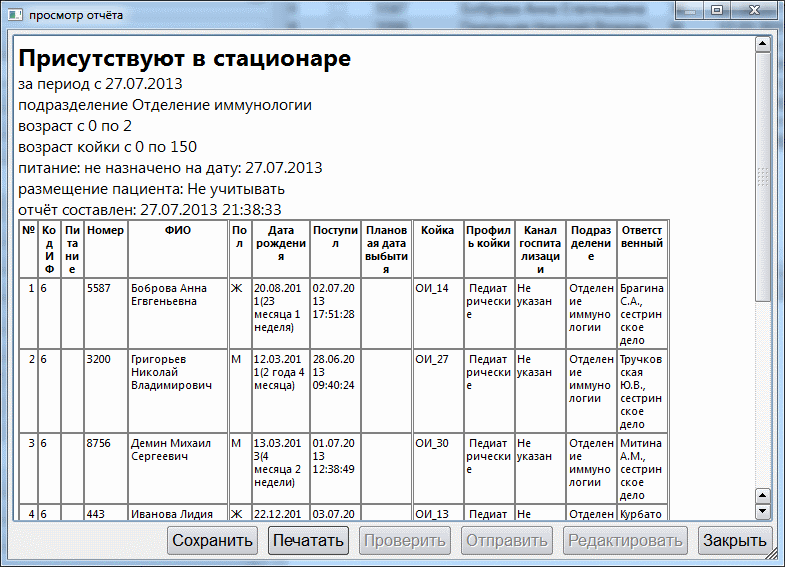
\includegraphics[width = 0.7\textwidth ,keepaspectratio]{st_mon_prn2}
   \caption{Предварительный просмотр печати списка пациентов, присутствующих в стационаре}
   \label{img_st_mon_prn2}
\end{figure}
 
\begin{vnim}
 При формировании печатной формы сводки на данные налагаются условия фильтрации и выбранного подразделения. Т.е. в список попадают только пациенты, обращения которых отображаются на вкладке \dm{Список} в момент вызова печати.
\end{vnim}
 
Полученный отчет можно отправить на печать нажатием кнопки \btn{Печатать}  или сохранить в файл нажатием кнопки \btn{Сохранить} в окне предварительного просмотра.

\subsubsection{Назначение питания пациентам}

На вкладке \dm{Присутствуют} стационарного монитора можно так же выполнить назначение диетпитания пациентам, находящимся в стационаре. Для этого нужно найти пациента на вкладке \dm{Список}, щелкнуть по его фамилии правой кнопкой мыши и в появившемся контекстном меню выбрать пункт \dm{Назначить питание по шаблону} либо нажать кнопку \btn{Питание} в правом нижнем углу окна и в появившемся меню выбрать аналогичный пункт. В открывшемся окне (Рисунок \ref{img_st_mon_eat}) необходимо указать период дат назначения питания, установить флажок \dm{Обновить} (чтобы изменить ранее назначенный шаблон, если он был), выбрать шаблон питания, щелкнув по нему левой кнопкой мыши и нажать кнопку \btn{Выбрать}. После этого у выбранного пациента появится отметка о наличии шаблона питания на указанную дату в колонке \dm{П} списка обращений. Для просмотра информации о составе шаблонов питания, следует в окне выбора шаблона питания (Рисунок \ref{img_st_mon_eat}) выбрать шаблон и нажать кнопку \btn{Просмотр}. Откроется окно просмотра состава шаблона.

\begin{figure}[ht]\centering
   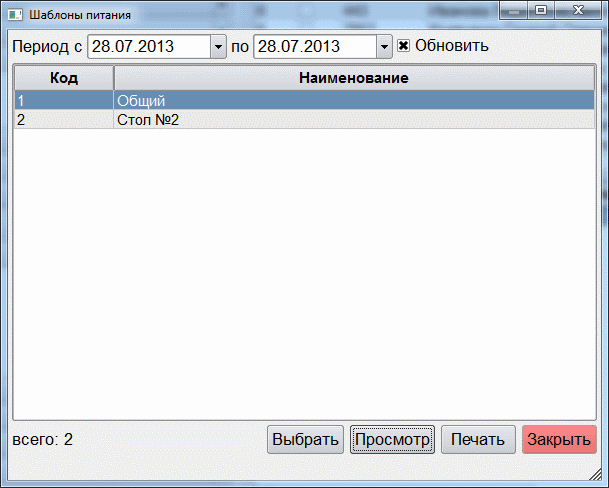
\includegraphics[width = 0.6\textwidth ,keepaspectratio]{st_mon_eat}
   \caption{Окно выбора шаблона питания}
   \label{img_st_mon_eat}
\end{figure}

С помощью кнопки \btn{Питание}  можно так же:
\begin{itemize}
 \item Выделить всех пациентов, для которых назначено питание на указанную дату;
 \item Выделить всех пациентов, для которых НЕ назначено питание на указанную дату;
 \item Выделить всех пациентов;
 \item Снять выделение;
 \item Выполнить пролонгацию питания.
\end{itemize}
 
Для этого нужно нажать кнопку \btn{Питание} в правом нижнем углу окна и в появившемся меню выбрать соответствующий пункт.

Для вывода на печать порционного требования на указанную дату нужно нажать кнопку \btn{Печать}  в правом нижнем углу окна и в появившемся меню выбрать \dm{Порционник}. Откроется окно предварительного просмотра печати порционного требования. Для отправки на принтер следует нажать кнопку \btn{Печатать} , для сохранения в файл – кнопку \btn{Сохранить}.

\subsubsection{Список поступивших пациентов}

На вкладке \dm{Поступили} стационарного монитора можно просмотреть список пациентов, поступивших в ЛПУ или отделение за выбранный период (Рисунок \ref{img_st_mon_new}).

\begin{figure}[ht]\centering
   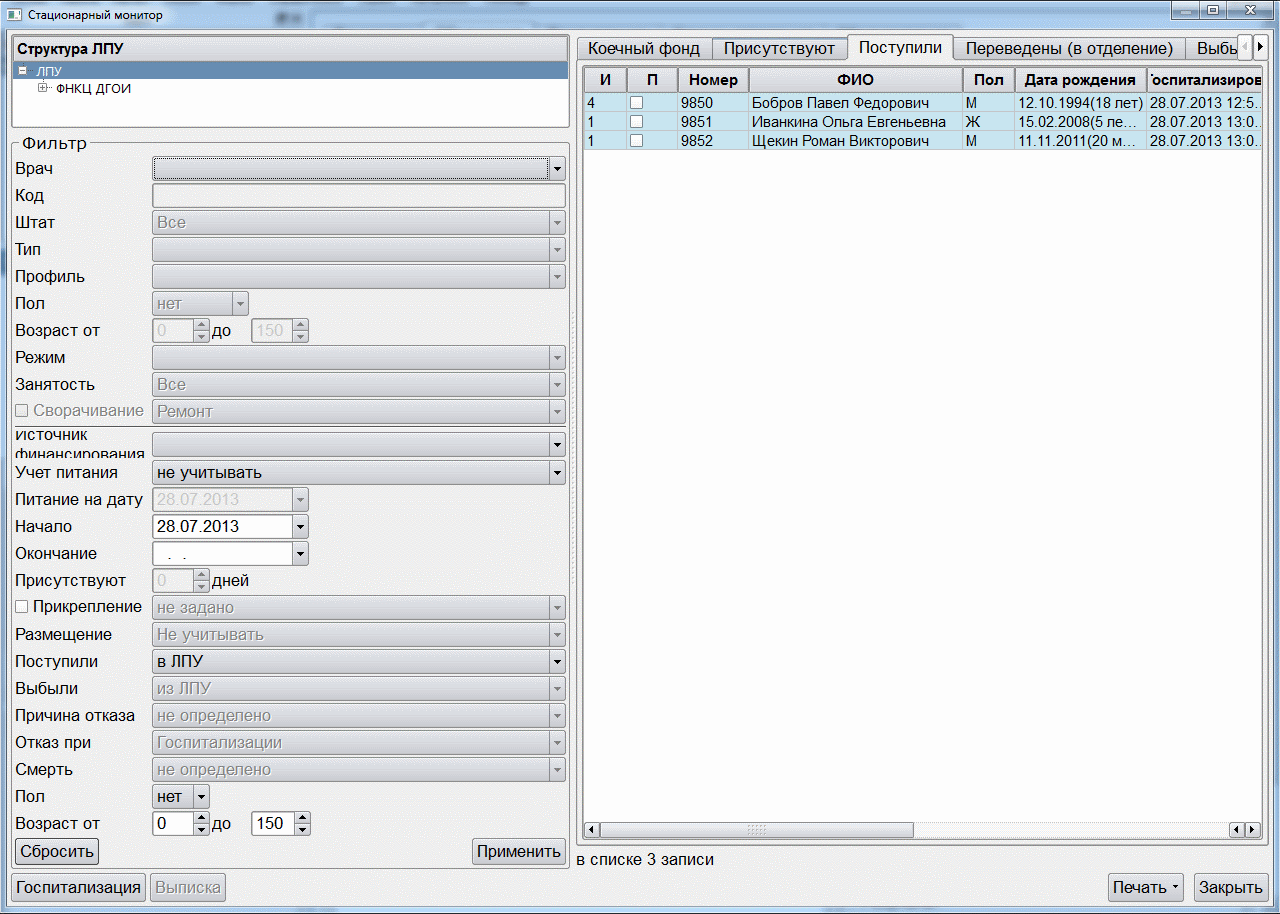
\includegraphics[width = 1\textwidth ,keepaspectratio]{st_mon_new}
   \caption{Стационарный монитор. Вкладка <<Поступили>>}
   \label{img_st_mon_new}
\end{figure}

Если в левом верхнем углу окна, в дереве структуры ЛПУ выбрано какое-либо подразделение, то отображаются только пациенты, направленные при поступлении в выбранное отделение. По умолчанию (при выборе в дереве структуры значения <<ЛПУ>>) отображаются все пациенты, поступившие в ЛПУ.

Фильтрация списка поступивших пациентов возможна по следующим параметрам:
\begin{itemize}
 \item \dm{Врач} – выбирается из списка. Позволяет выбрать пациентов, для которых в качестве лечащего врача в обращении указан выбранный врач.
 \item \dm{Источник финансирования} обращения выбирается из списка;
 \item \dm{Учет питания} – позволяет отобрать пациентов, для которых назначено или не назначено питание;
 \item \dm{Питание на дату} – дата, на которую следует рассматривать наличие назначения питания. Заполняется, если в предыдущем поле выбрано учитывать (<<назначено>> или <<не назначено>>).
 \item \dm{Начало} – дата начала заданного периода для отбора.
 \item \dm{Окончание} – дата окончания заданного периода для отбора.
 \item \dm{Прикрепление} – при установке данного флажка требуется выбрать тип прикрепления из списка.
 \item \dm{Поступили} – выбирается из списка: <<в ЛПУ>>, <<в приемное отделение>>, <<в отделение>>. При выборе последнего варианта, в фильтре становятся доступны дополнительные параметры, касающиеся размещения пациента на койке: \dm{Штат}, \dm{Тип}, \dm{Профиль} койки, \dm{Размещение}.
 \item \dm{Пол} – позволяет отобрать пациентов определенного пола;
 \item \dm{Возраст} – позволяет отобрать пациентов определенной возрастной группы.
\end{itemize}
 
После заполнения параметров фильтра следует нажать кнопку \btn{Применить}, данные в секции 4 изменятся в соответствии с настройками фильтра. Для возврата к настройкам фильтра по умолчанию нужно нажать кнопку \btn{Сбросить}.

Из данной вкладки можно открыть карточку обращения пациента. Для этого нужно дважды щелкнуть левой кнопкой мыши по фамилии выбранного пациента либо щелкнуть правой кнопкой мыши по фамилии выбранного пациента и в появившемся контекстном меню выбрать пункт \dm{Открыть обращение}.

При нажатии кнопки \btn{Печать}, расположенной в правом нижнем углу окна, можно выбрать в появившемся меню пункт \dm{Сводка}. В результате откроется окно предварительного просмотра печати списка пациентов, отображаемого в текущий момент в области данных стационарного монитора (Рисунок \ref{img_st_mon_prn3}).

\begin{figure}[ht]\centering
   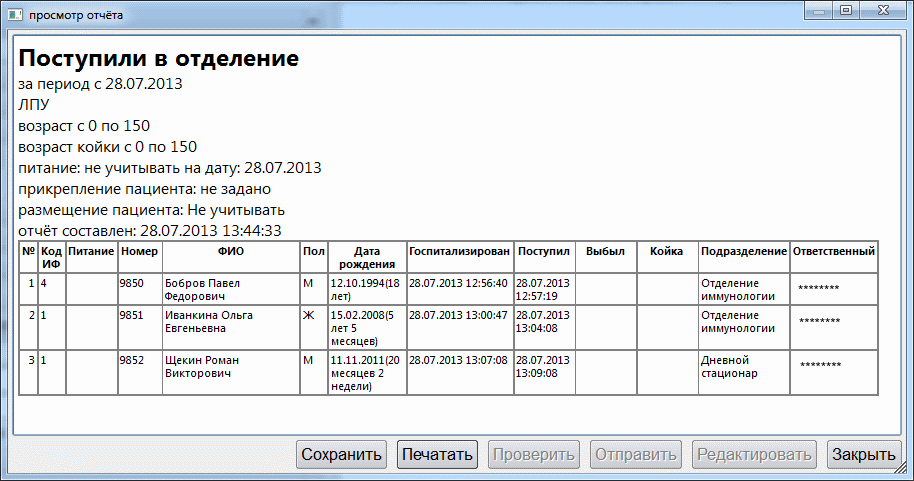
\includegraphics[width = 0.8\textwidth ,keepaspectratio]{st_mon_prn3}
   \caption{Предварительный просмотр печати списка поступивших пациентов}
   \label{img_st_mon_prn3}
\end{figure}

Полученный отчет можно отправить на печать нажатием кнопки \btn{Печатать}  или сохранить в файл нажатием кнопки  \btn{Сохранить} в окне предварительного просмотра.

\subsubsection{Печать <<Журнала учёта приёма больных и отказов в госпитализации>> (Ф. 001/У)}

Для печати журнала приемного отделения требуется на вкладке \dm{Поступили} стационарного монитора отобрать пациентов за требуемый период с помощью фильтра и нажать кнопку \btn{Печать}  в правом нижнем углу окна и в появившемся меню выбрать \dm{Журнал}. Откроется окно предварительного просмотра печати журнала (Рисунок \ref{img_st_mon_prn001}).

\begin{figure}[ht]\centering
   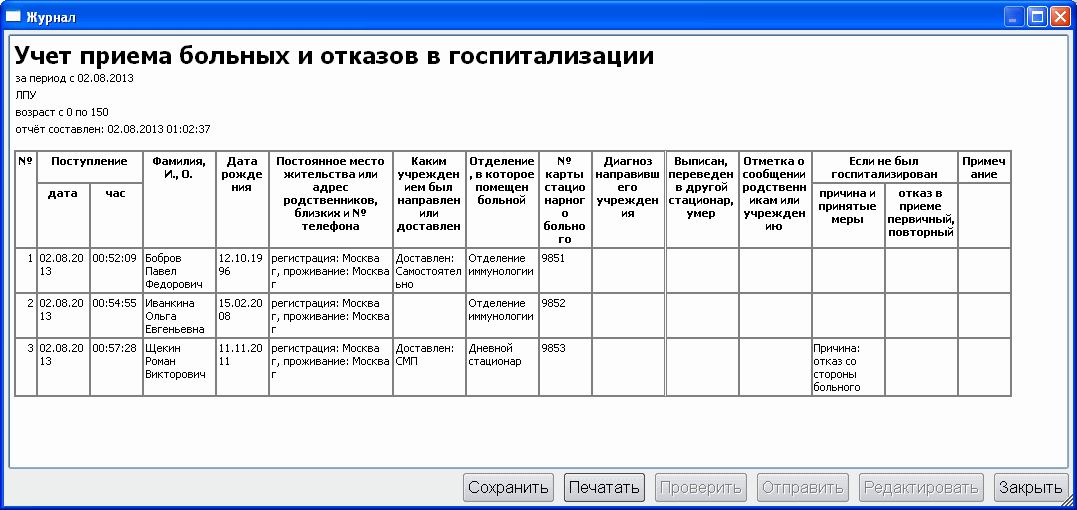
\includegraphics[width = 1\textwidth ,keepaspectratio]{st_mon_prn001}
   \caption{Журнал учета приема больных и отказов в госпитализации (ф. 001/У)}
   \label{img_st_mon_prn001}
\end{figure}

Для отправки журнала на печать нужно нажать кнопку  \btn{Печатать}, для сохранения данных в файл необходимо нажать кнопку  \btn{Сохранить} в окне предварительного просмотра, а затем указать папку для сохранения файла, имя и тип файла.

\subsubsection{Список пациентов, переведенных в отделение}

В данном разделе отображается список пациентов, которые переводились из одного отделения в другое за указанный период (Рисунок \ref{img_st_mon_perev}).

\begin{figure}[ht]\centering
   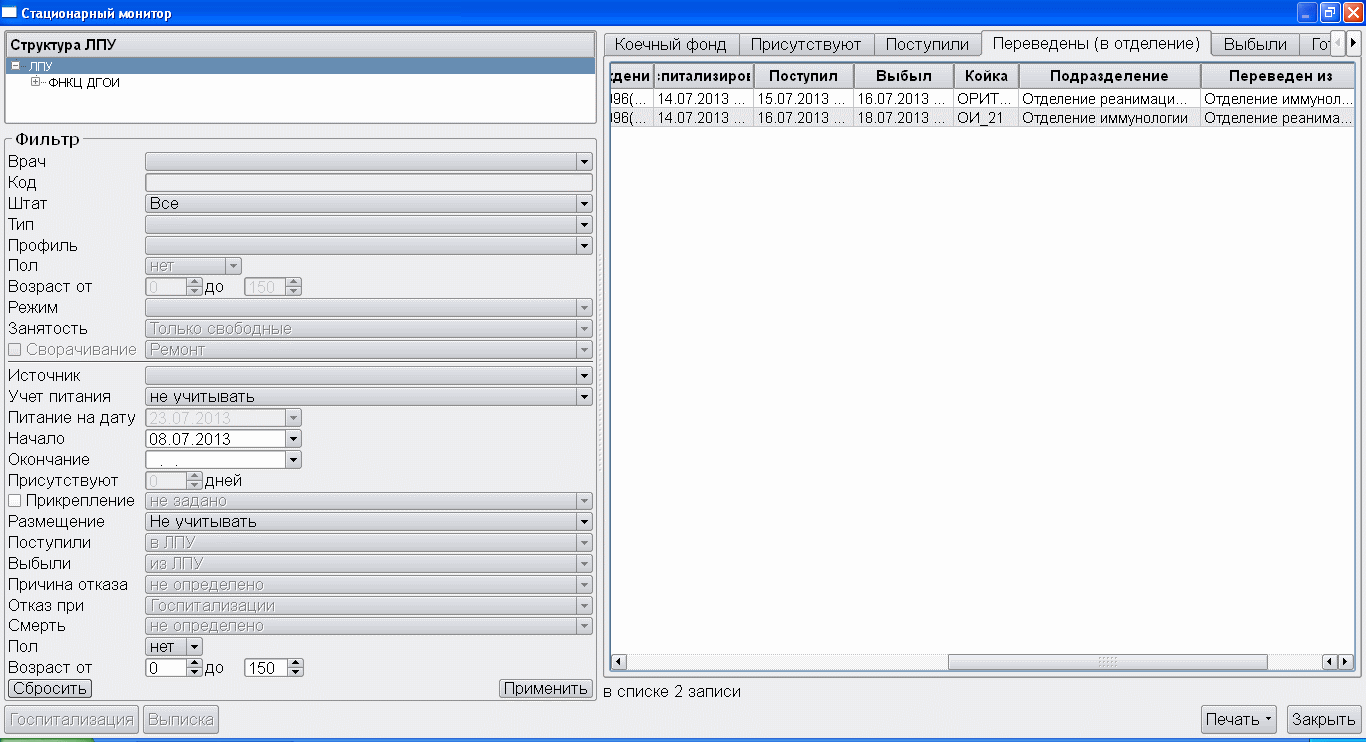
\includegraphics[width = 1\textwidth ,keepaspectratio]{st_mon_perev}
   \caption{Стационарный монитор. Вкладка <<Переведены (в отделение)>>}
   \label{img_st_mon_perev}
\end{figure}

Фильтрация списка переведенных пациентов возможна по следующим критериям:
\begin{itemize}
 \item \dm{Врач} – выбирается из списка. Позволяет выбрать пациентов, находящихся на лечении у выбранного врача.
 \item \dm{Штат} – позволяет отфильтровать пациентов по расположению на койках: <<Да>> = только пациенты, размещенные на штатных койках, <<Нет>> = только пациенты, размещенные на заштатных койках, <<Все>> = все пациенты;
 \item \dm{Тип} койки, на которой размещен пациент, выбирается из списка;
 \item \dm{Профиль} койки, на которой размещен пациент, выбирается из списка;
 \item \dm{Источник финансирования} обращения выбирается из списка;
 \item \dm{Учет питания} – позволяет отобрать пациентов, для которых назначено или не назначено питание;
 \item \dm{Питание на дату} – дата, на которую следует рассматривать наличие назначения питания. Заполняется, если в предыдущем поле выбрано учитывать (<<назначено>> или <<не назначено>>).
 \item \dm{Начало} – дата начала периода для отбора переводов.
 \item \dm{Окончание} – дата окончания периода для отбора переводов.
 \item \dm{Прикрепление} – при установке данного флажка требуется выбрать тип прикрепления из списка.
 \item \dm{Размещение} – при выборе значения <<Да>> производится отбор только размещенных на койках пациентов; при выборе значения <<Нет>> - только неразмещенных. По умолчанию отображаются все пациенты, а в поле указано значение <<не учитывать>>.
 \item \dm{Пол} – позволяет отобрать пациентов определенного пола;
 \item \dm{Возраст} – указывается интервал возрастов пациентов для отбора.
\end{itemize}
 
После того, как параметры фильтрации заданы, необходимо нажать кнопку \btn{Применить}, после чего список переведенных пациентов за указанный период будет отфильтрован согласно указанным условиям. Параметры фильтра связаны между собой по <<И>>. Т.е. в результаты фильтрации попадут только обращения, для которых выполнены все заданные условия.

При нажатии на кнопку \btn{Сбросить}, параметры фильтрации возвращаются к настройкам по умолчанию.

Можно вывести на печать список пациентов, отображаемых в текущий момент в области данных. Для этого нужно нажать кнопку \btn{Печать}  в правом нижнем углу окна и в появившемся окне выбрать пункт \dm{Сводка}. Откроется окно предварительного просмотра списка переведенных пациентов. Для отправки документа на принтер, необходимо нажать кнопку \btn{Печатать}  в окне предварительного просмотра печати, для сохранения списка в файл – кнопку \btn{Сохранить}.

Для открытия карточки обращения переведенного пациента следует дважды щелкнуть по фамилии пациента в списке левой кнопкой мыши либо щелкнуть по соответствующей строке в списке правой кнопкой мыши и в появившемся меню выбрать пункт \dm{Открыть обращение}.

\subsubsection{Список выбывших пациентов}

На данной вкладке отображается список пациентов, выбывших из ЛПУ за указанный период (Рисунок \ref{img_st_mon_vib}). Если в дереве структуры ЛПУ выбрано какое-либо подразделение, то отображается список выбывших пациентов из этого подразделения.

\begin{figure}[ht]\centering
   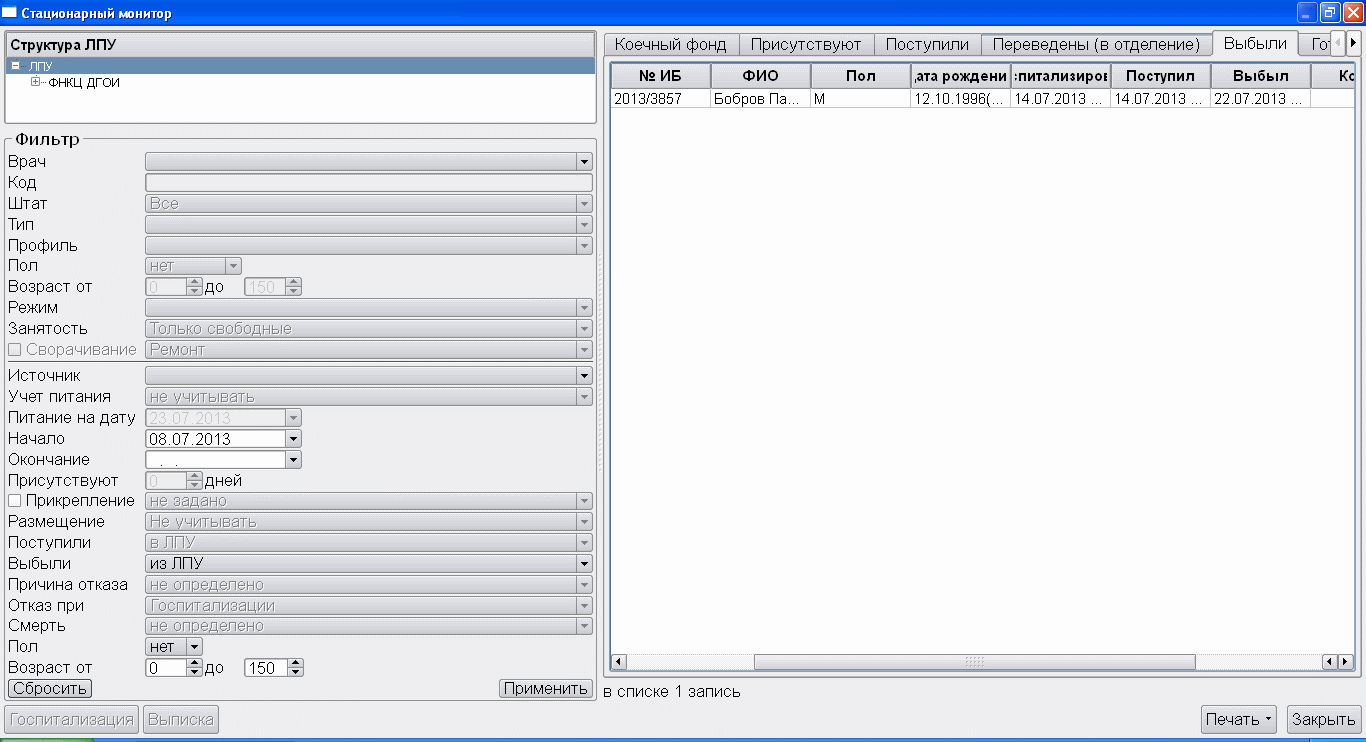
\includegraphics[width = 1\textwidth ,keepaspectratio]{st_mon_vib}
   \caption{Стационарный монитор. Вкладка <<Выбывшие>>}
   \label{img_st_mon_vib}
\end{figure}

Для данной вкладки возможно задать следующие параметры фильтрации:
\begin{itemize}
 \item \dm{Врач} – лечащий врач пациента при выписке.
 \item \dm{Источник финансирования} обращения выбирается из списка.
 \item \dm{Начало} – дата начала периода выбытия для отбора.
 \item \dm{Окончание} – дата окончания периода выбытия для отбора.
 \item \dm{Прикрепление} – при установке данного флажка следует выбрать из списка справа тип прикрепления для отбора.
 \item \dm{Выбыли} – может принимать 2 значения: <<из ЛПУ>> – в результат выборки попадают пациенты, выписанные из ЛПУ за указанный период; при выборе значения параметра <<из отделений>> в список добавляются пациенты, которые были переведены в другое отделение в указанном периоде. При выборе второго варианта, становятся доступны дополнительные параметры фильтрации: \dm{Штат}, \dm{Тип}, \dm{Профиль} койки.
 \item \dm{Пол} – выбирается из списка.
 \item \dm{Возраст} – можно задать интервал возрастов выписанных пациентов.
\end{itemize}
 
После того, как все параметры фильтрации заданы, следует нажать кнопку \btn{Применить}, после чего в области данных будет отображен список выписанных пациентов согласно указанным условиям. При нажатии на кнопку \btn{Сбросить}, параметры фильтрации возвращаются к настройкам по умолчанию.

Можно вывести на печать список пациентов, отображаемых в текущий момент в области данных. Для этого нужно нажать кнопку   в правом нижнем углу окна и в появившемся окне выбрать пункт \dm{Сводка}. Откроется окно предварительного просмотра списка переведенных пациентов. Для отправки документа на принтер, необходимо нажать кнопку \btn{Печатать} в окне предварительного просмотра печати, для сохранения списка в файл – кнопку \btn{Сохранить}.

Для открытия карточки обращения выписанного пациента следует дважды щелкнуть по соответствующей строке в списке левой кнопкой мыши либо щелкнуть по ней правой кнопкой мыши и в появившемся контекстном меню выбрать пункт \dm{Открыть обращение}.

\subsubsection{Список пациентов, готовых к выбытию}

Данная вкладка аналогична предыдущей. Здесь можно применить те же параметры фильтрации, так же сформировать список пациентов и вывести его на печать. Но в данном представление выводятся список пациентов, которые еще не выписаны, но их выписка запланирована на указанный период дат (т.е. плановая дата завершения последнего действия <<Движение>> попадает в заданный период).

\subsubsection{Очередь на госпитализацию}

На данной вкладке отображается список пациентов, стоящих в очереди на госпитализацию (Рисунок \ref{img_st_mon_list}). В список попадают пациенты, госпитализация которых запланирована на указанный период.
 
\begin{figure}[ht]\centering
   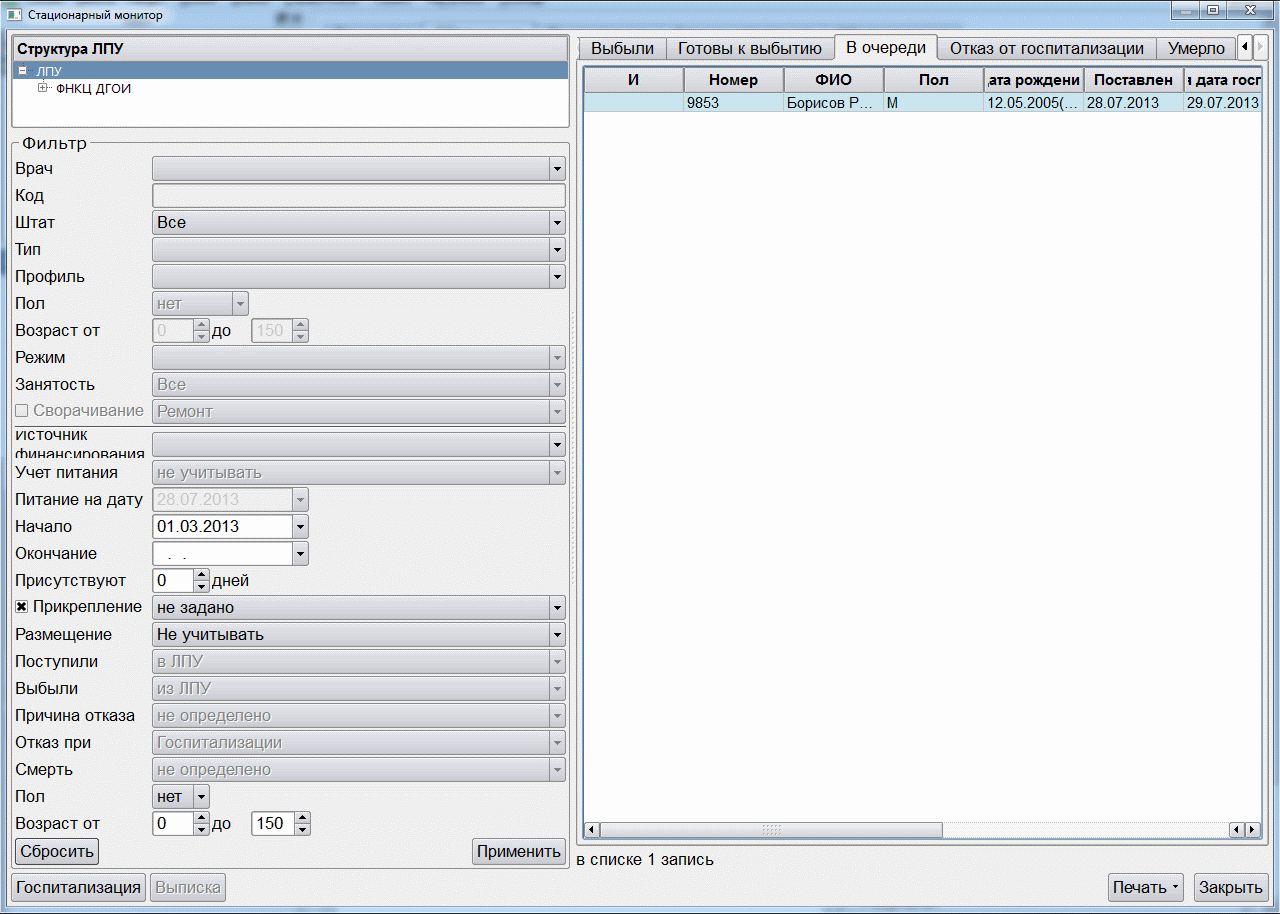
\includegraphics[width = 1\textwidth ,keepaspectratio]{st_mon_list}
   \caption{Стационарный монитор. Вкладка <<В очереди>>}
   \label{img_st_mon_list}
\end{figure}

Выбрав подразделение в дереве структуры ЛПУ, можно просмотреть очередь госпитализации для заданного подразделения.

На данной вкладке возможно применение следующих параметров фильтрации:
\begin{itemize}
 \item \dm{Врач} – поиск обращений, находящихся в очереди по лечащему врачу.
 \item \dm{Штат} – можно отдельно отобрать пациентов, которые запланированы для размещения на штатных и заштатных койках.
 \item \dm{Тип} – выбор типа койки, на которую запланирован пациент из списка.
 \item \dm{Профиль} – выбор профиля койки, на которую запланирован пациент.
 \item \dm{Начало} – дата начала периода для отбора.
 \item \dm{Окончание} – дата окончания периода для отбора.
 \item \dm{Присутствуют} – количество дней ожидания в очереди.
 \item Флажок \dm{Прикрепление} позволяет выполнить отбор по типу прикрепления. Для этого в списке справа следует выбрать тип из списка.
 \item \dm{Размещение} – позволяет отобрать пациентов, которые запланированы на определенную койку (<<Да>>) или для которых в плане не задана конкретная койка (<<Нет>>).
 \item \dm{Пол} – выбор пациентов определенного пола.
 \item \dm{Возраст} – выбор пациентов определенного возраста. Задается начало и конец интервала возраста в годах.
\end{itemize}

Для того чтобы вступили в действие параметры фильтрации, необходимо нажать кнопку \btn{Применить}, после чего в области данных будет отображен список пациентов, находящихся в очереди на госпитализацию, согласно указанным условиям. При нажатии на кнопку \btn{Сбросить}, параметры фильтрации возвращаются к настройкам по умолчанию.

Можно вывести на печать список пациентов, отображаемых в текущий момент в области данных. Для этого нужно нажать кнопку \btn{Печать} в правом нижнем углу окна и в появившемся окне выбрать пункт \dm{Сводка}. Откроется окно предварительного просмотра списка пациентов. Для отправки документа на принтер, необходимо нажать кнопку \btn{Печатать} в окне предварительного просмотра печати, для сохранения списка в файл – кнопку \btn{Сохранить}.

Для открытия карточки обращения пациента, находящегося в очереди на госпитализацию, следует дважды щелкнуть левой кнопкой мыши по соответствующей строке в списке либо щелкнуть по ней правой кнопкой мыши и в появившемся меню выбрать пункт \dm{Открыть обращение}.

\subsubsection{Список отказов от госпитализации}

На данную вкладку попадают пациенты, которым было отказано в госпитализации или сами пациенты отказались от госпитализации при обращении в приемное отделение стационара в указанный период (Рисунок \ref{img_st_mon_otkaz}). На данной вкладке выбор подразделения в дереве структуры ЛПУ не имеет значения.

\begin{figure}[ht]\centering
   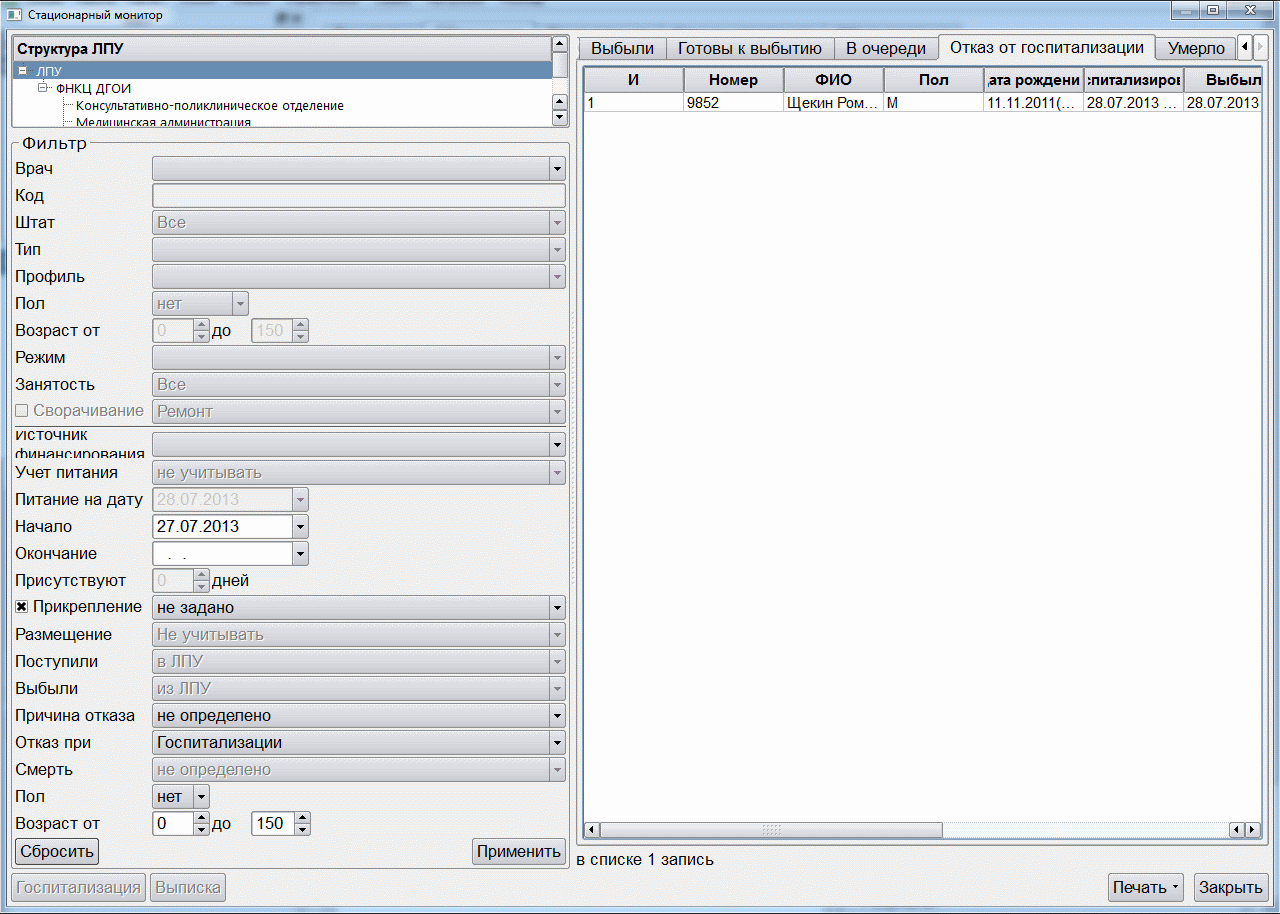
\includegraphics[width = 1\textwidth ,keepaspectratio]{st_mon_otkaz}
   \caption{Стационарный монитор. Вкладка <<Отказ от госпитализации>>}
   \label{img_st_mon_otkaz}
\end{figure}

К списку пациентов, отказавшихся от госпитализации, можно применить следующие параметры фильтрации:
\begin{itemize}
 \item \dm{Врач} – отбираются обращения, где лечащим врачом является выбранный врач. Фактически, отбор осуществляется по врачу, производившему осмотр пациента в приемном отделении.
 \item \dm{Источник финансирования} обращения выбирается из списка.
 \item \dm{Начало} – дата начала периода для отбора.
 \item \dm{Окончание} – дата окончания периода для отбора.
 \item При установке флажка \dm{Прикрепление} следует выбрать тип прикрепления из списка справа.
 \item \dm{Причина отказа} выбирается из списка.
 \item \dm{Отказ при} может принимать 2 значения <<Госпитализации>> или <<Планировании>>.
 \item \dm{Пол} выбирается из списка и позволяет отобрать отказных пациентов определенного пола.
 \item \dm{Возраст} – можно выбрать пациентов определенной возрастной группы, задав соответствующий интервал возрастов в годах.
\end{itemize}

После того, как параметры фильтрации заданы, следует нажать кнопку \btn{Применить}, после чего в области данных будет отображен список отказных пациентов, отобранных согласно указанным условиям. При нажатии на кнопку \btn{Сбросить}, параметры фильтрации возвращаются к настройкам по умолчанию.

В данном представлении возможно вывести на печать <<Журнал отказов в госпитализации>>. В него попадут пациенты, отображаемые в текущий момент в области данных. Для этого нужно нажать кнопку \btn{Печать} в правом нижнем углу окна и в появившемся окне выбрать пункт \dm{Журнал}. Откроется окно предварительного просмотра журнала. Для отправки документа на принтер, необходимо нажать кнопку \btn{Печатать}  в окне предварительного просмотра печати, для сохранения списка в файл – кнопку \btn{Сохранить}.

Для открытия карточки обращения отказного пациента следует дважды щелкнуть левой кнопкой мыши по соответствующей строке в списке либо щелкнуть по ней правой кнопкой мыши и в появившемся контекстном меню выбрать пункт \dm{Открыть обращение}.

\subsubsection{Список умерших пациентов}

На данной вкладке отображаются пациенты, стационарные обращения которых завершились смертью в ЛПУ (Рисунок \ref{img_st_mon_umer}).

\begin{figure}[ht]\centering
   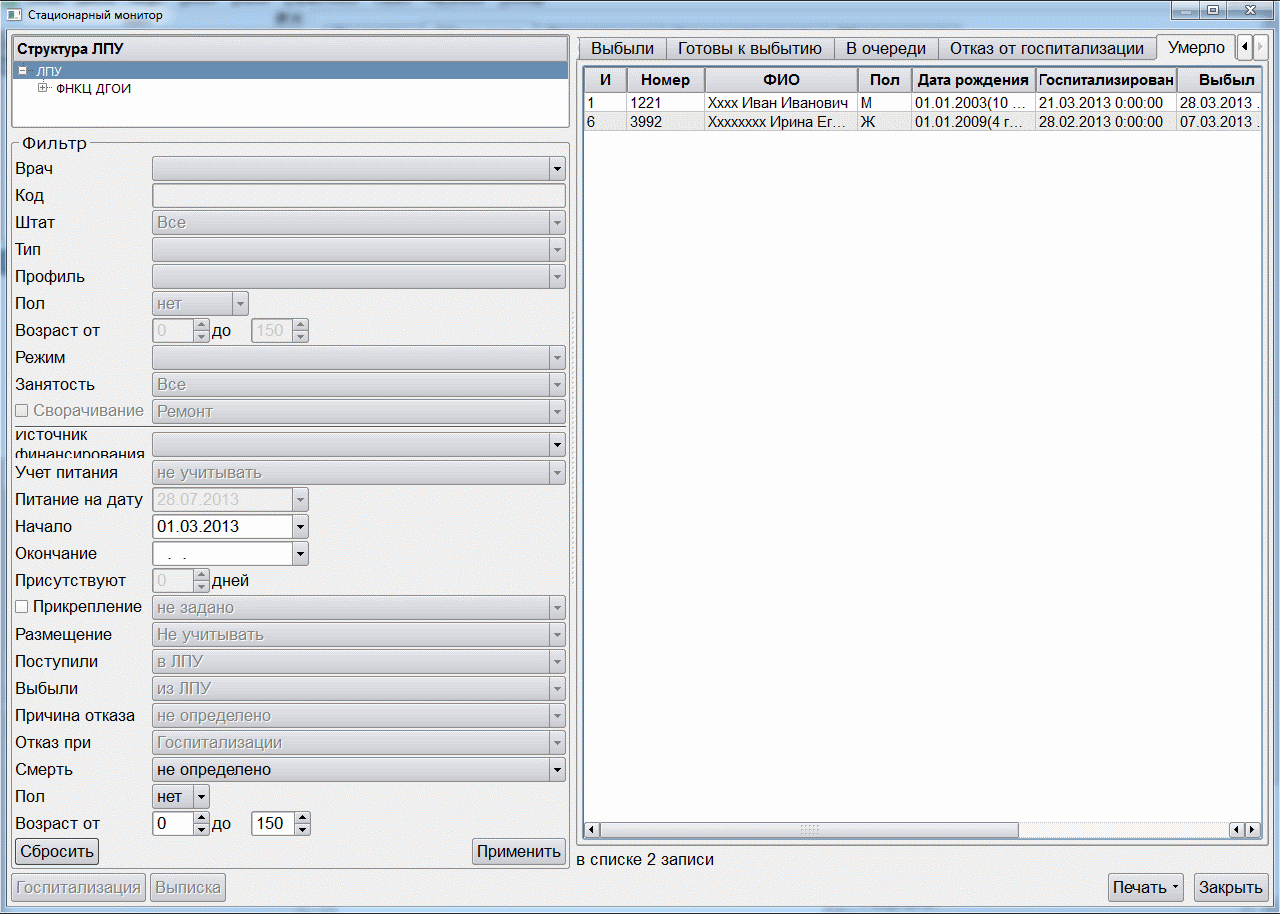
\includegraphics[width = 1\textwidth ,keepaspectratio]{st_mon_umer}
   \caption{Стационарный монитор. Вкладка <<Умерло>>}
   \label{img_st_mon_umer}
\end{figure}

Если в дереве структуры ЛПУ выбрано какое-либо подразделение, то список умерших будет показан только по этому подразделению. По умолчанию показывается список умерших по всему ЛПУ.

На данной вкладке возможна фильтрация по следующим параметрам:
\begin{itemize}
 \item \dm{Врач} – поиск по фамилии врача, который являлся лечащим врачом на момент закрытия обращения.
 \item \dm{Начало} – дата начала периода для отбора.
 \item \dm{Окончание} – дата окончания периода отбора.
 \item При выборе флажка \dm{Прикрепление} следует указать тип прикрепления, выбрав его из списка справа.
 \item \dm{Смерть} – причина смерти выбирается из списка.
 \item \dm{Пол} – выбирается из списка.
 \item \dm{Возраст} – можно выбрать пациентов определенной возрастной группы, указав границы возрастной группы в годах.
\end{itemize}
 
После того, как параметры фильтрации заданы, следует нажать кнопку \btn{Применить}, в области данных будет отображен список отказных пациентов, отобранных согласно указанным условиям. При нажатии на кнопку \btn{Сбросить}, параметры фильтрации возвращаются к настройкам по умолчанию.

Для вывода на печать списка умерших пациентов нужно нажать кнопку \btn{Печать} в правом нижнем углу окна и в появившемся меню выбрать пункт \dm{Сводка}. Откроется окно предварительного просмотра печати. Для отправки документа на принтер, необходимо нажать кнопку \btn{{Печатать}}  в окне предварительного просмотра печати, для сохранения списка в файл – кнопку \btn{Сохранить}.

Для открытия карточки обращения пациента следует дважды щелкнуть по соответствующей строке в списке левой кнопкой мыши либо щелкнуть правой кнопкой мыши и в появившемся контекстном меню выбрать пункт \dm{Открыть обращение}.

\subsection{Формирование статистических отчетов по работе стационара}

В \tmis~реализованы следующие статистические отчеты по работе стационара:
\begin{itemize}
 \item Сведения о деятельности стационара (Форма №14);
 \item Сведения о деятельности  дневных  стационаров  лечебно-профилакти\-чес\-ких учреждений (Форма №14ДС).
\end{itemize}

Вызов отчетов выполняется в пункте \mm{Анализ \str Стационар} главного меню. Далее следует выбрать название статистического отчета, а затем название раздела. Формирование отчетов производится отдельно по каждому разделу отдельно. После выбора раздела отчета откроется окно параметров отчета, где необходимо указать период формирования (как правило, отчет формируется за весь предыдущий год) и подразделение (Рисунок \ref{img_st_strep_par}). По умолчанию отчет формируется по всему ЛПУ.

\begin{figure}[ht]\centering
   \includegraphics[width = 0.5\textwidth ,keepaspectratio]{st_strep_par}
   \caption{Параметры формирования отчетов}
   \label{img_st_strep_par}
\end{figure}

После нажатия кнопки \btn{OK}  будет открыто окно предварительного просмотра выбранного раздела отчета (Рисунок \ref{img_st_strep_prn}). Для отправки отчета на принтер следует нажать кнопку \btn{Печатать}. Для сохранения отчета в файл необходимо нажать кнопку \btn{Сохранить}, выбрать папку для сохранения и формат файла, ввести название файла, а затем снова нажать кнопку \btn{Сохранить}. Нажатие кнопки \btn{Повторить} позволяет вернуться к окну ввода параметров отчета (Рисунок \ref{img_st_strep_par}) и сформировать отчет заново с новыми параметрами.

\begin{figure}[h!]\centering
   \includegraphics[width = 0.8\textwidth ,keepaspectratio]{st_strep_prn}
   \caption{Предварительный просмотр раздела (2000) отчета}
   \label{img_st_strep_prn}
\end{figure}

Необходимо последовательно сформировать все разделы отчета за один и тот же период, вывести их на печать или сохранить в отдельные файлы.

\begin{vnim} 
Формирование отчета за длительный период может занять продолжительное время.
\end{vnim}